\chapterimage{chap2.jpg}
\chapter{线性表}

\section{线性表的定义和基本操作}
\begin{definition}[线性表]
    $$L=(a_{1},a_{2},a_{3},\dots,a_{i},a_{i+1},\dots,a_{n})$$
    \begin{enumerate}
        \item 有相同数据类型的 $n$ 个数据元素的有限序列
        \item 存在唯一的一个被称作“第一个”的数据元素
        \item 存在唯一的一个被称作“最后一个”的数据元素
        \item 除第一个外,每个数据元素有且仅有一个直接前驱
        \item 除最后一个外,每个数据元素有且仅有一个直接后继
    \end{enumerate}
\end{definition}

\begin{definition}[线性表基本操作]
    \begin{enumerate}
        \item $\mathbf{InitList(\& L)}$  初始化线性表,构造一个空的线性表 $L$
        \item $\mathbf{DestroyList(\& L)}$  销毁线性表,销毁线性表 $L$
        \item $\mathbf{ListInsert(\&L,i,e)}$ 插入操作,在线性表 $L$ 的第 $i$ 个位置插入元素 $e$
        \item $\mathbf{ListDelete(\&L,i,\&e)}$ 删除操作,删除线性表 $L$ 的第 $i$ 个位置的元素,并用 $e$ 返回其值
        \item $\mathbf{GetElem(L,i,\&e)}$ 取值操作,返回线性表 $L$ 的第 $i$ 个位置的元素
        \item $\mathbf{LocateElem(L,e)}$ 定位操作,在线性表 $L$ 中查找与给定值 $e$ 相等的元素
        \item $\mathbf{Length(L)}$ 求表长,返回线性表 $L$ 的元素个数
        \item $\mathbf{Empty(L)}$ 判空操作,若 $L$ 为空表,则返回 $\text{TRUE}$,否则返回 $\text{FALSE}$
        \item $\mathbf{PrintList(L)}$ 输出操作,按顺序输出线性表 $L$ 的所有元素 
    \end{enumerate}
\end{definition}

\section{线性表的顺序表示}
\subsection{顺序表}
\begin{definition}[顺序表]
    \begin{enumerate}
        \item 用顺序存储的方式实现线性表
        \item 顺序存储: 把逻辑上相邻的元素存储在物理上相邻的存储单元中,元素之间的关系由存储单元之间的邻接关系来体现
    \end{enumerate}
\end{definition}

\begin{figure}[H]
    \centering
    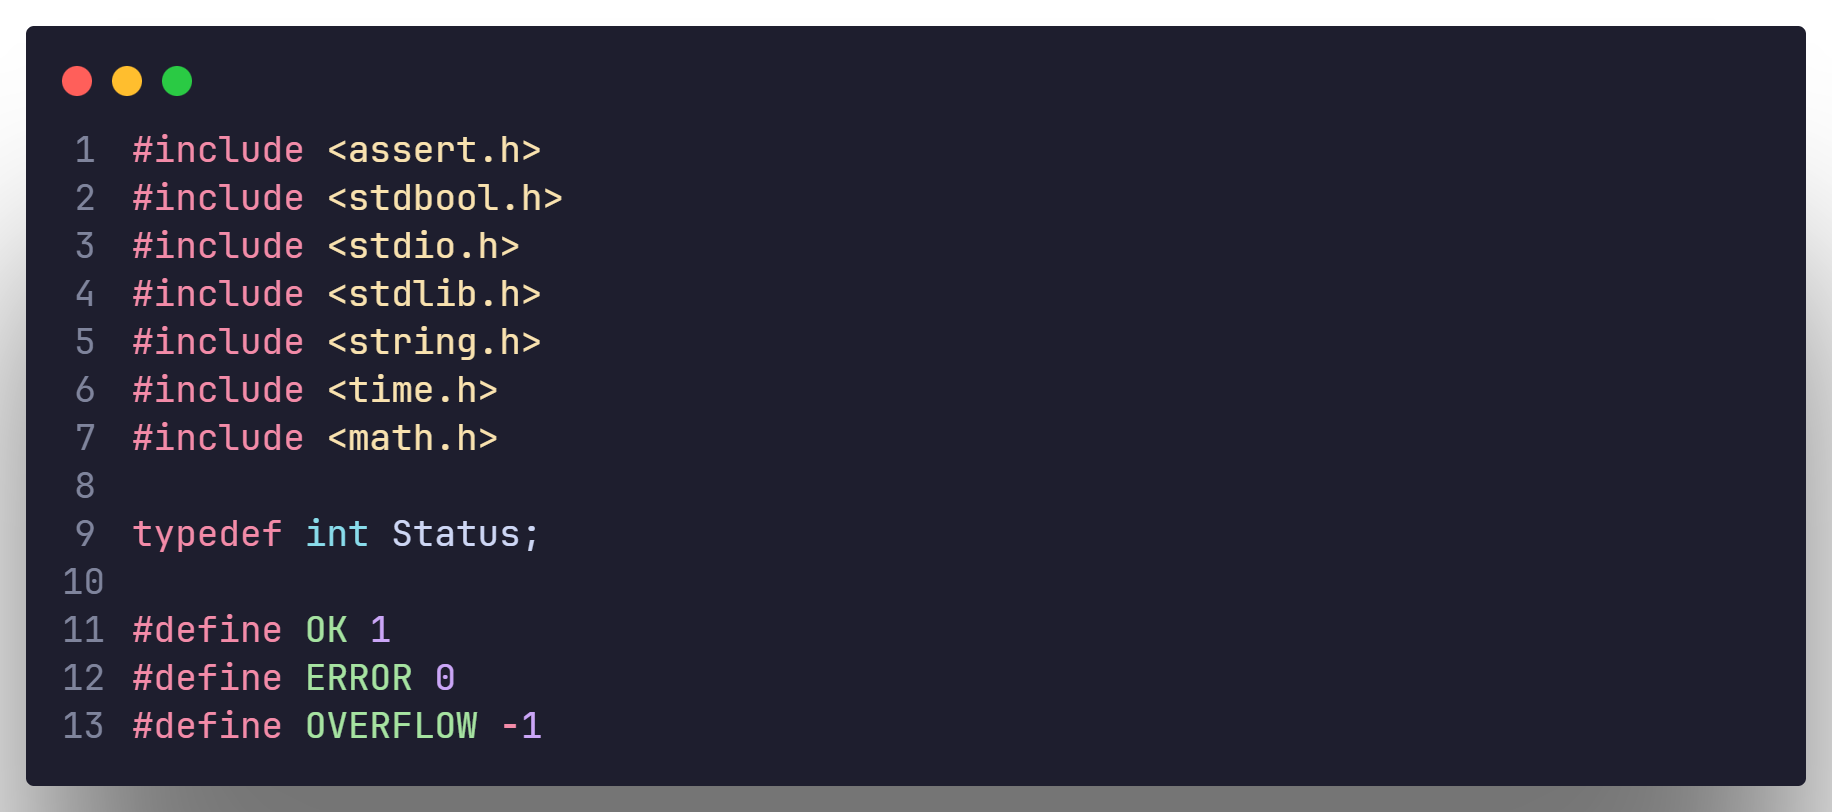
\includegraphics[scale=0.2]{"figure/Note/LinearList/common.png"}
\end{figure} 

\subsubsection{顺序表定义和函数声明}
\begin{figure}[H]
    \centering
    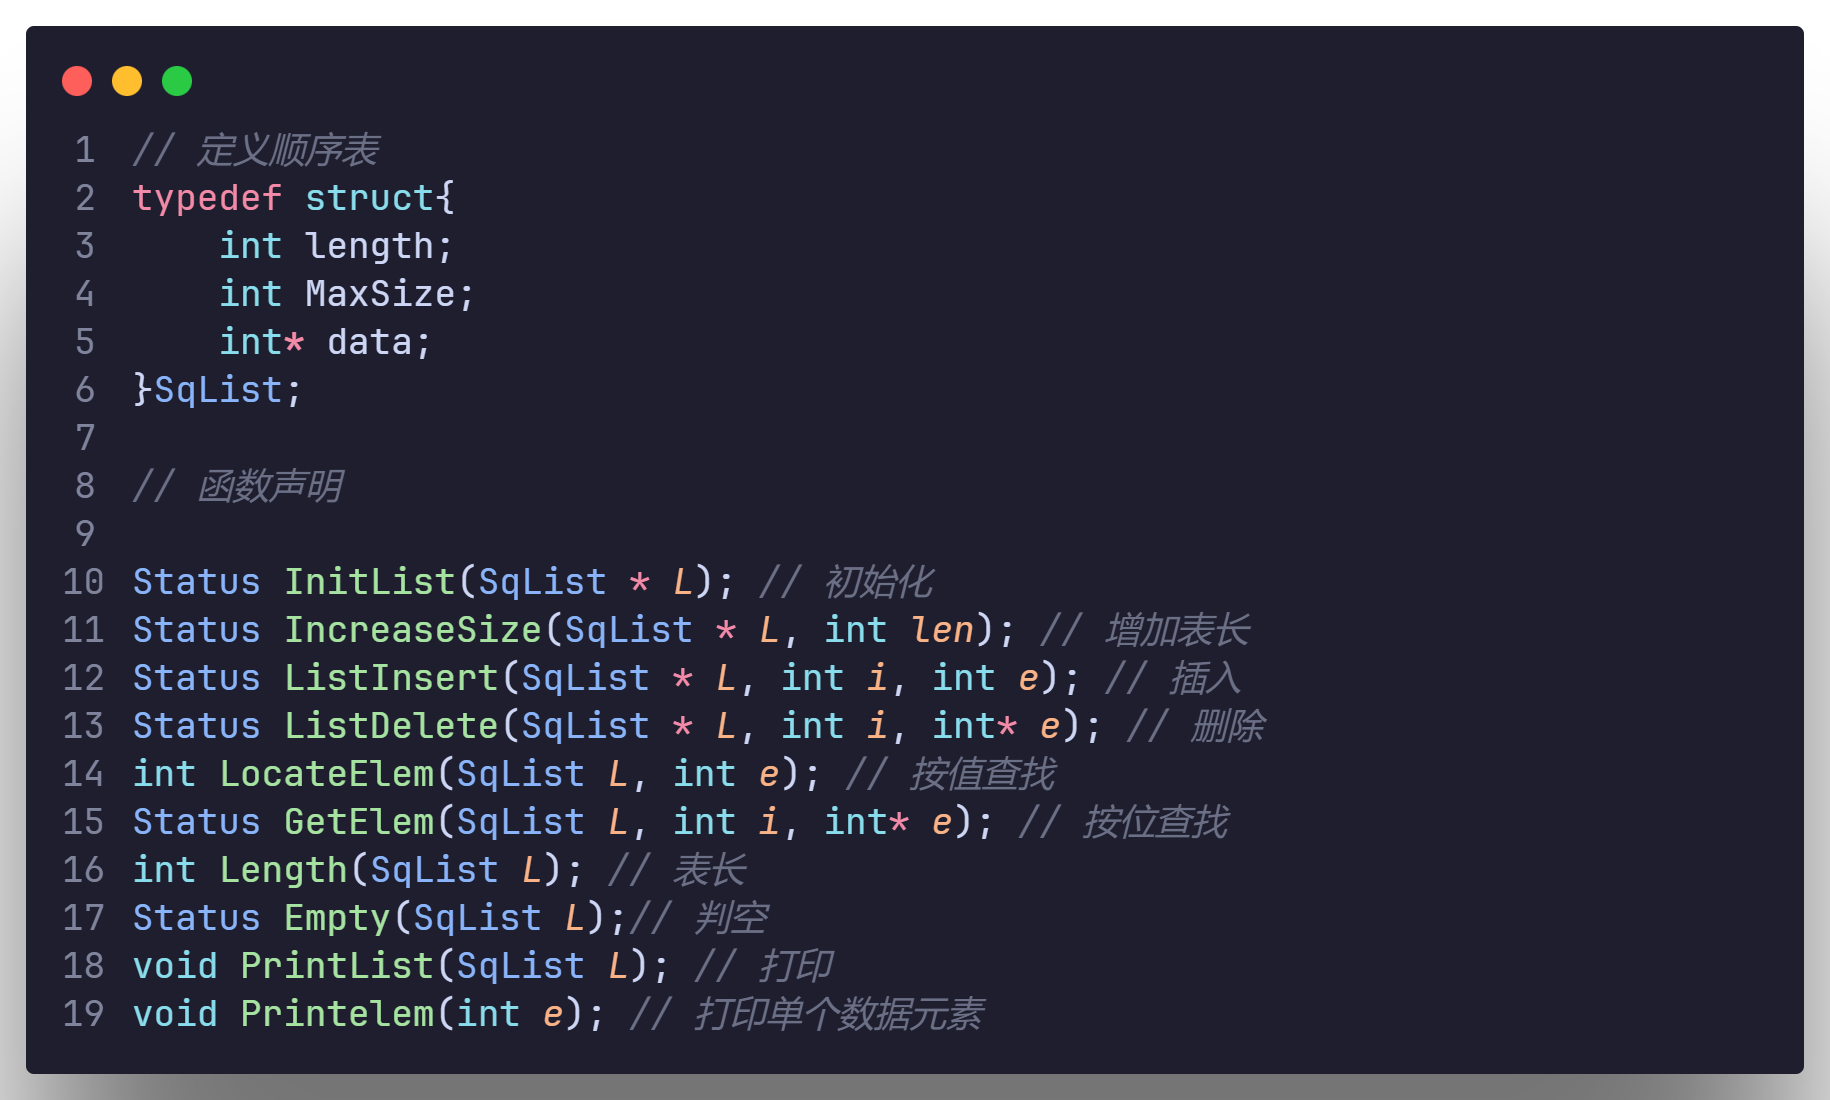
\includegraphics[scale=0.2]{"figure/Note/LinearList/SqFunction.png"}
\end{figure} 

\subsubsection{顺序表初始化}

\begin{figure}[H]
    \centering
    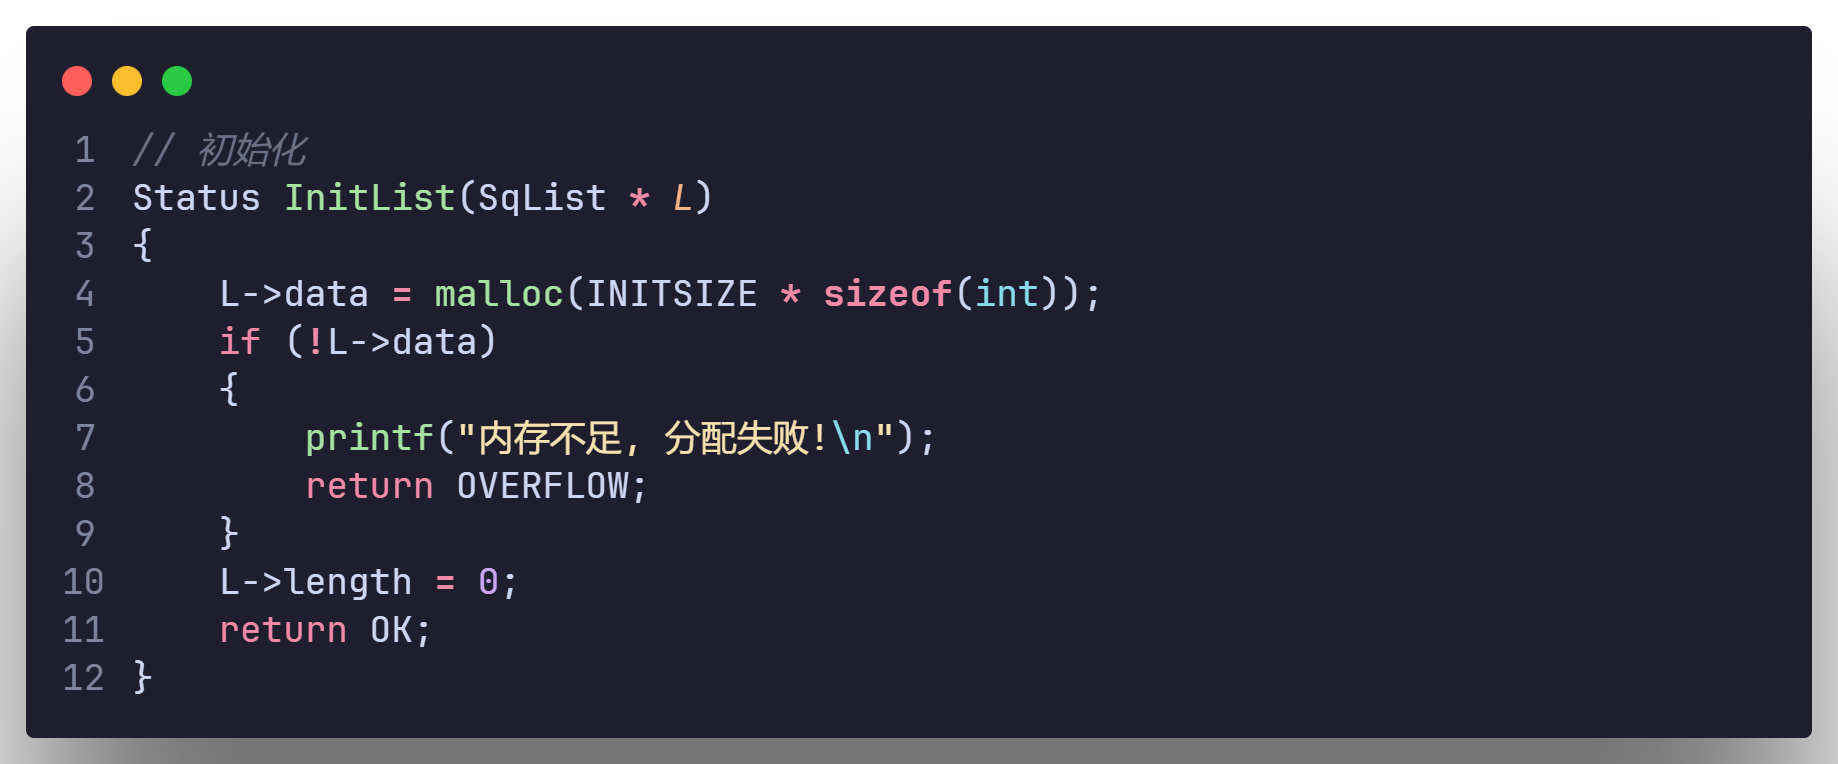
\includegraphics[scale=0.2]{"figure/Note/LinearList/SqInit.png"}
\end{figure} 

\subsubsection{顺序表增加}

\begin{figure}[H]
    \centering
    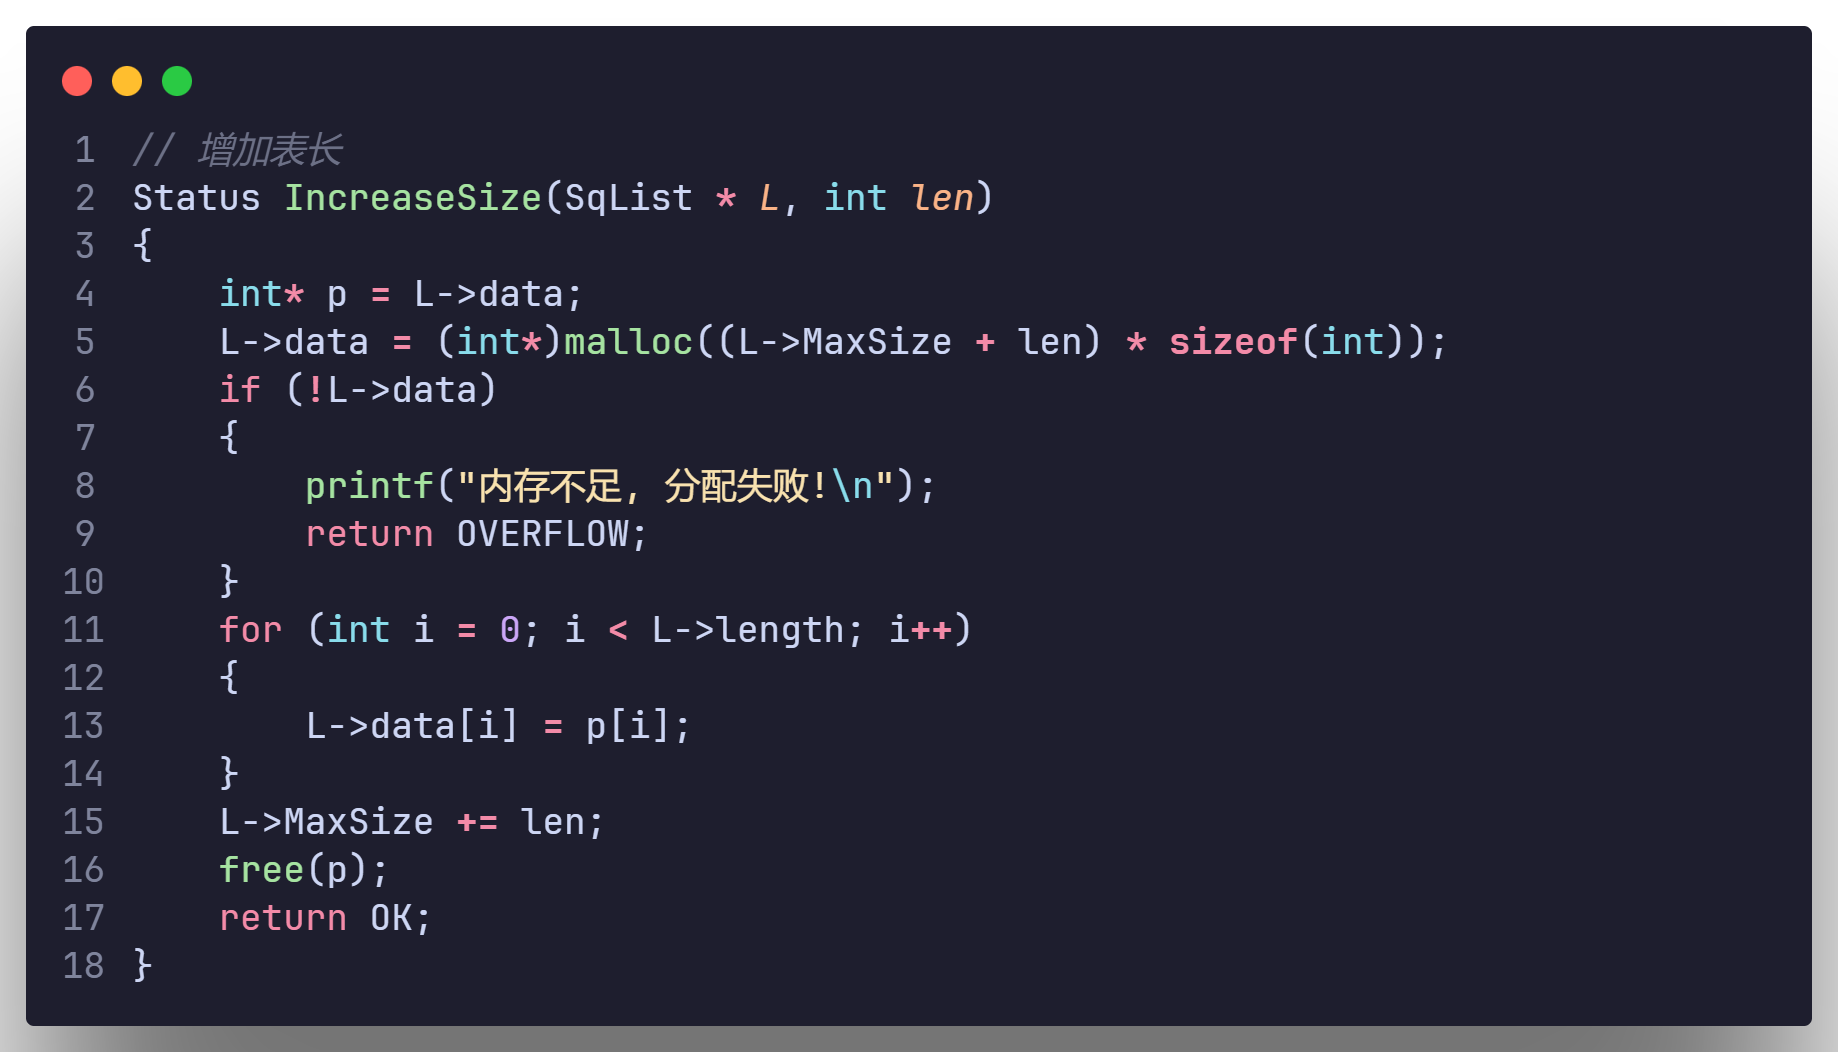
\includegraphics[scale=0.2]{"figure/Note/LinearList/SqIncrease.png"}
\end{figure} 

\subsubsection{顺序表插入}

\begin{figure}[H]
    \centering
    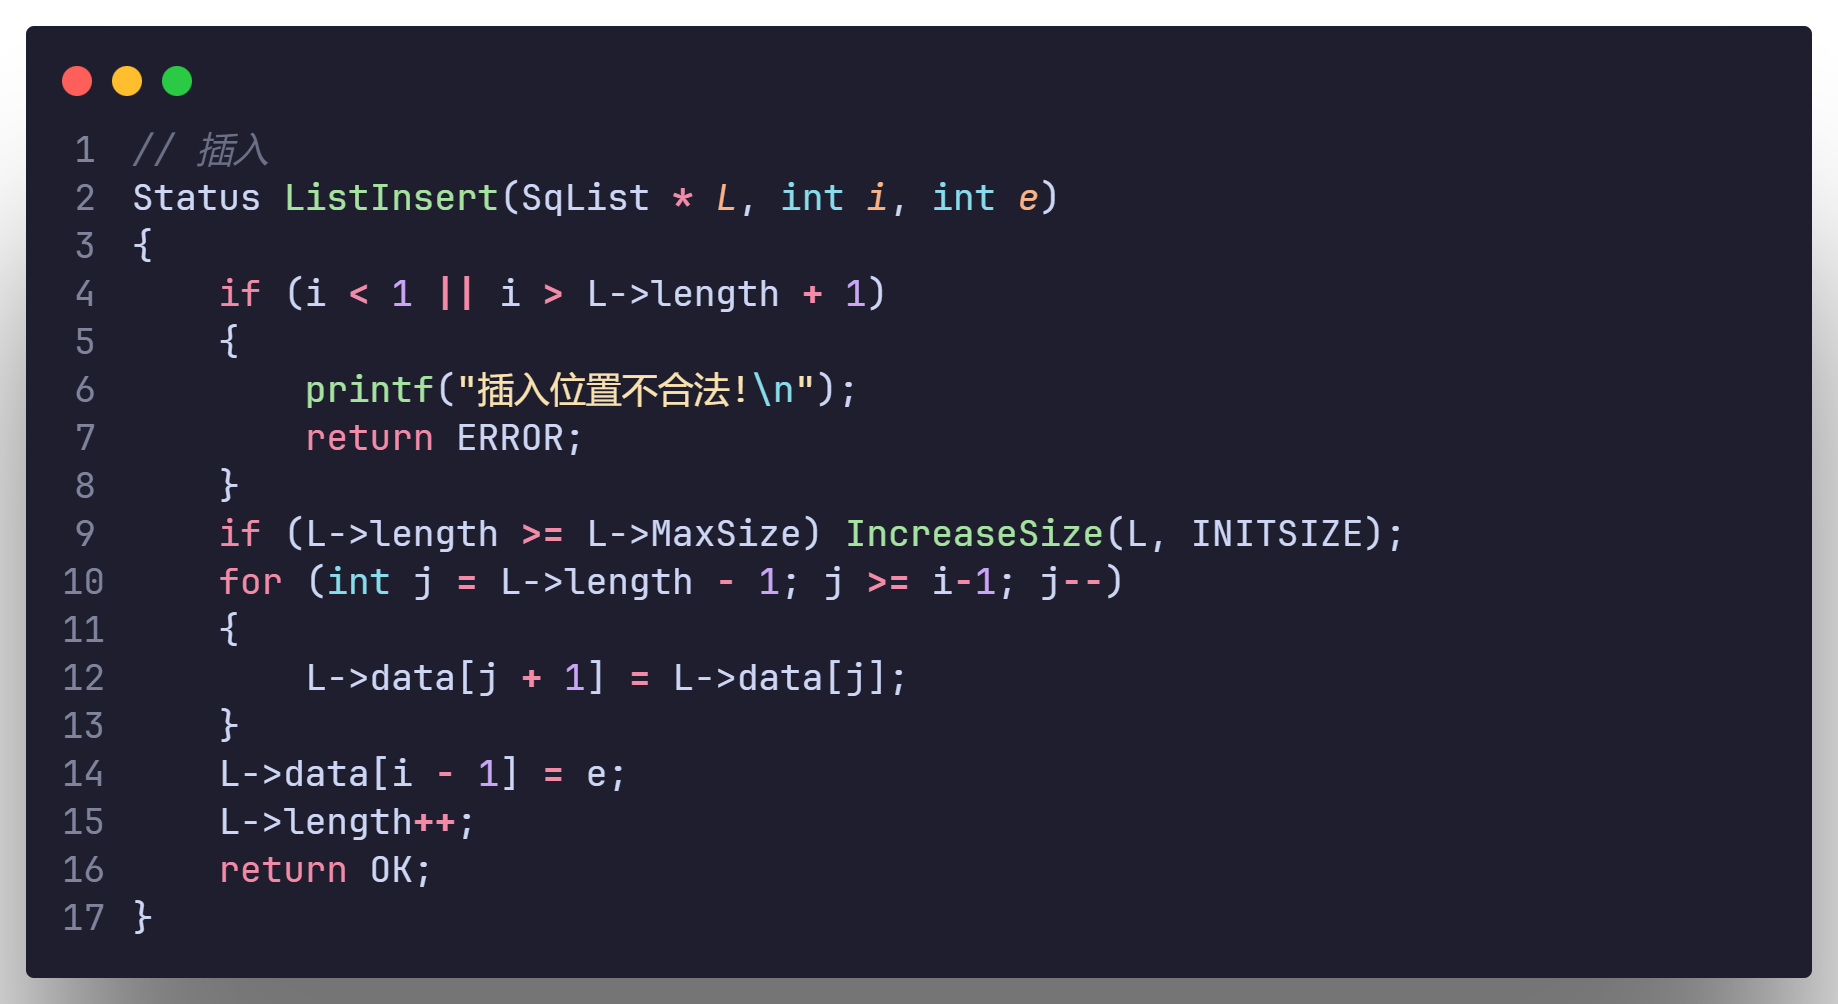
\includegraphics[scale=0.2]{"figure/Note/LinearList/SqInsert.png"}
\end{figure} 

\subsubsection{顺序表删除}

\begin{figure}[H]
    \centering
    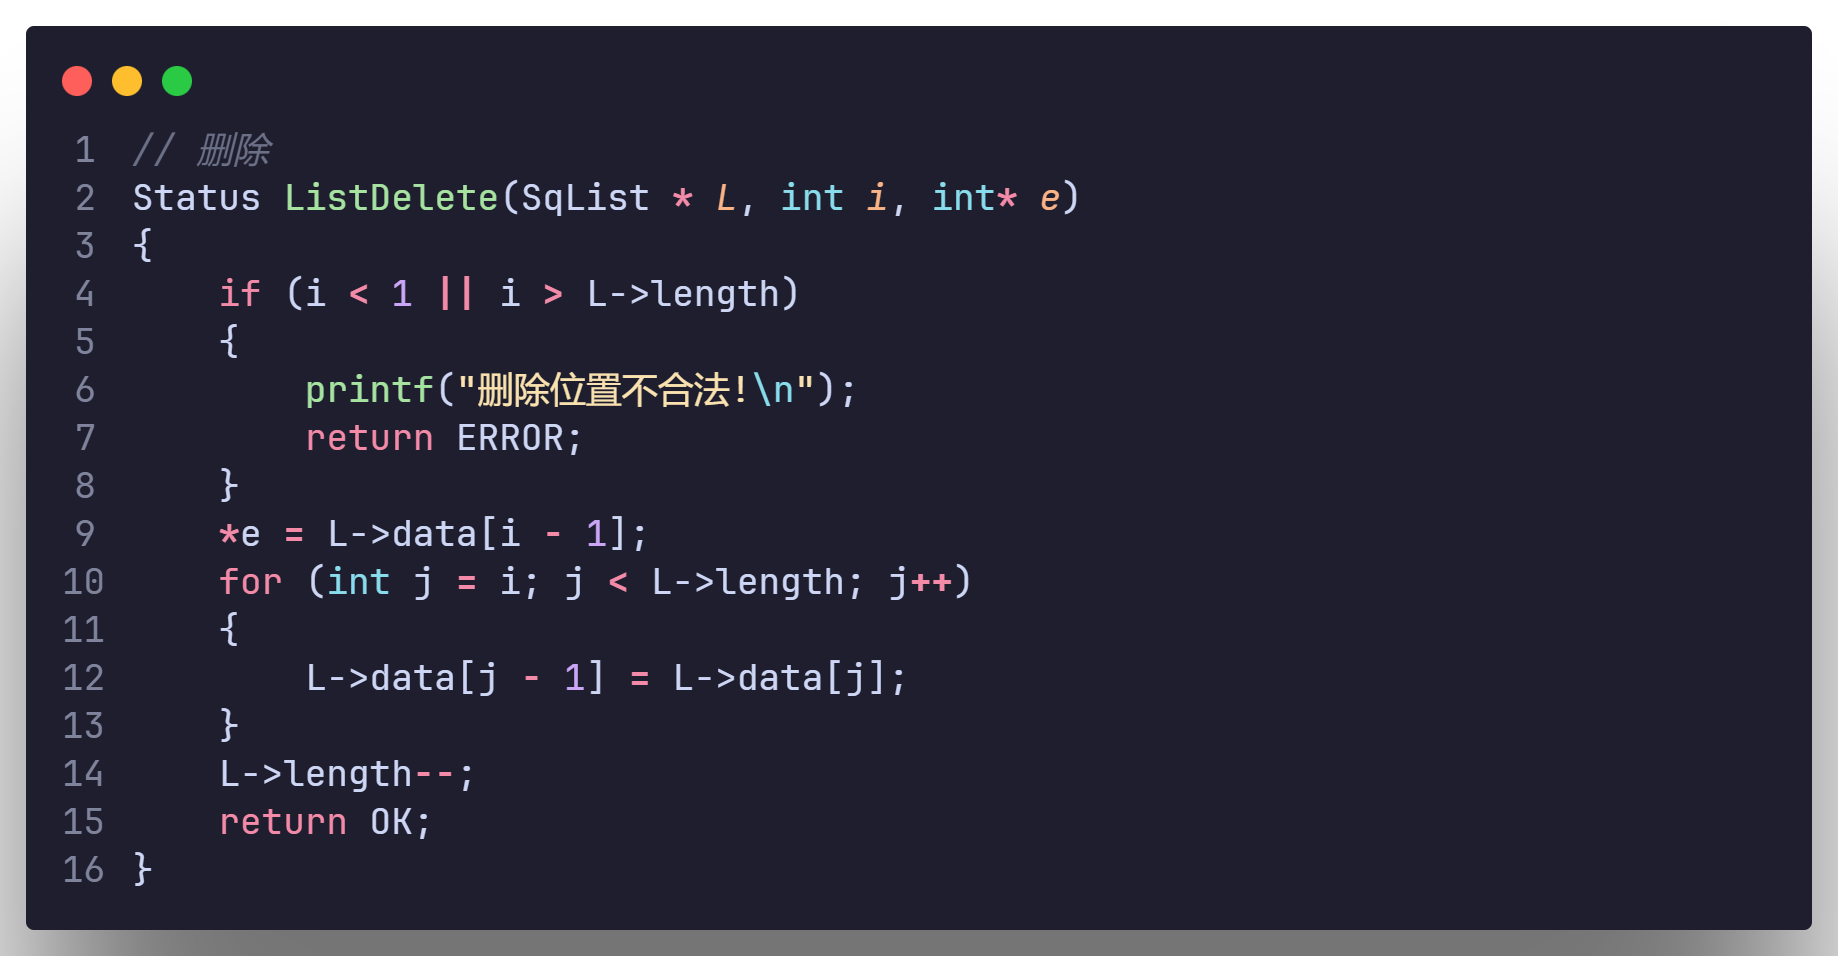
\includegraphics[scale=0.2]{"figure/Note/LinearList/SqDel.png"}
\end{figure} 

\subsubsection{顺序表查找}

(1). 按位置查找

\begin{figure}[H]
    \centering
    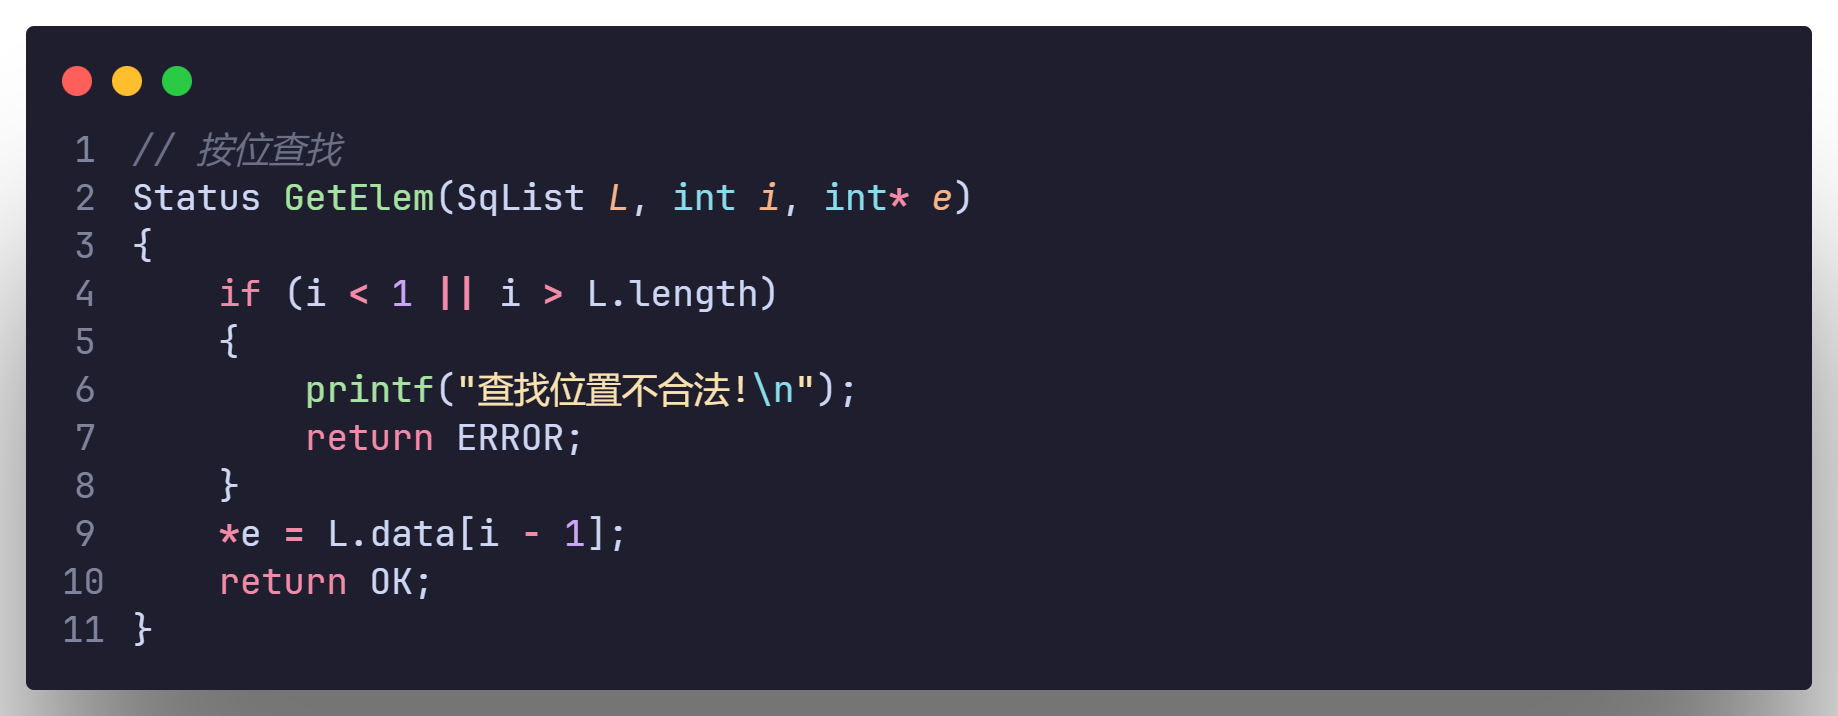
\includegraphics[scale=0.2]{"figure/Note/LinearList/SqNumSer.png"}
\end{figure} 

(2). 按值查找

\begin{figure}[H]
    \centering
    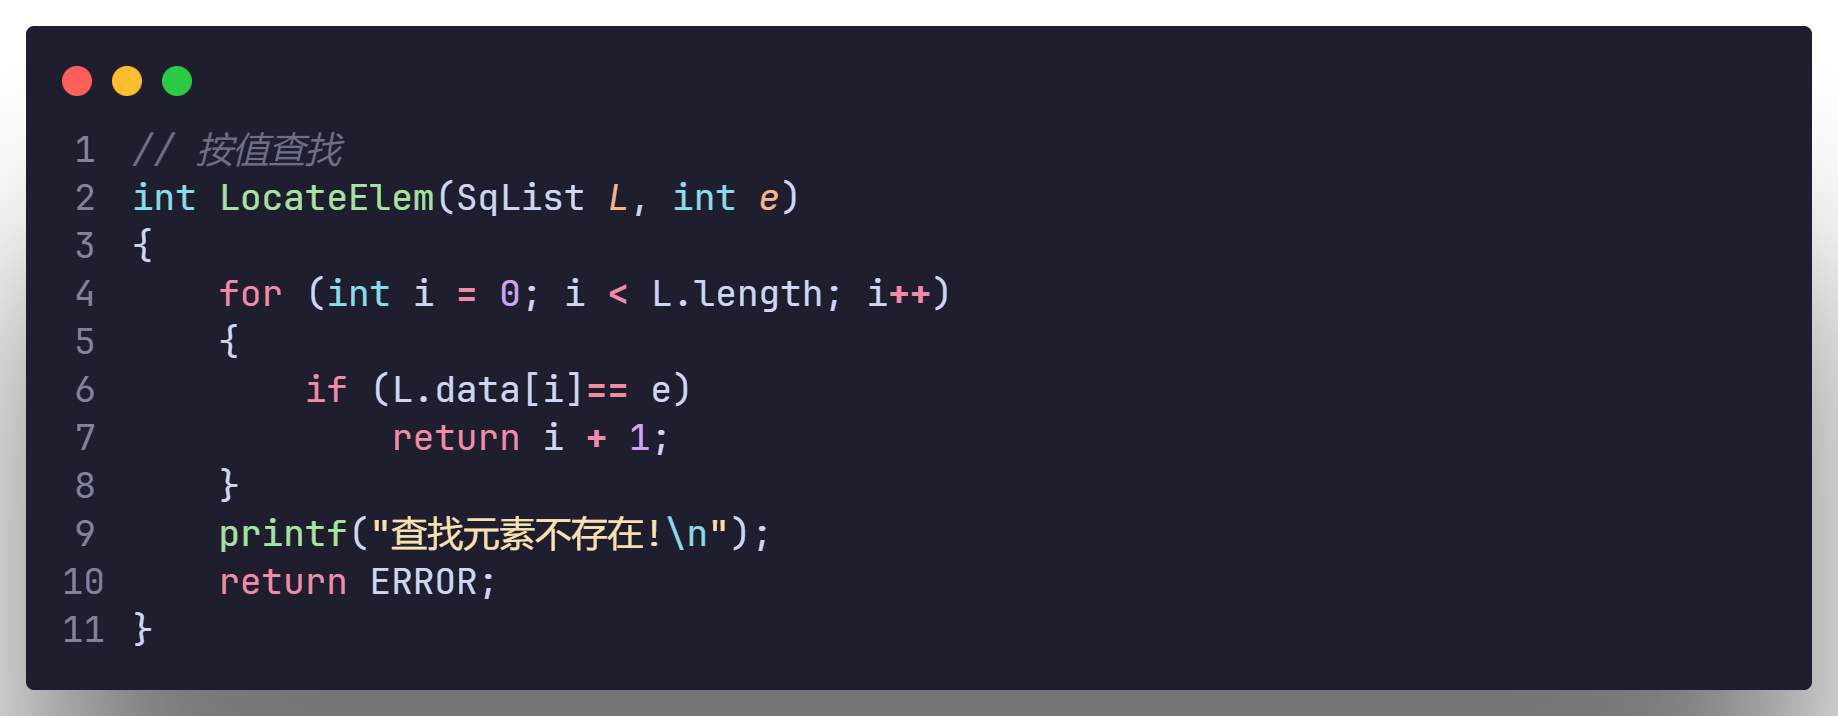
\includegraphics[scale=0.2]{"figure/Note/LinearList/SqItemSer.png"}
\end{figure} 


\subsubsection{顺序表辅助函数}

(1). $Length$ 

\begin{figure}[H]
    \centering
    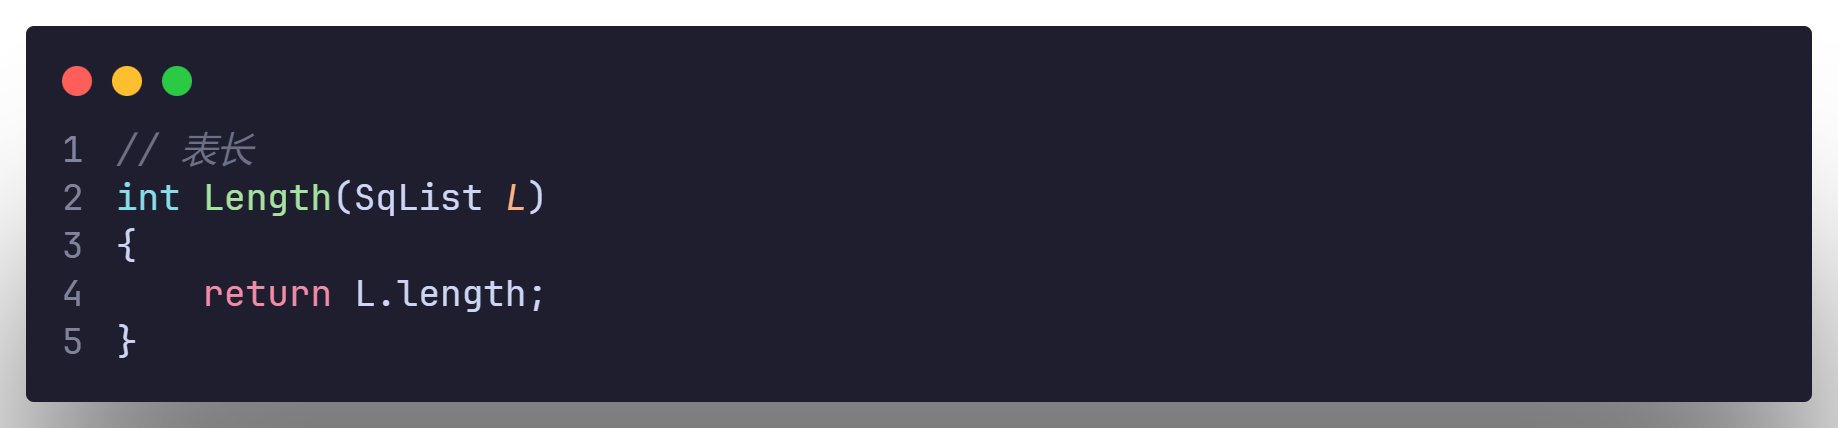
\includegraphics[scale=0.2]{"figure/Note/LinearList/SqLen.png"}
\end{figure} 

(2). $Empty$ 

\begin{figure}[H]
    \centering
    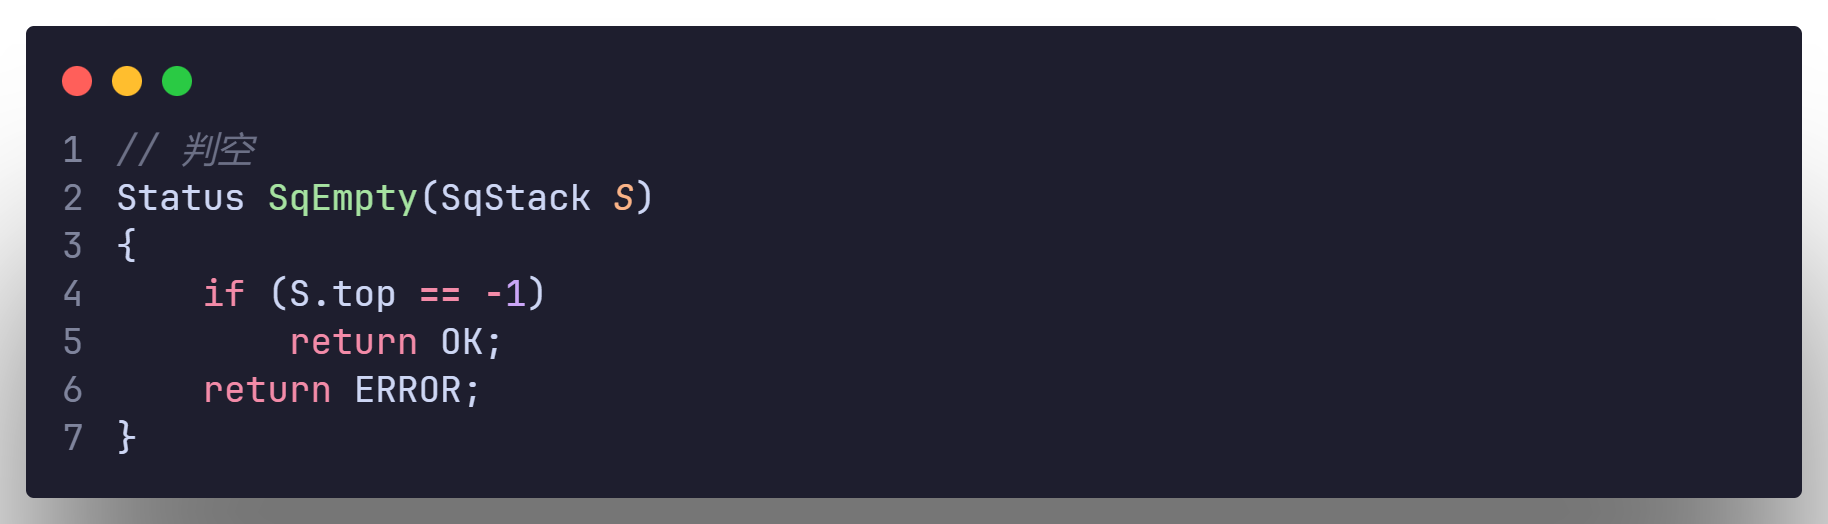
\includegraphics[scale=0.2]{"figure/Note/LinearList/SqEmpty.png"}
\end{figure} 

(3). $PrintList$

\begin{figure}[H]
    \centering
    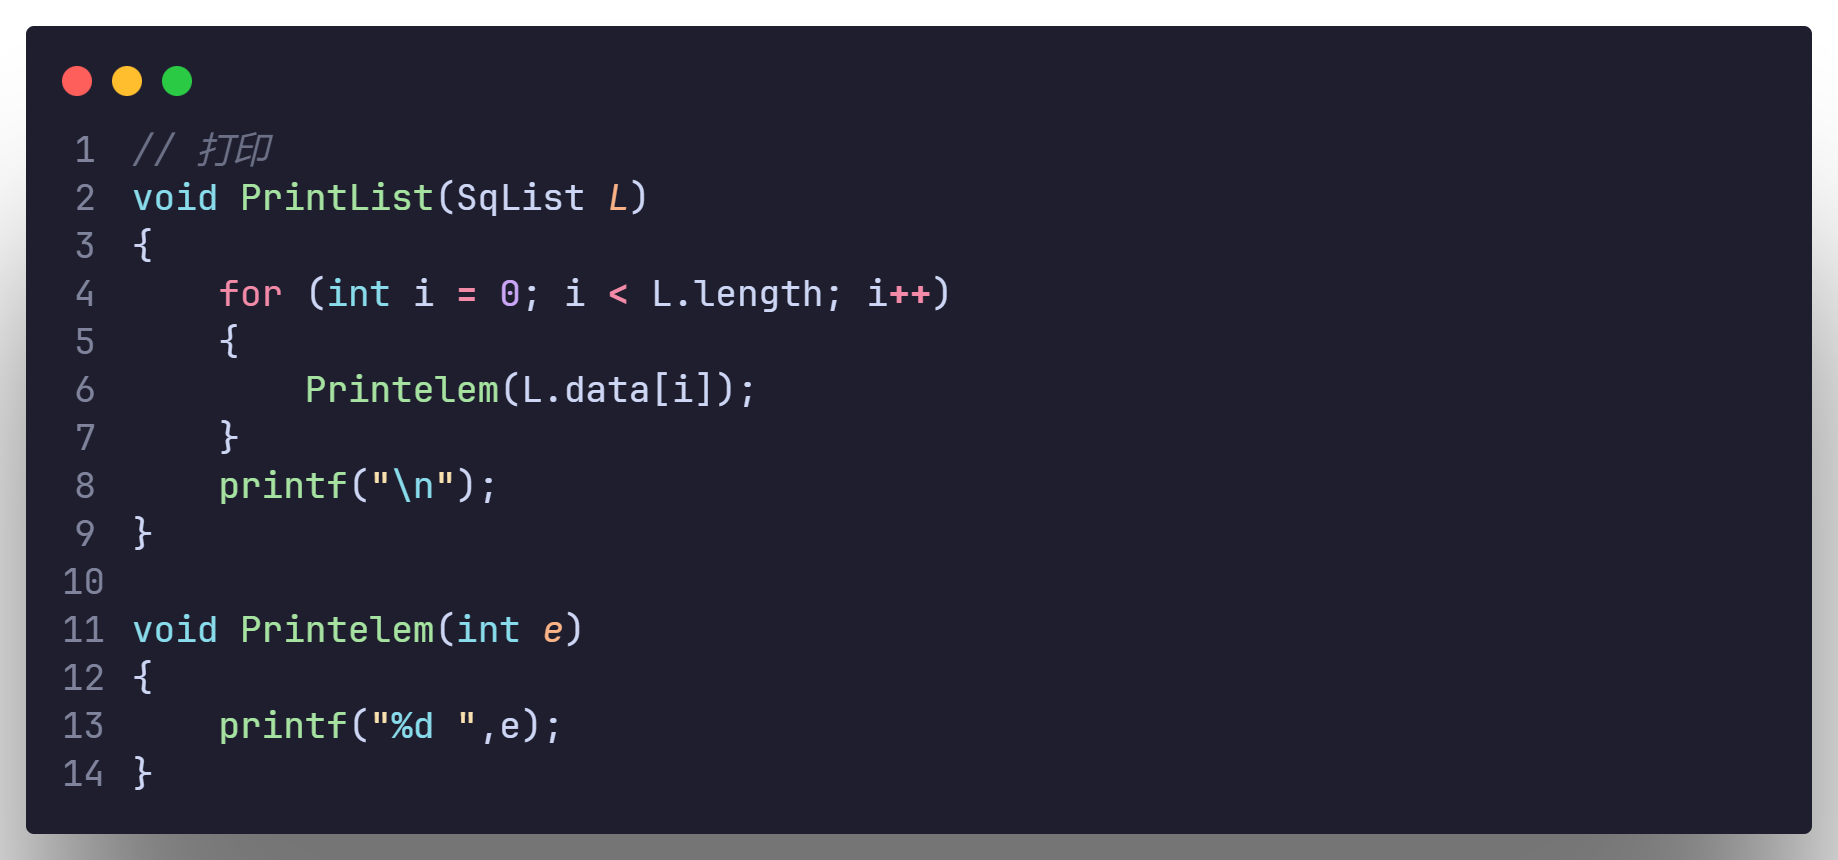
\includegraphics[scale=0.2]{"figure/Note/LinearList/SqPrint.png"}
\end{figure} 

\section{线性表的链式表示}
\subsection{单链表}
\begin{definition}[单链表]
    \begin{enumerate}
        \item 单链表第一个元素在删除和增加需要特殊处理
        \item 头插法和尾插法的区别, 头插法实现反置
        \item 在增删、初始化操作传入引用, 在判空、打印以及求表长传入值
    \end{enumerate}
\end{definition}
\subsubsection{单链表定义和函数声明}

\begin{figure}[H]
    \centering
    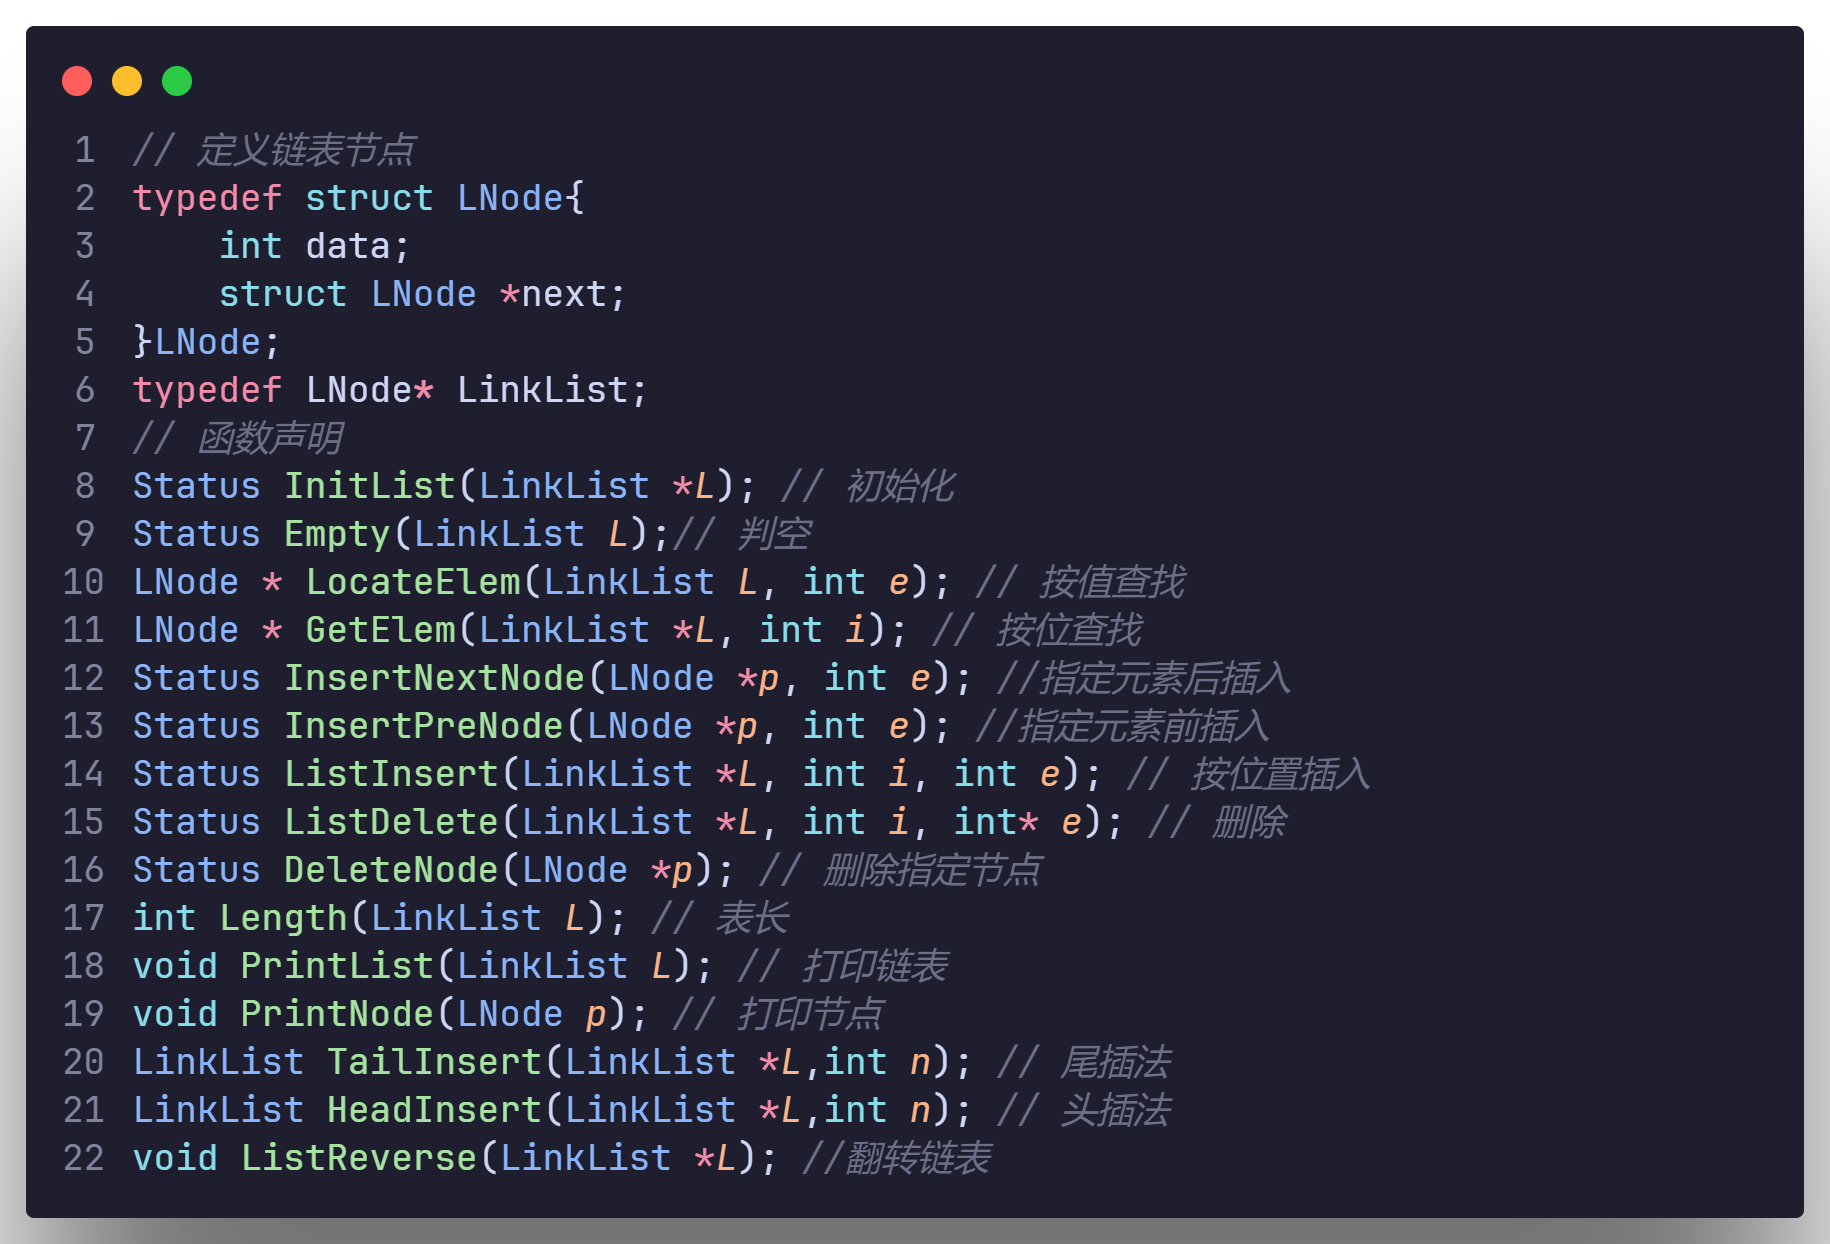
\includegraphics[scale=0.2]{"figure/Note/LinearList/SlFunction.png"}
\end{figure} 

\subsubsection{单链表初始化}

\begin{figure}[H]
    \centering
    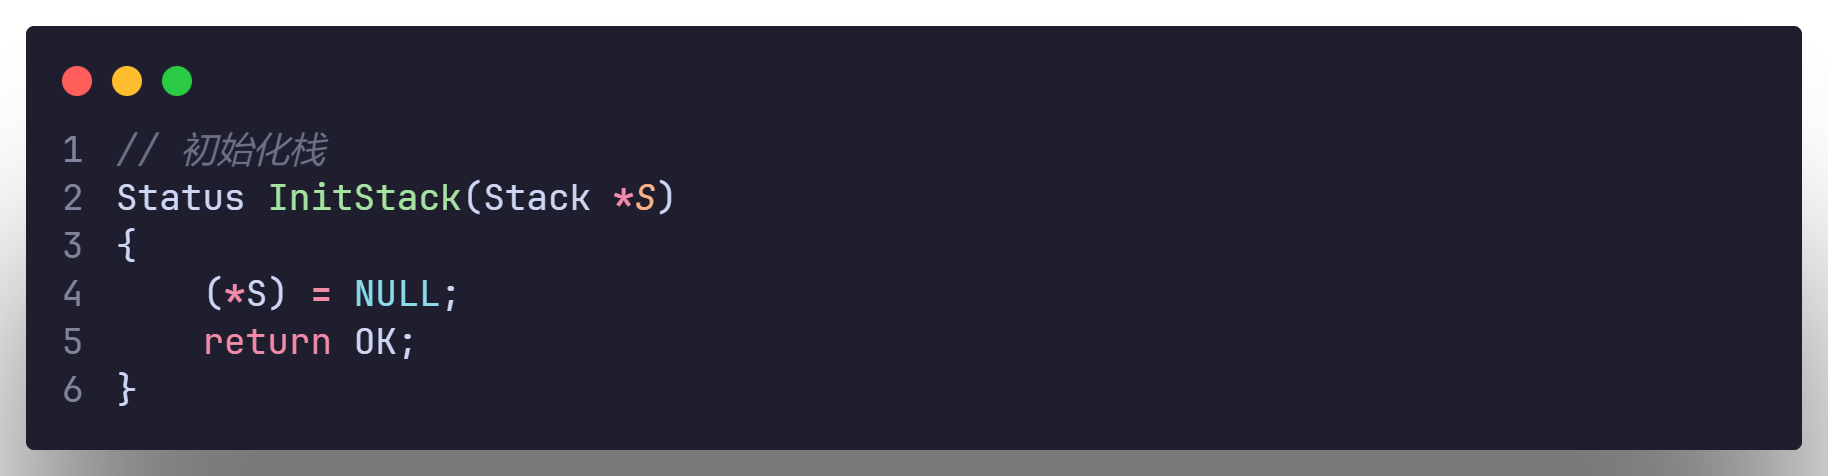
\includegraphics[scale=0.2]{"figure/Note/LinearList/SlInit.png"}
\end{figure} 

\subsubsection{单链表查找}

(1). 按位置查找
\begin{figure}[H]
    \centering
    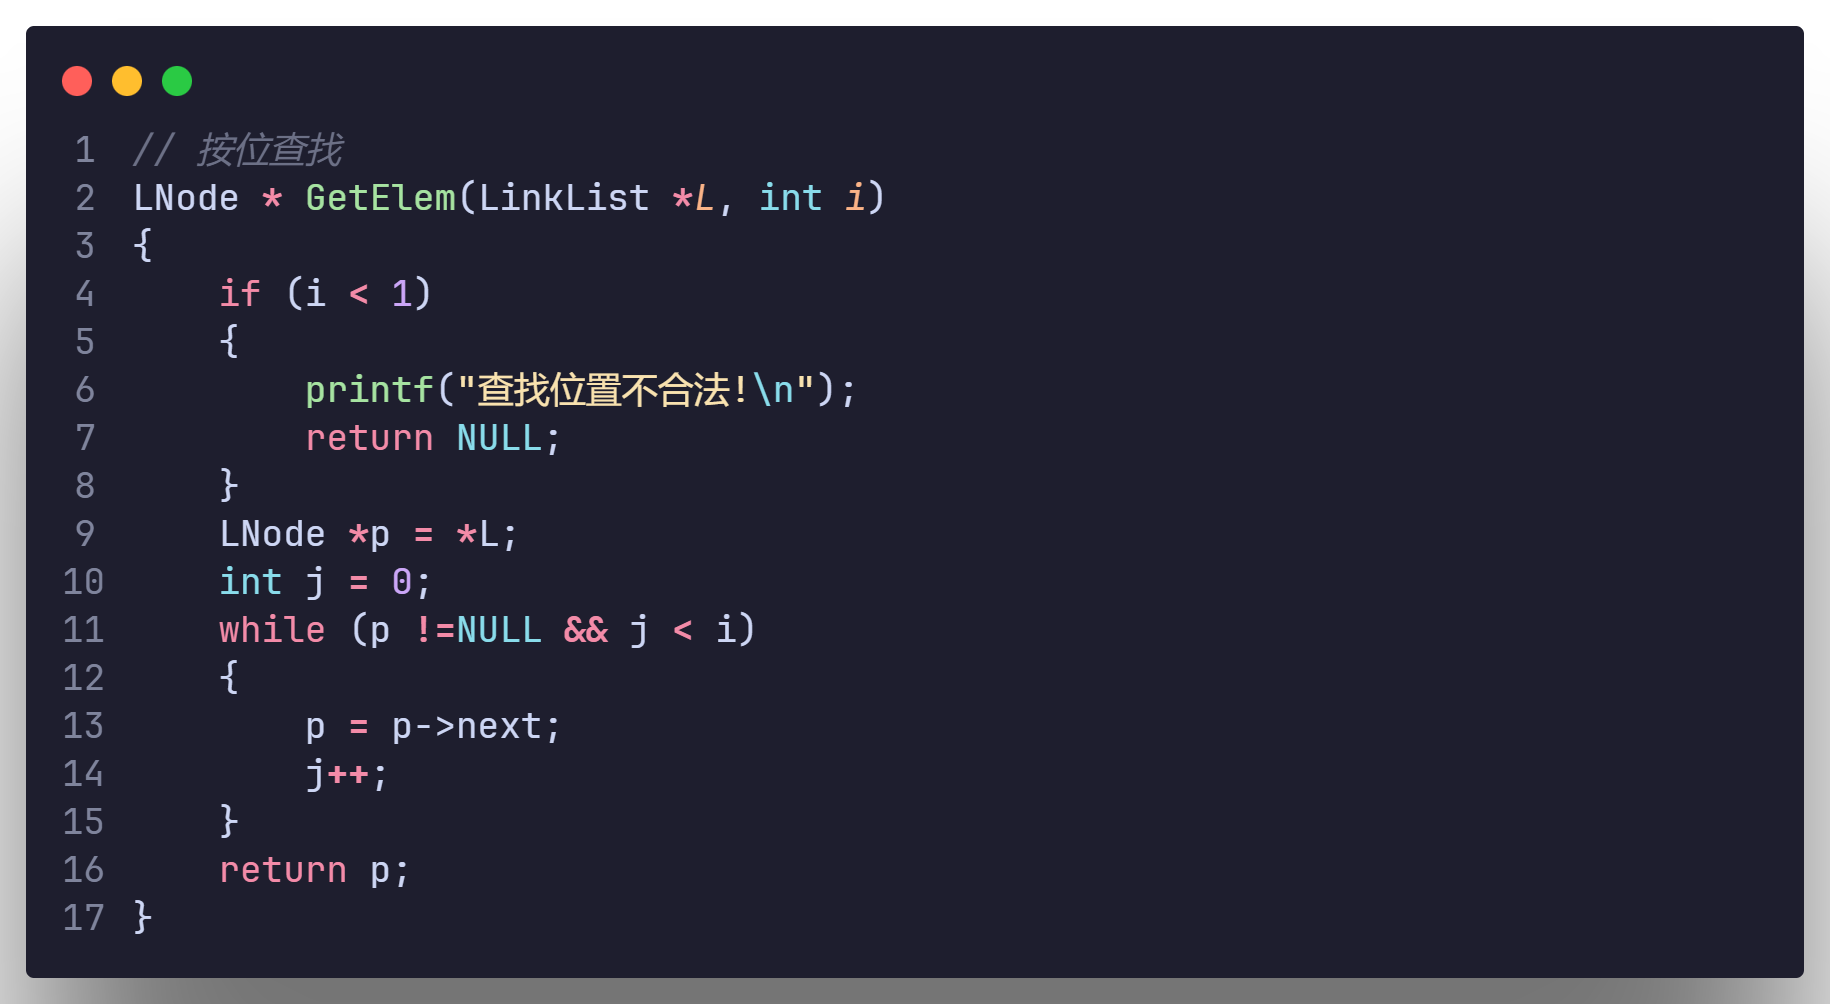
\includegraphics[scale=0.2]{"figure/Note/LinearList/SlNumSer.png"}
\end{figure} 

(2). 按值查找

\begin{figure}[H]
    \centering
    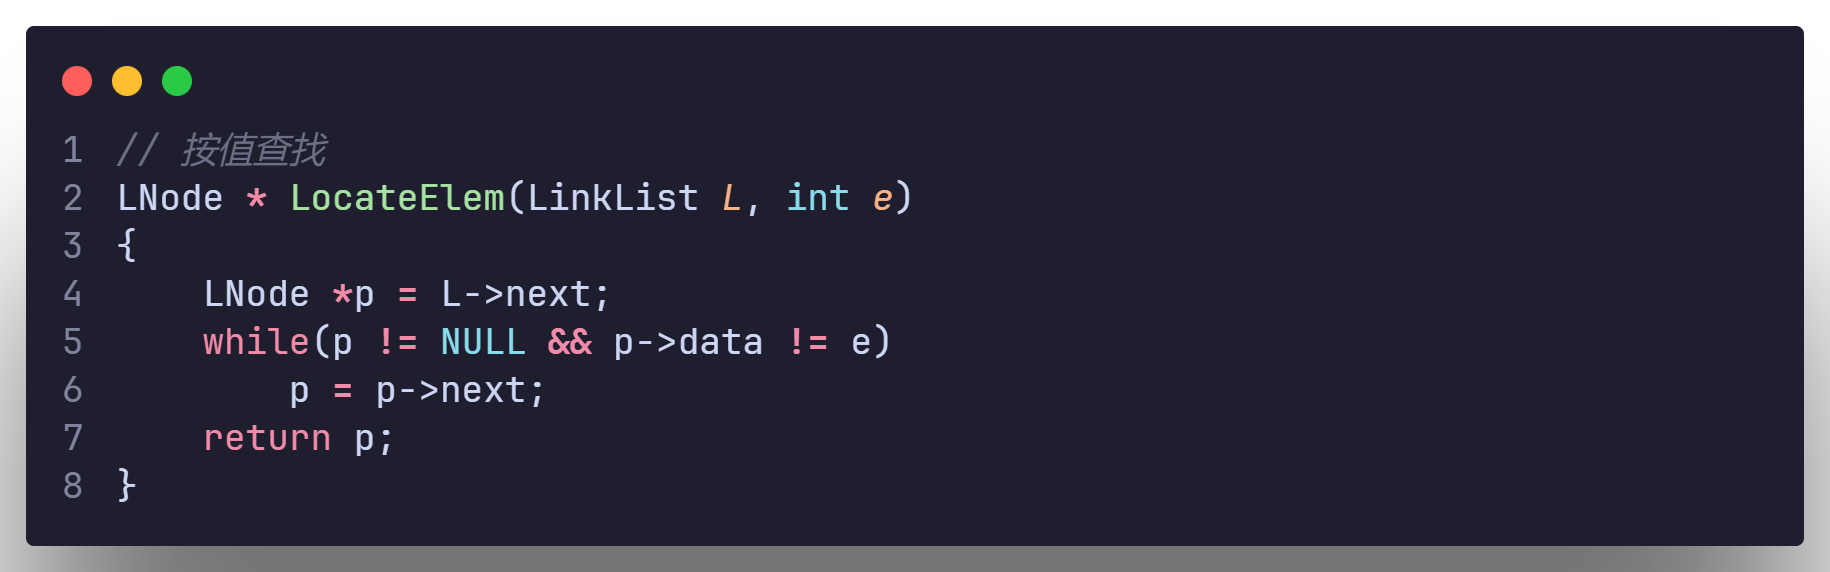
\includegraphics[scale=0.2]{"figure/Note/LinearList/SlItemSer.png"}
\end{figure} 

\subsubsection{单链表插入}

(1). 指定元素后插入

\begin{figure}[H]
    \centering
    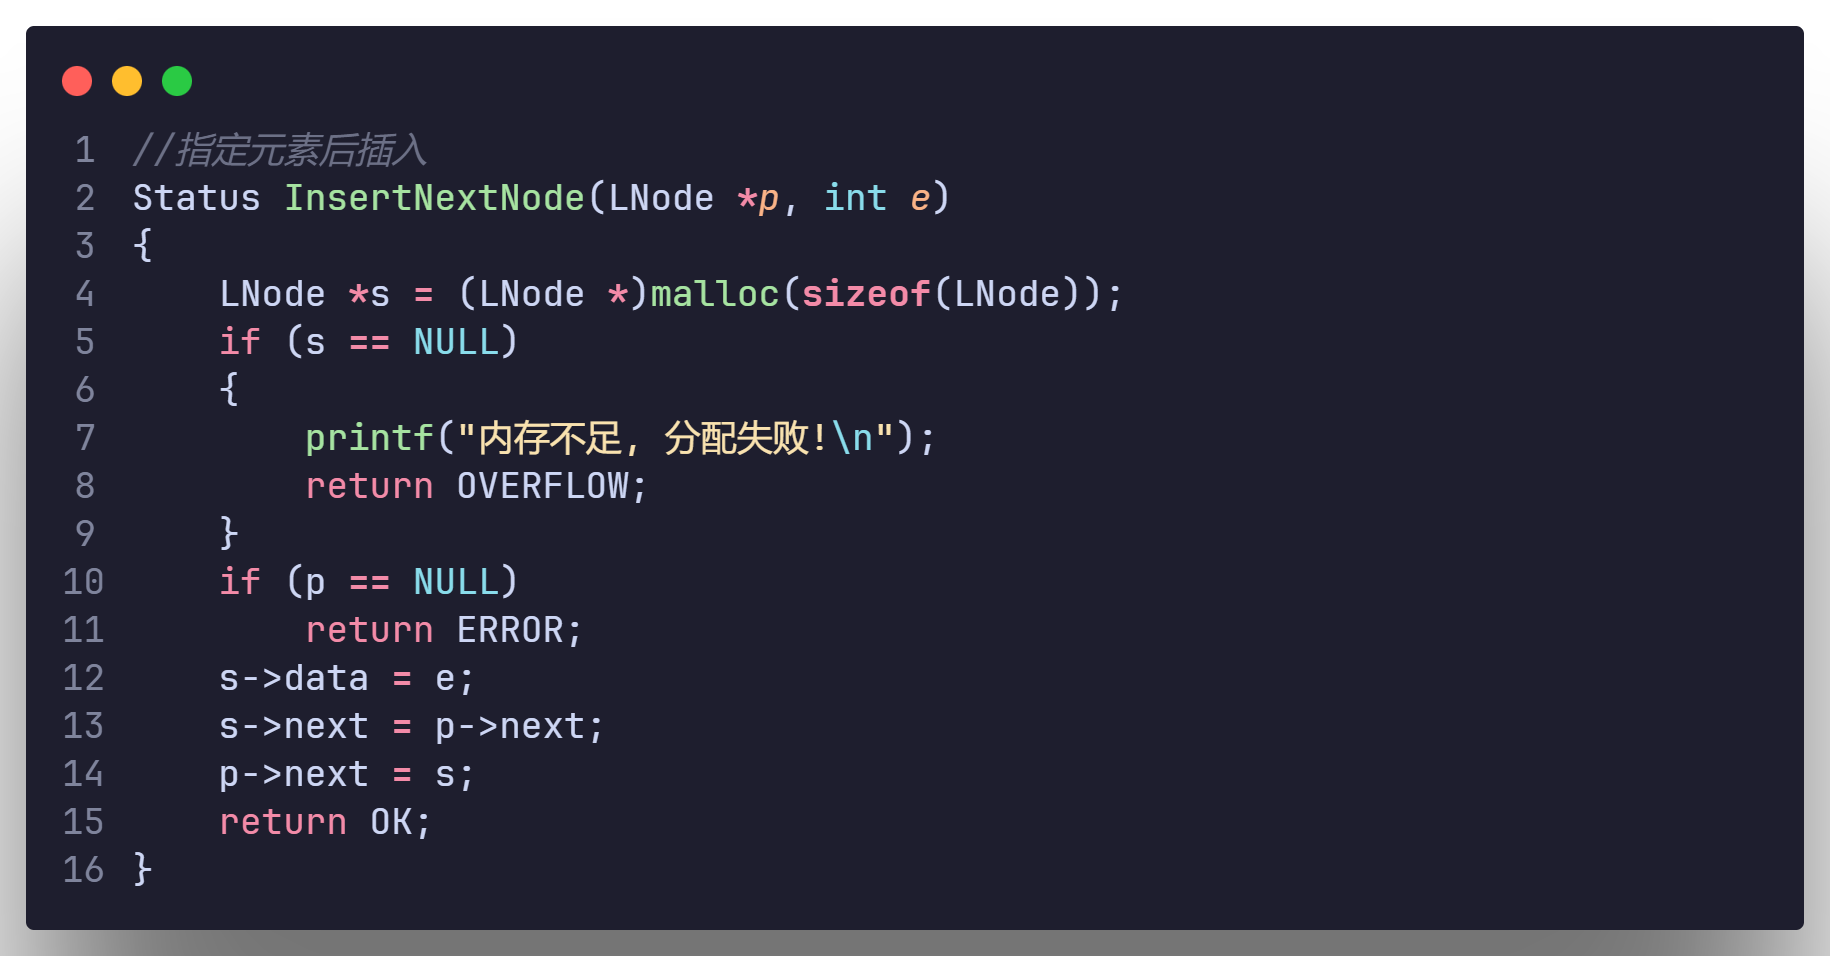
\includegraphics[scale=0.2]{"figure/Note/LinearList/SlBInsert.png"}
\end{figure}

(2). 指定元素前插入

\begin{figure}[H]
    \centering
    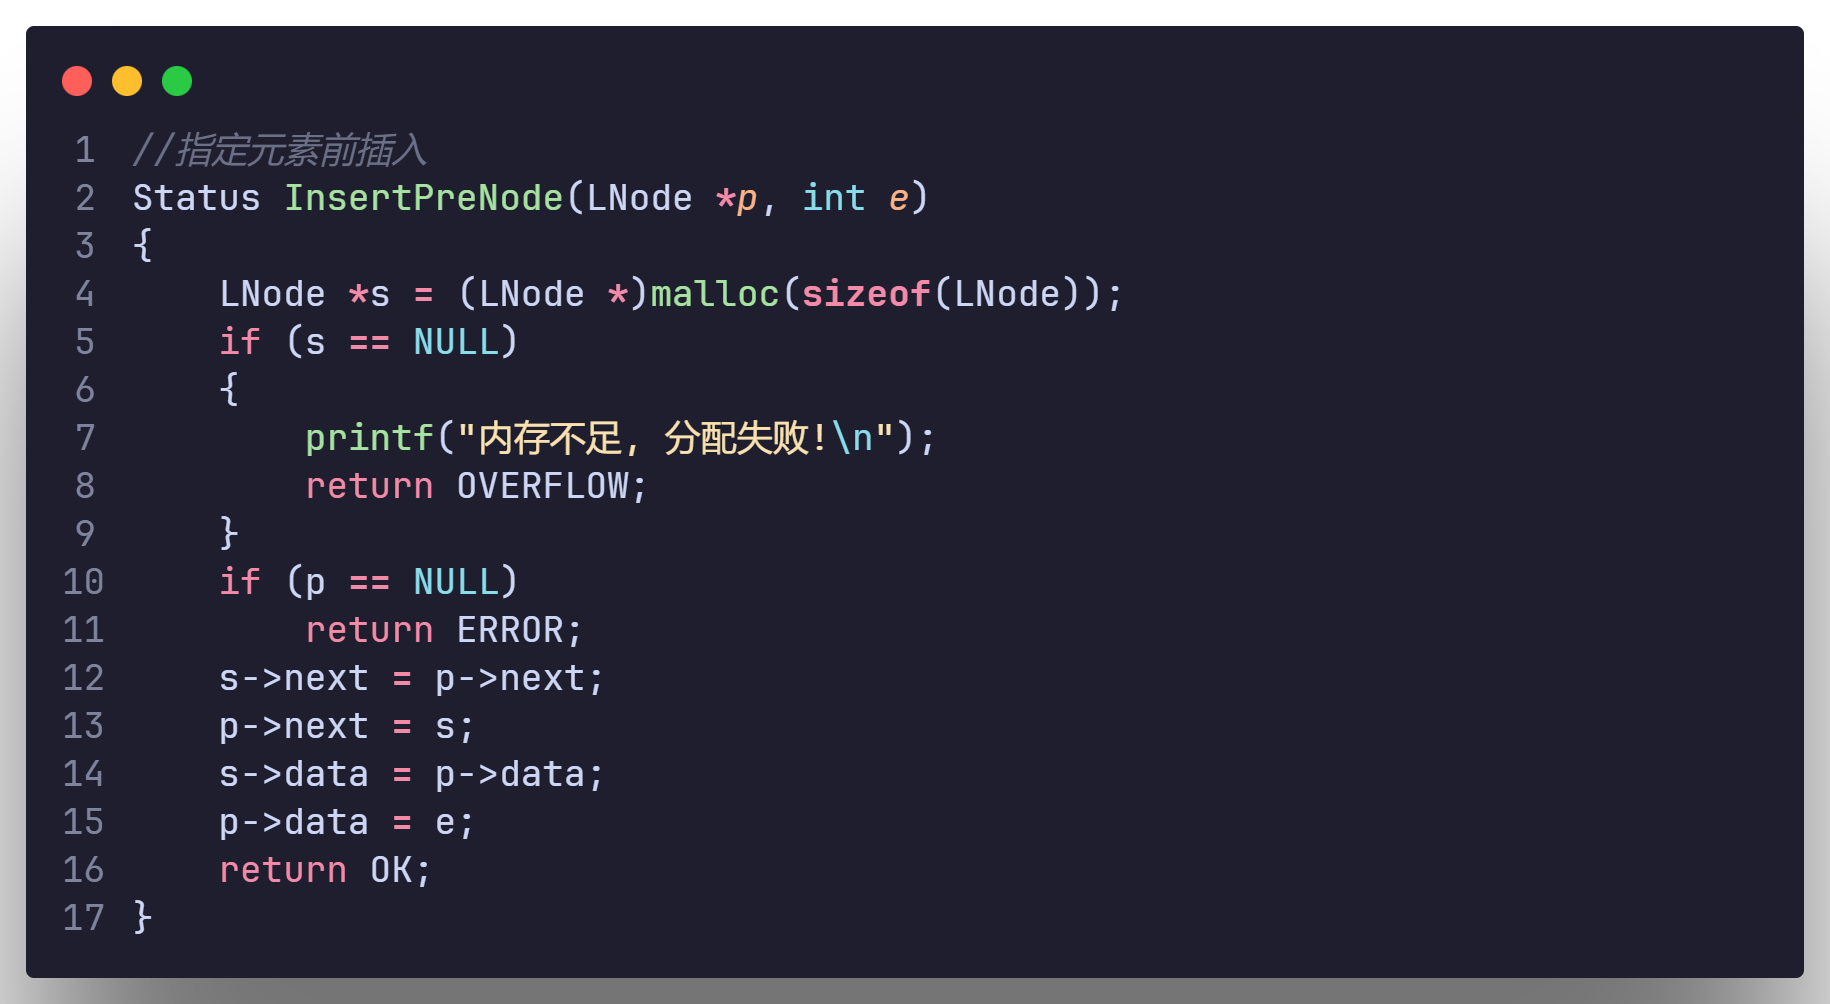
\includegraphics[scale=0.2]{"figure/Note/LinearList/SlFInsert.png"}
\end{figure}

(3). 按位置插入

\begin{figure}[H]
    \centering
    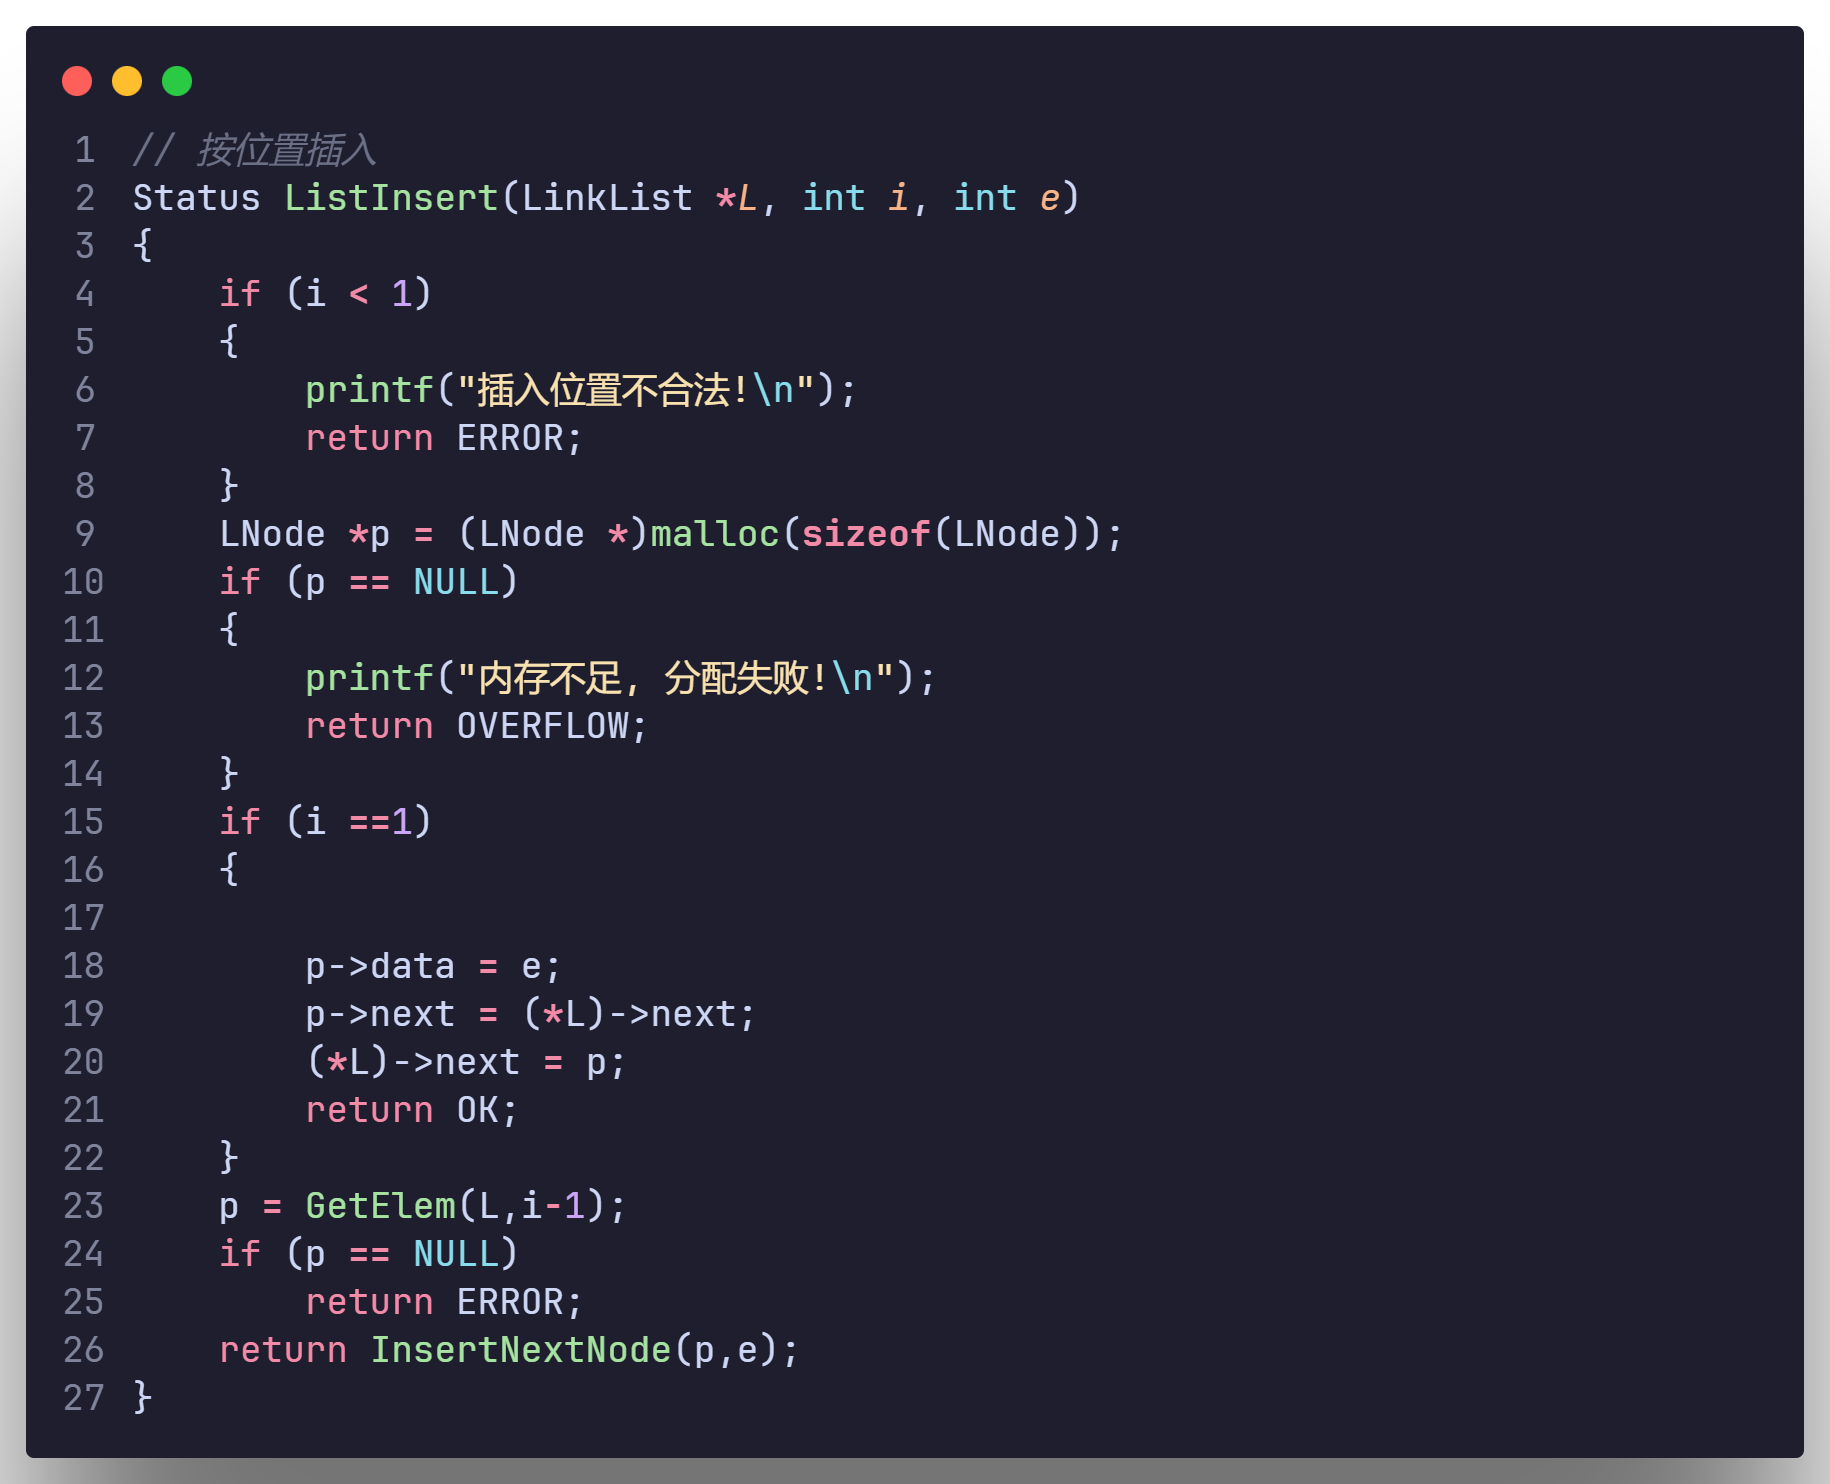
\includegraphics[scale=0.2]{"figure/Note/LinearList/SlInsert.png"}
\end{figure}

\subsubsection{单链表删除}

\begin{figure}[H]
    \centering
    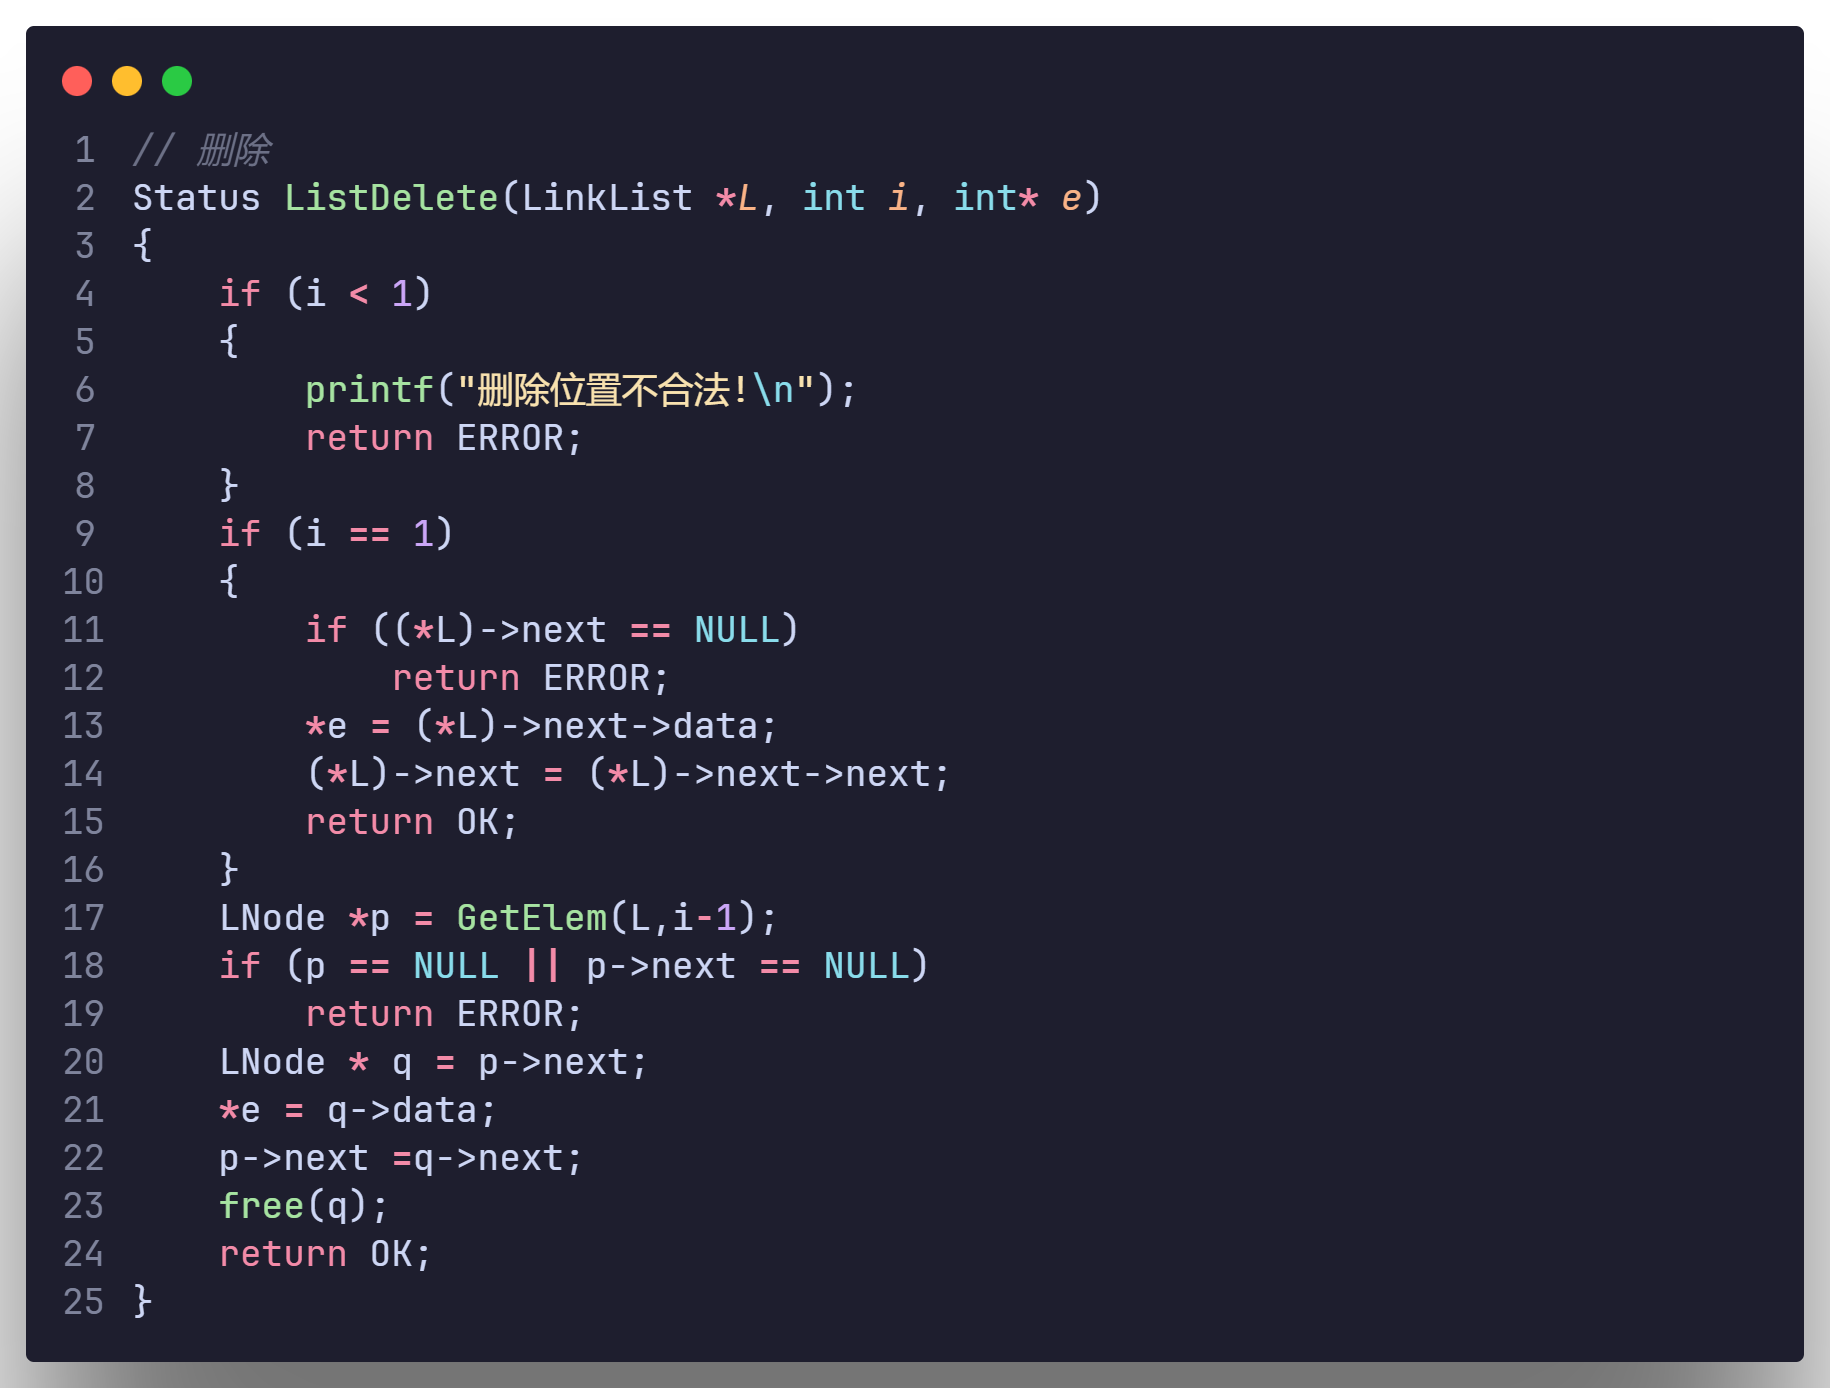
\includegraphics[scale=0.2]{"figure/Note/LinearList/SlDel.png"}
\end{figure}

\subsubsection{单链表辅助函数}

(1). $Length$

\begin{figure}[H]
    \centering
    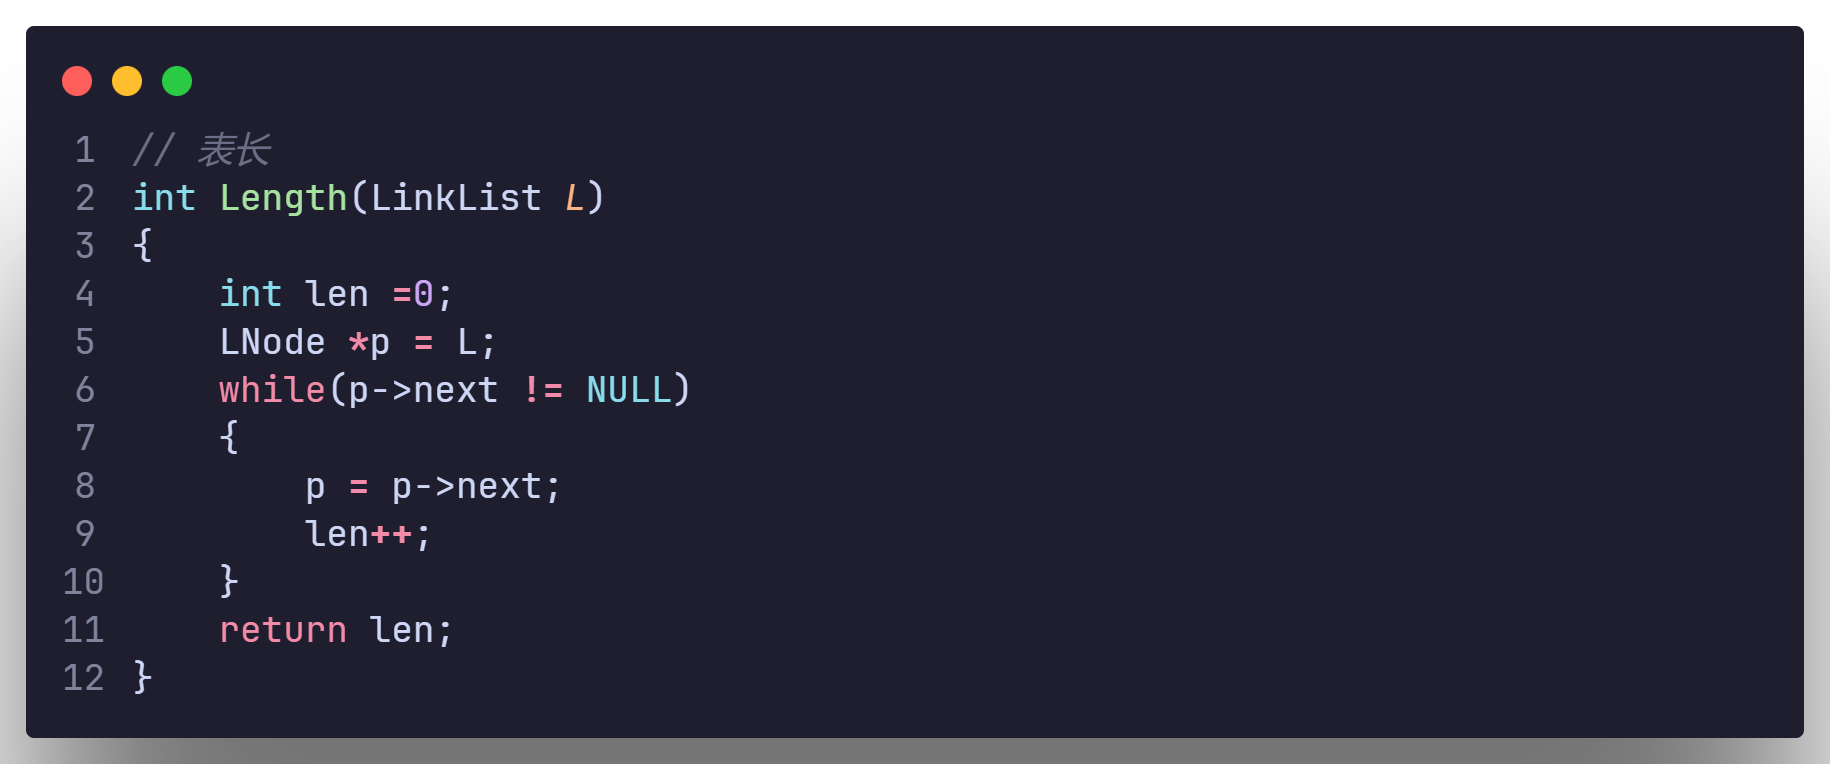
\includegraphics[scale=0.2]{"figure/Note/LinearList/SlLen.png"}
\end{figure}

(2). $Empty$

\begin{figure}[H]
    \centering
    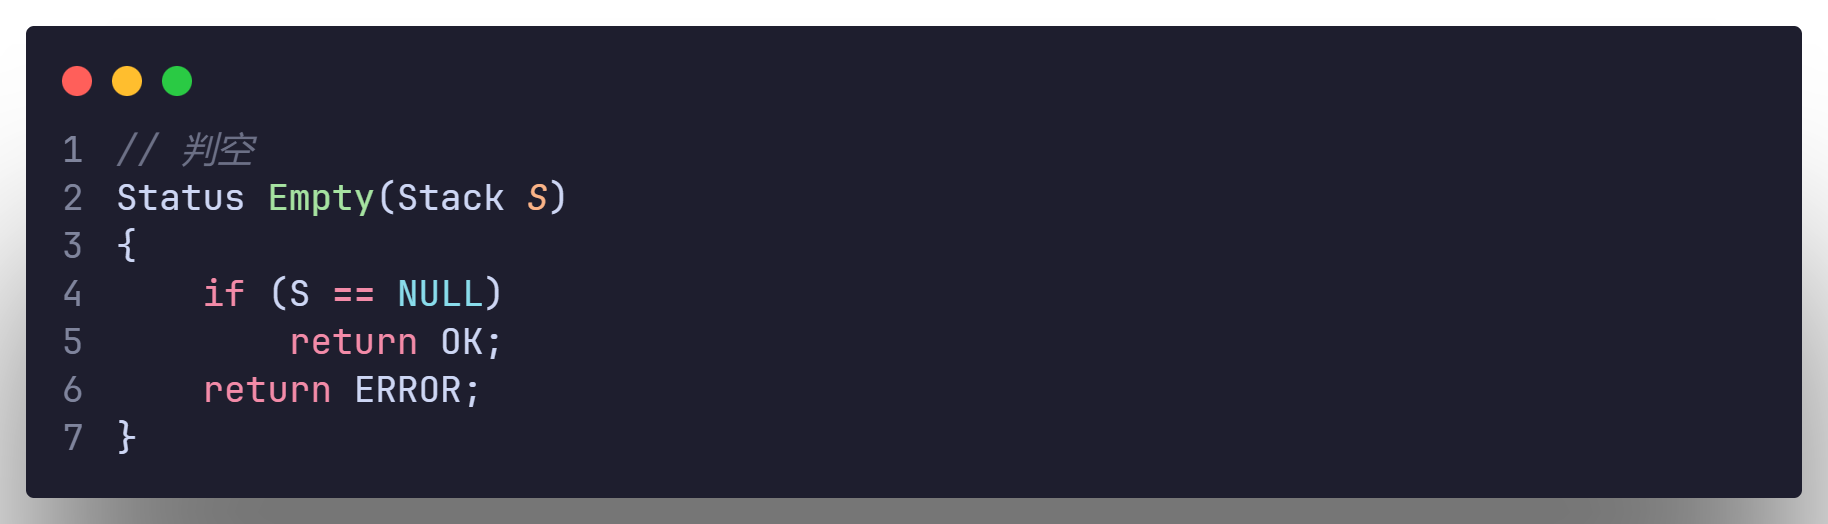
\includegraphics[scale=0.2]{"figure/Note/LinearList/SlEmpty.png"}
\end{figure}

(3). $PrintList$

\begin{figure}[H]
    \centering
    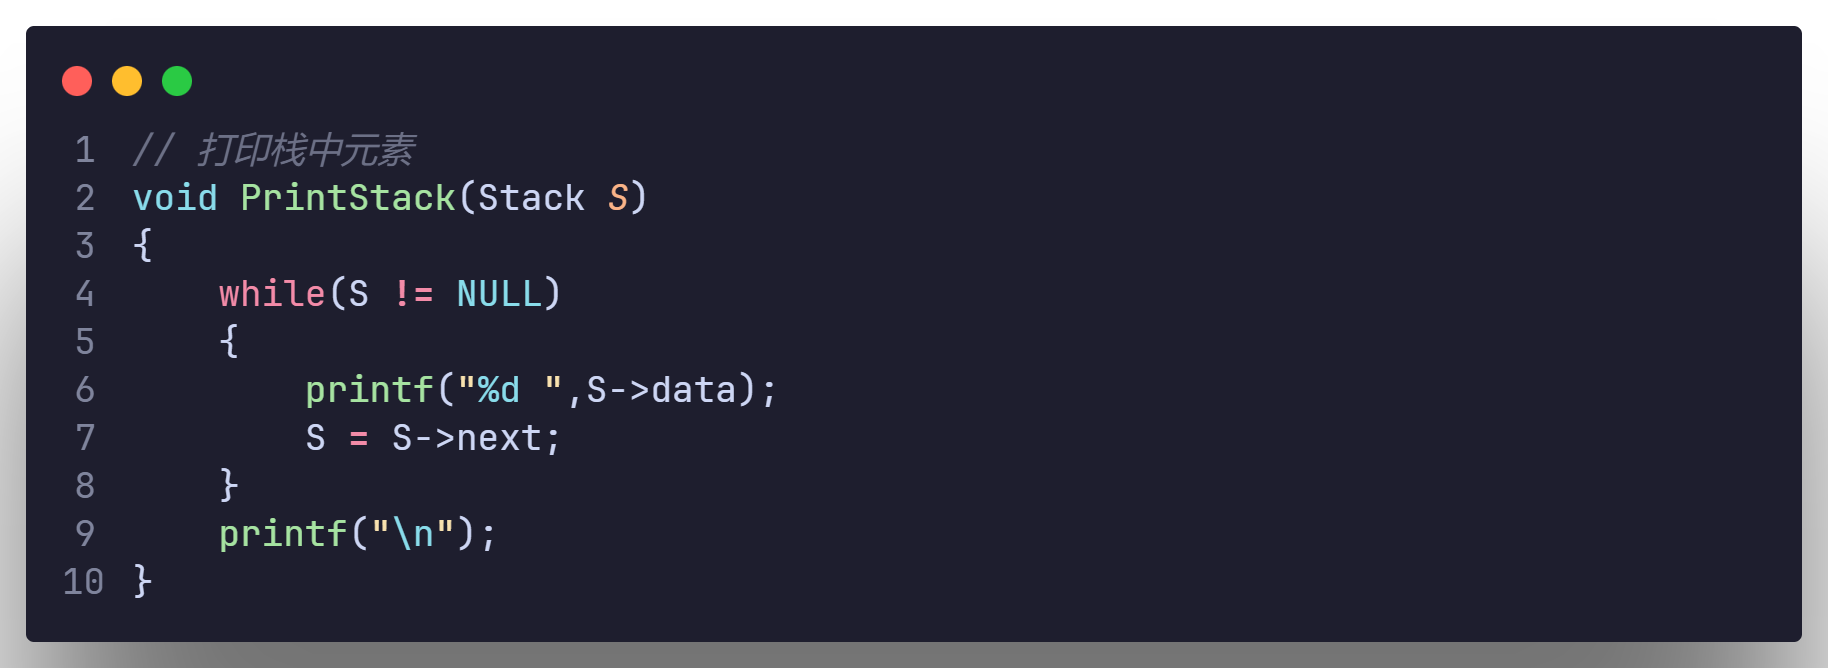
\includegraphics[scale=0.2]{"figure/Note/LinearList/SlPrint.png"}
\end{figure}


\subsubsection{头插法 \& 尾插法}

(1). 头插法

\begin{figure}[H]
    \centering
    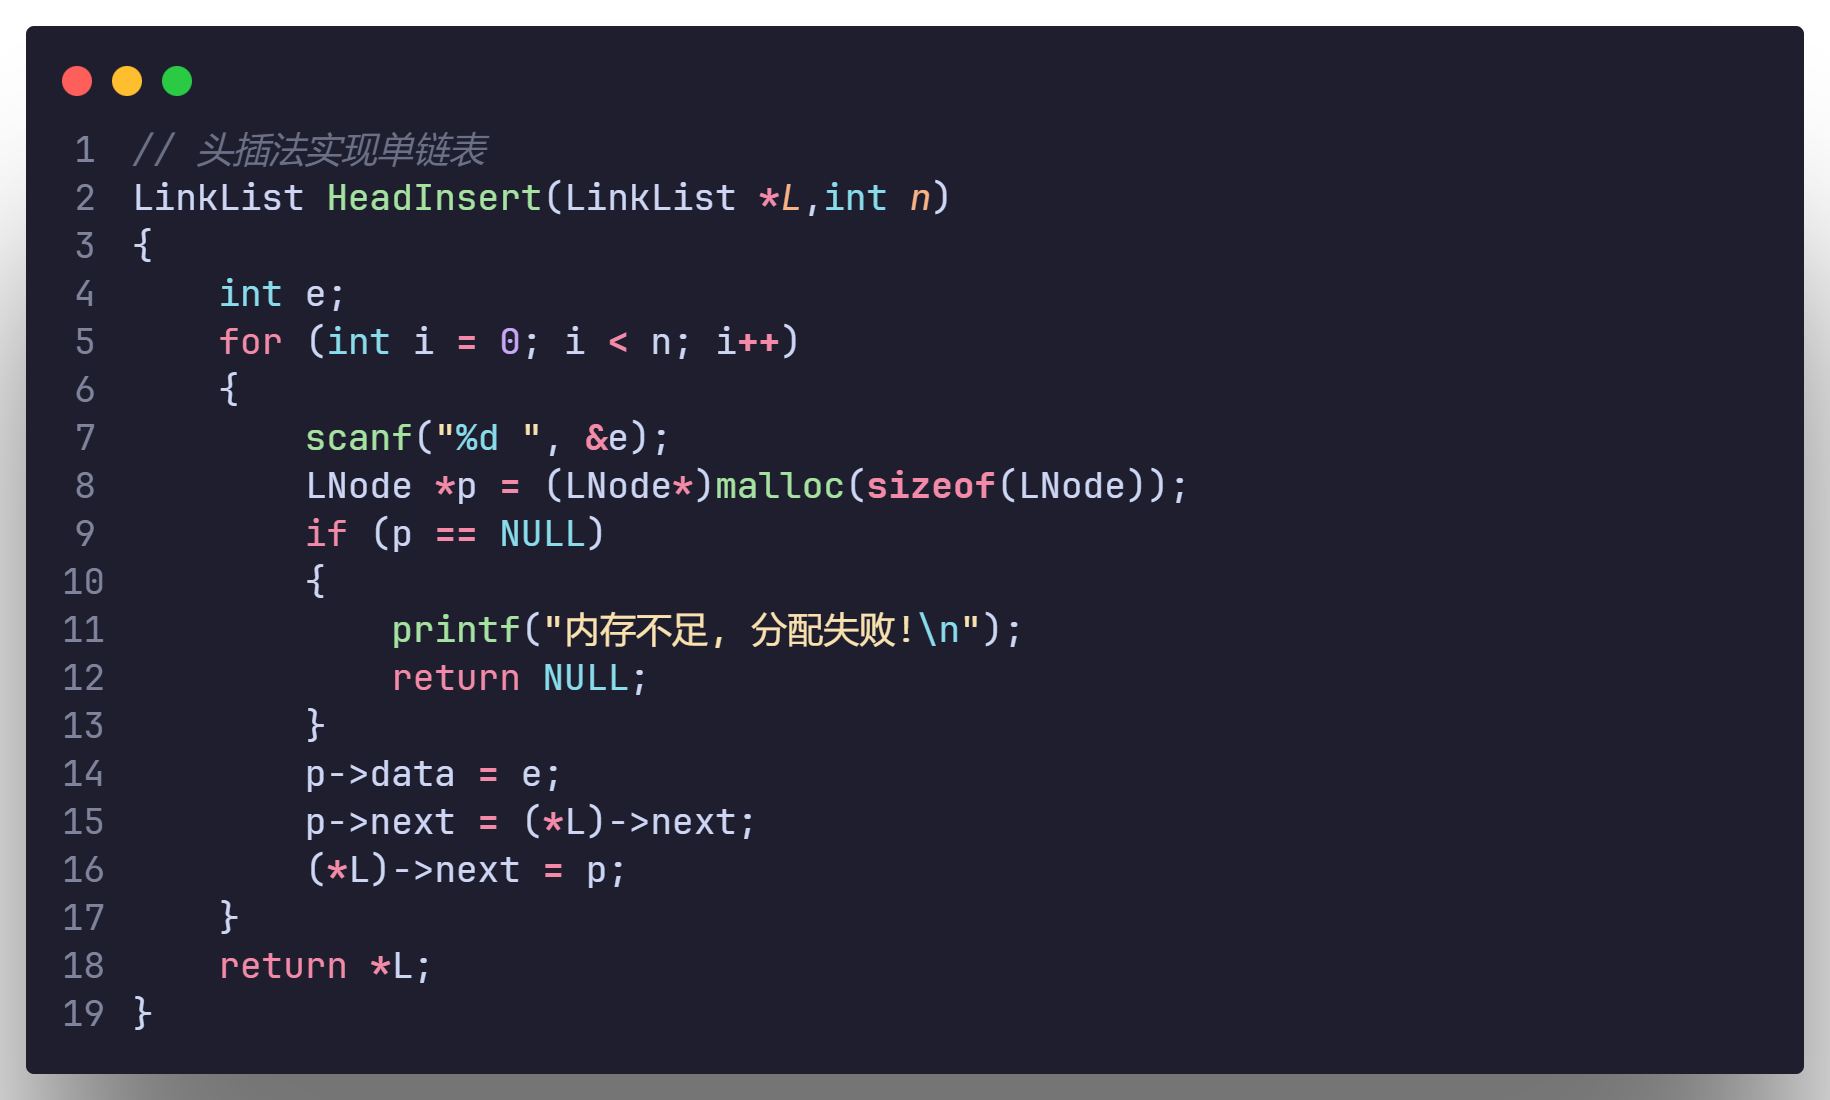
\includegraphics[scale=0.2]{"figure/Note/LinearList/SlHInsert.png"}
\end{figure}

(2). 尾插法

\begin{figure}[H]
    \centering
    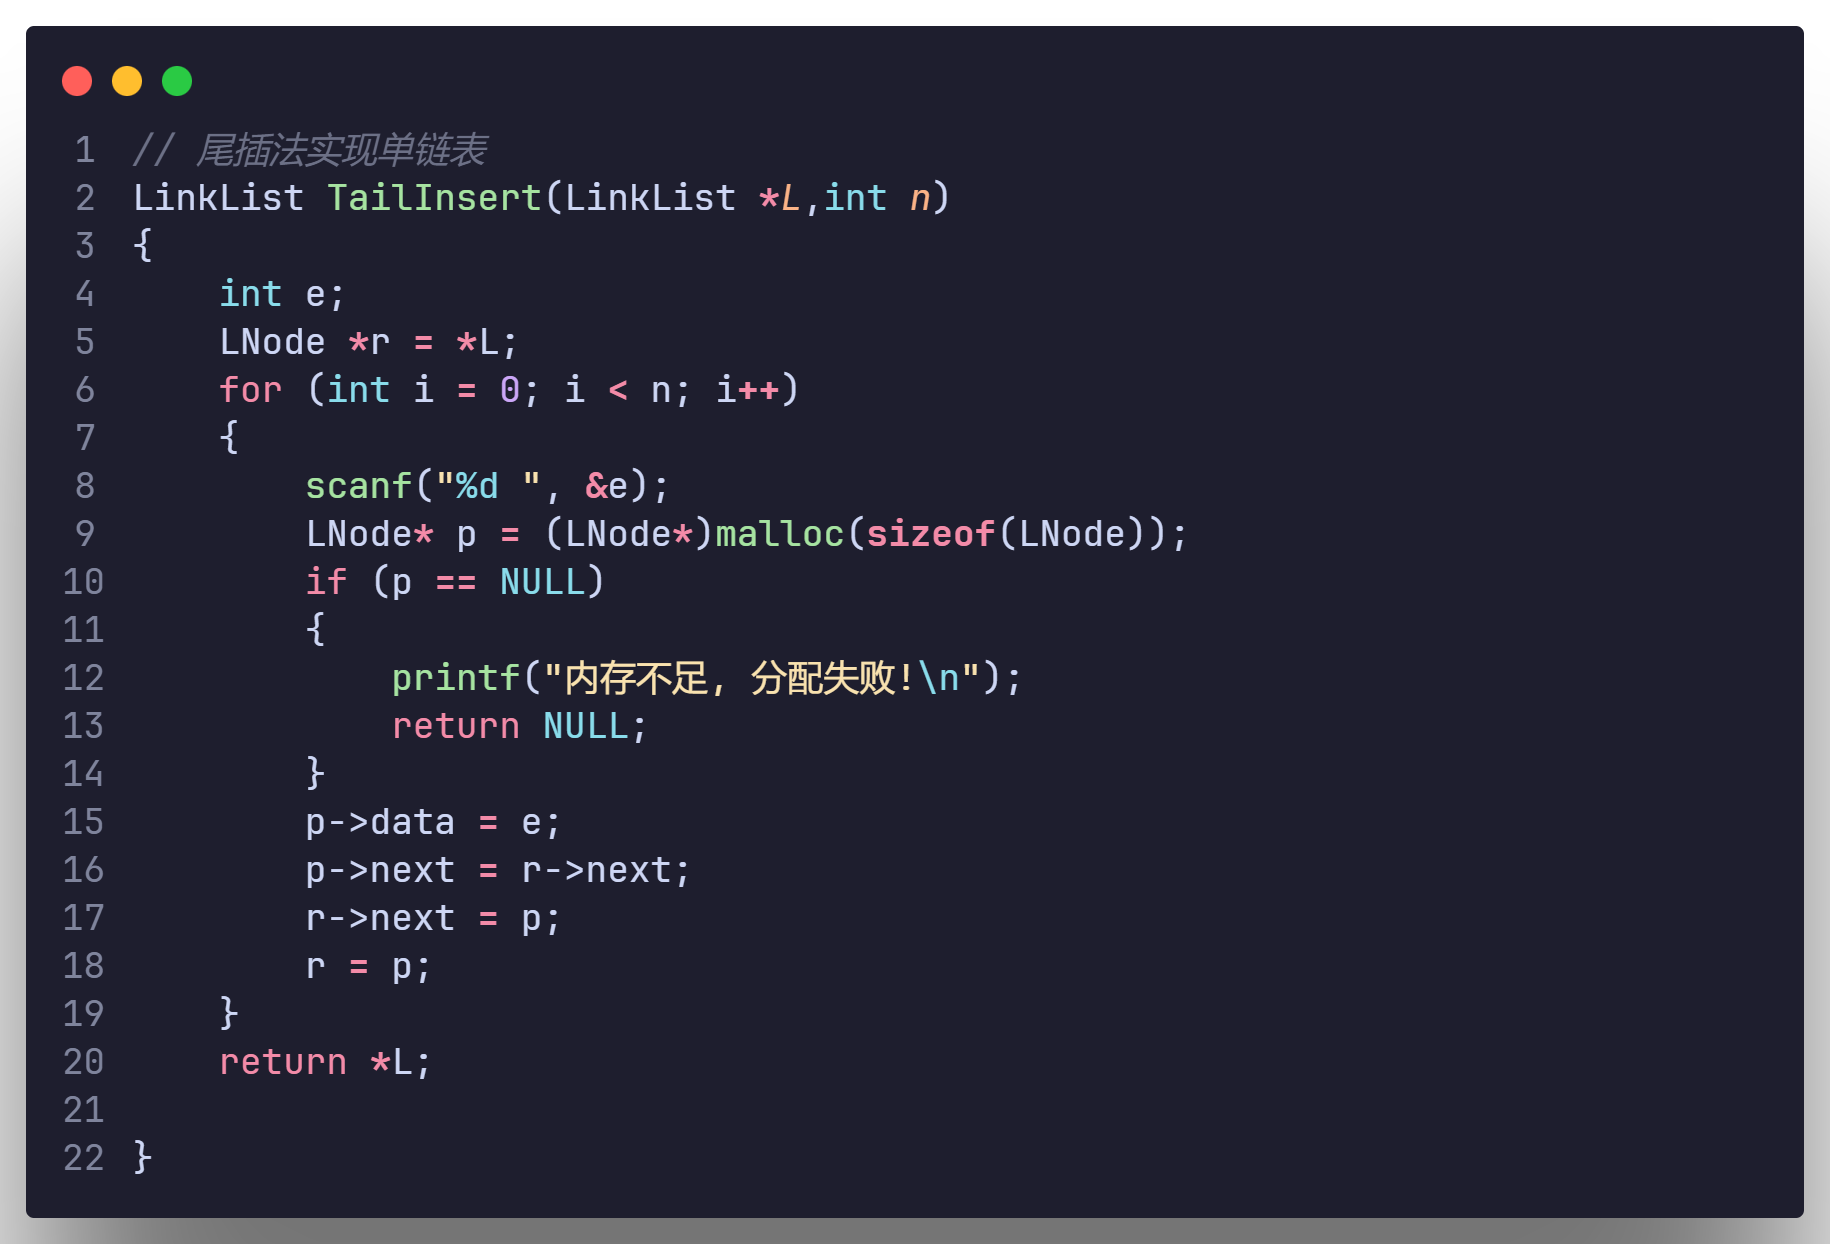
\includegraphics[scale=0.2]{"figure/Note/LinearList/SlTInsert.png"}
\end{figure}

\subsubsection{单链表反转}

\begin{figure}[H]
    \centering
    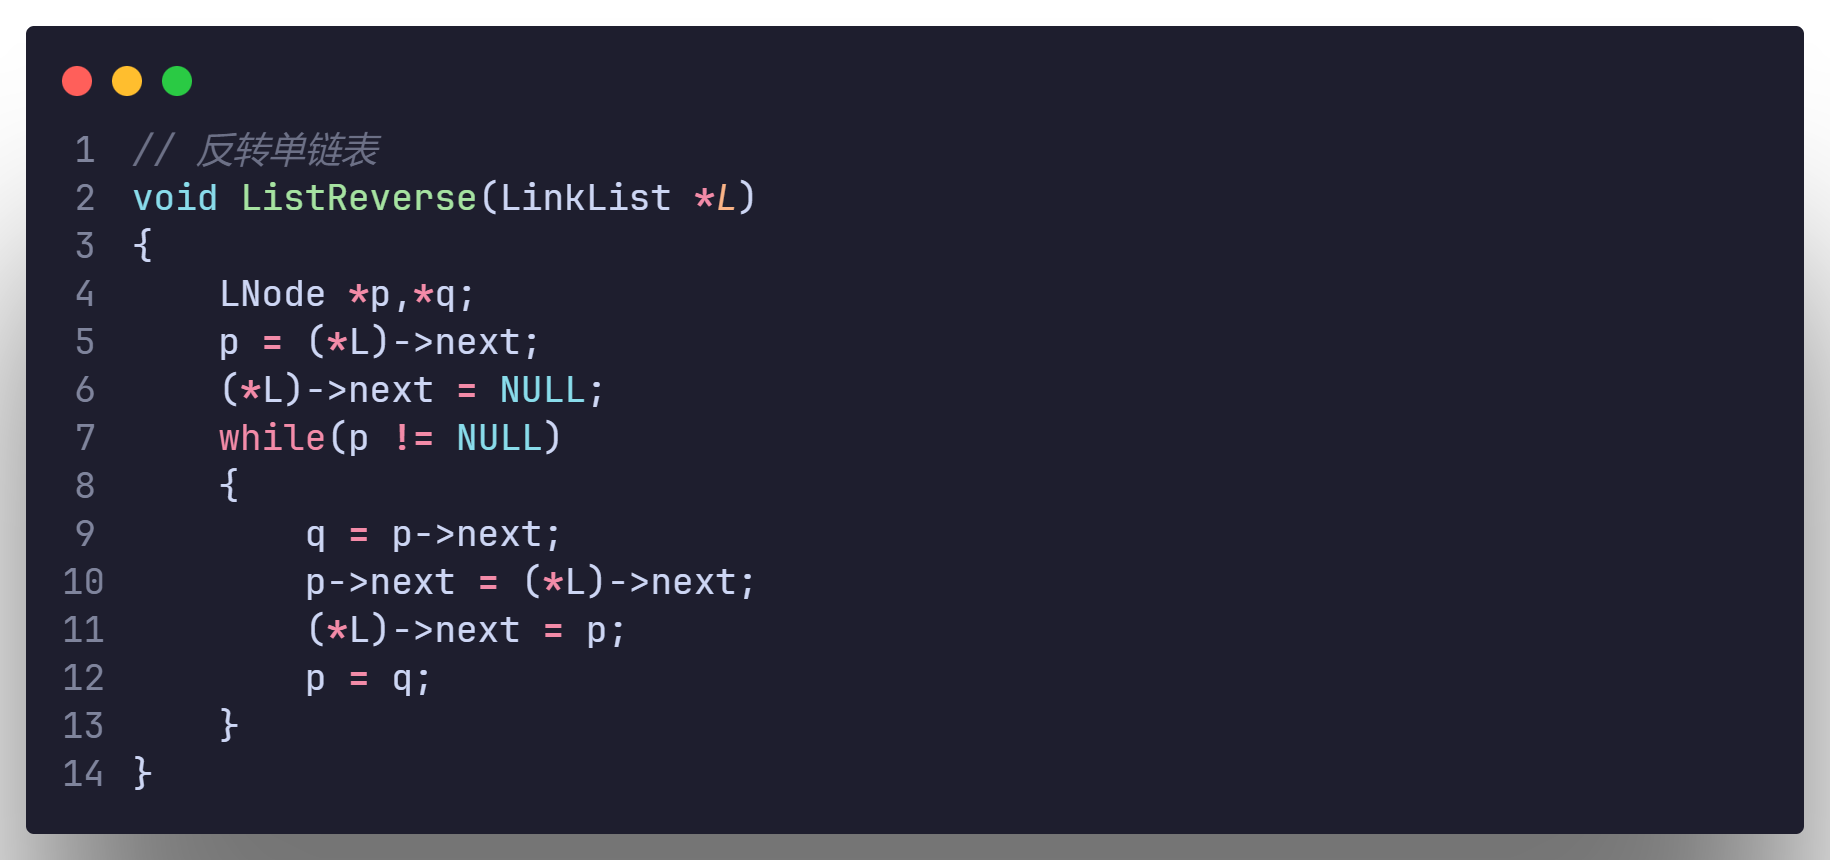
\includegraphics[scale=0.2]{"figure/Note/LinearList/SlReverse.png"}
\end{figure}



\subsection{双链表}
\begin{definition}[双链表]
    \begin{enumerate}
        \item 双链表有两个指针域,分别指向直接前驱和直接后继
        \item 头插法和尾插法的区别, 头插法实现反置
        \item 在插入和删除时,第一个和最后一个节点有特殊情况
    \end{enumerate}
\end{definition}

\subsubsection{双链表定义和函数声明}

\begin{figure}[H]
    \centering
    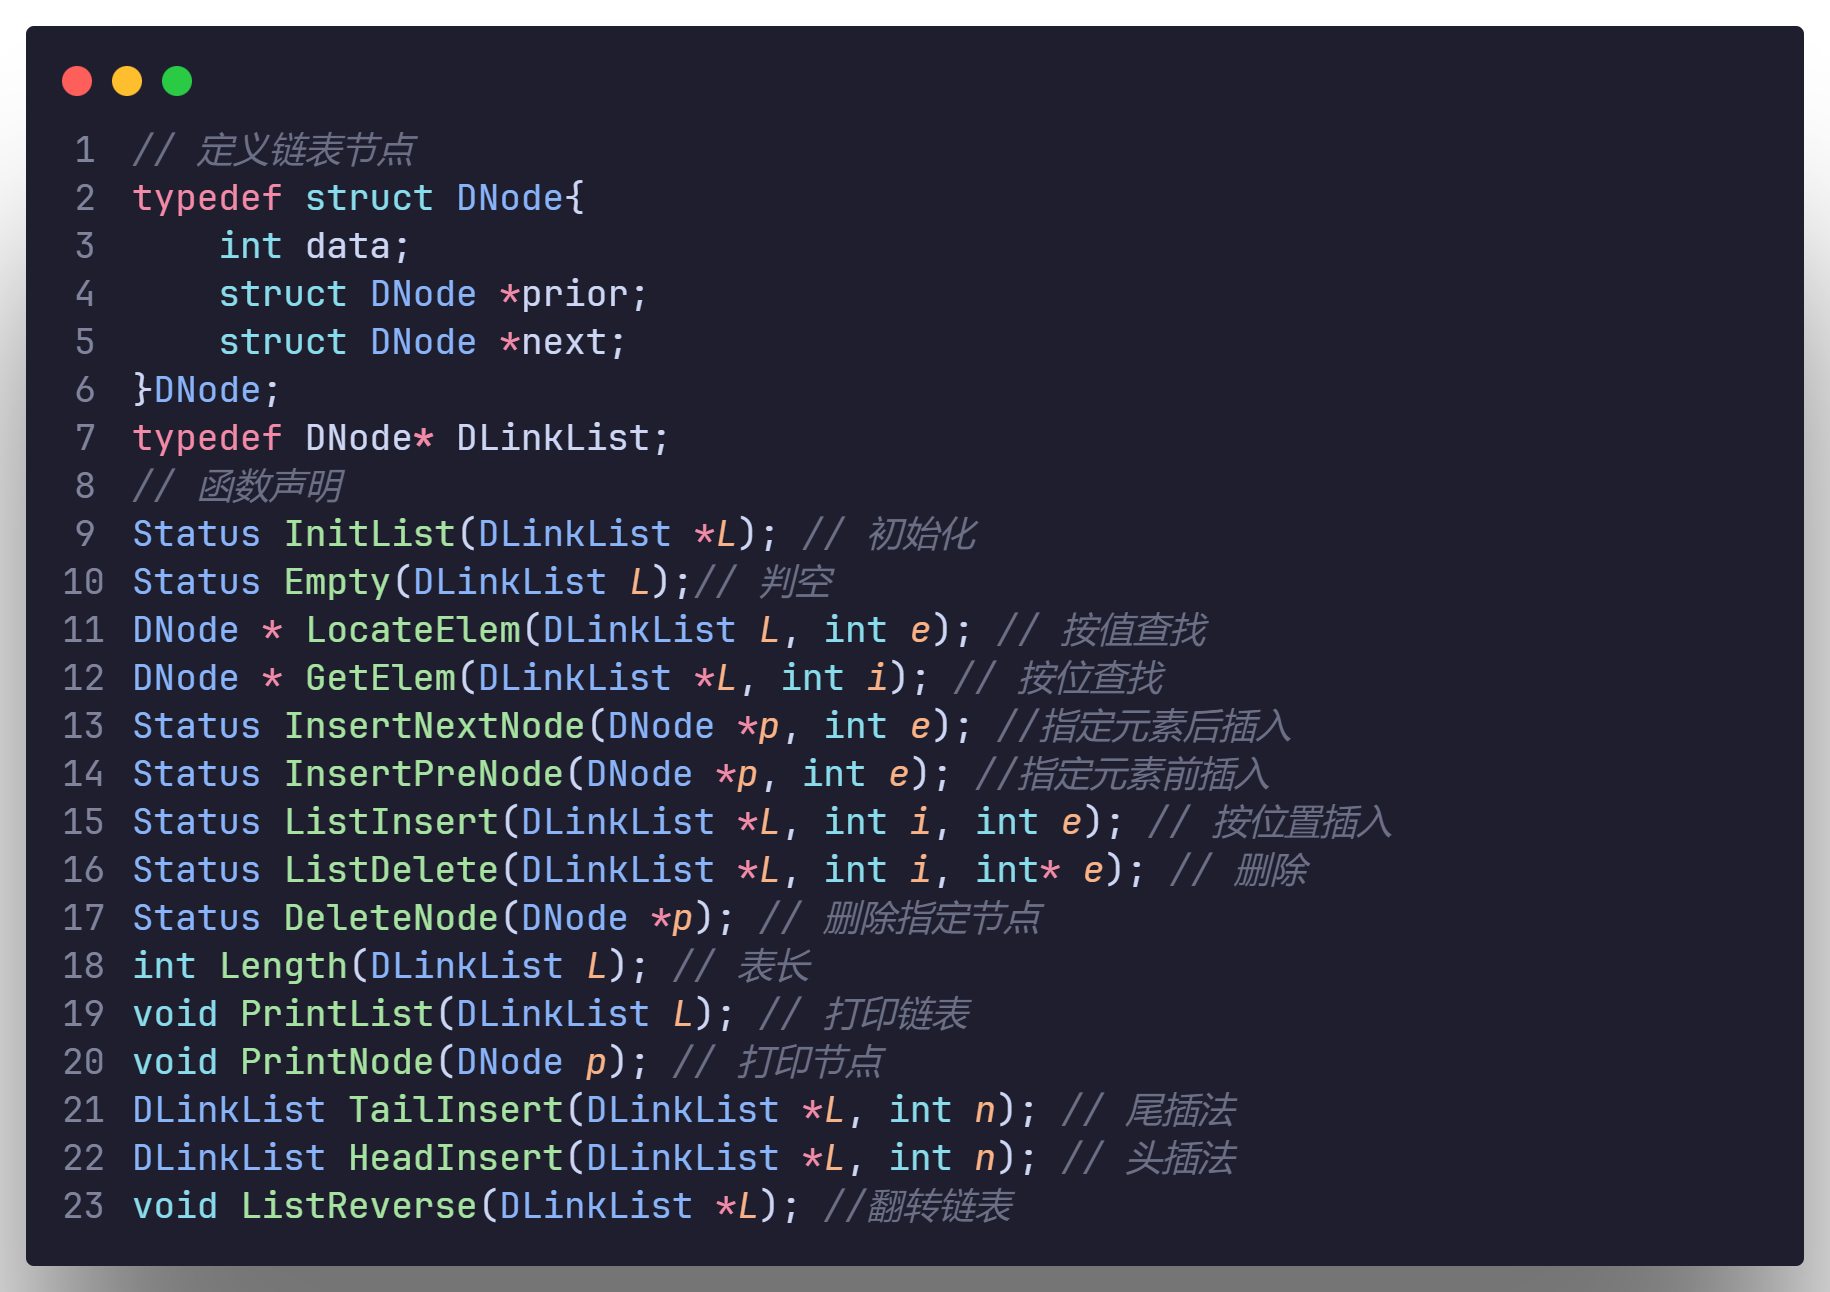
\includegraphics[scale=0.2]{"figure/Note/LinearList/DlFunction.png"}
\end{figure}

\subsubsection{双链表初始化}

\begin{figure}[H]
    \centering
    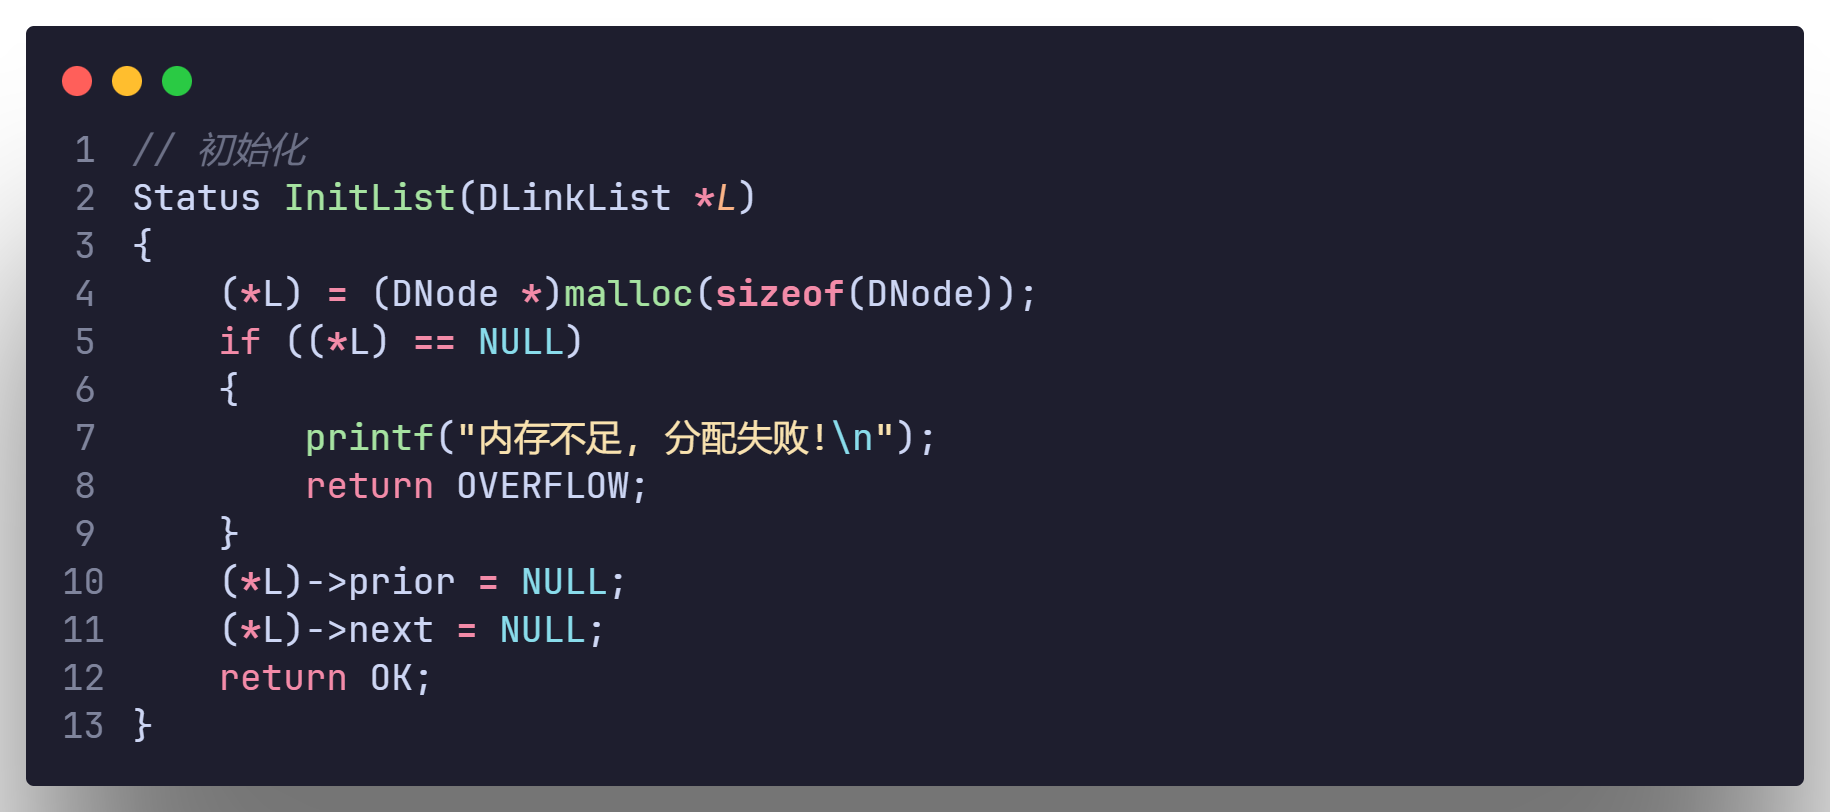
\includegraphics[scale=0.2]{"figure/Note/LinearList/DlInit.png"}
\end{figure}

\subsubsection{双链表查找}

(1). 按位置查找

\begin{figure}[H]
    \centering
    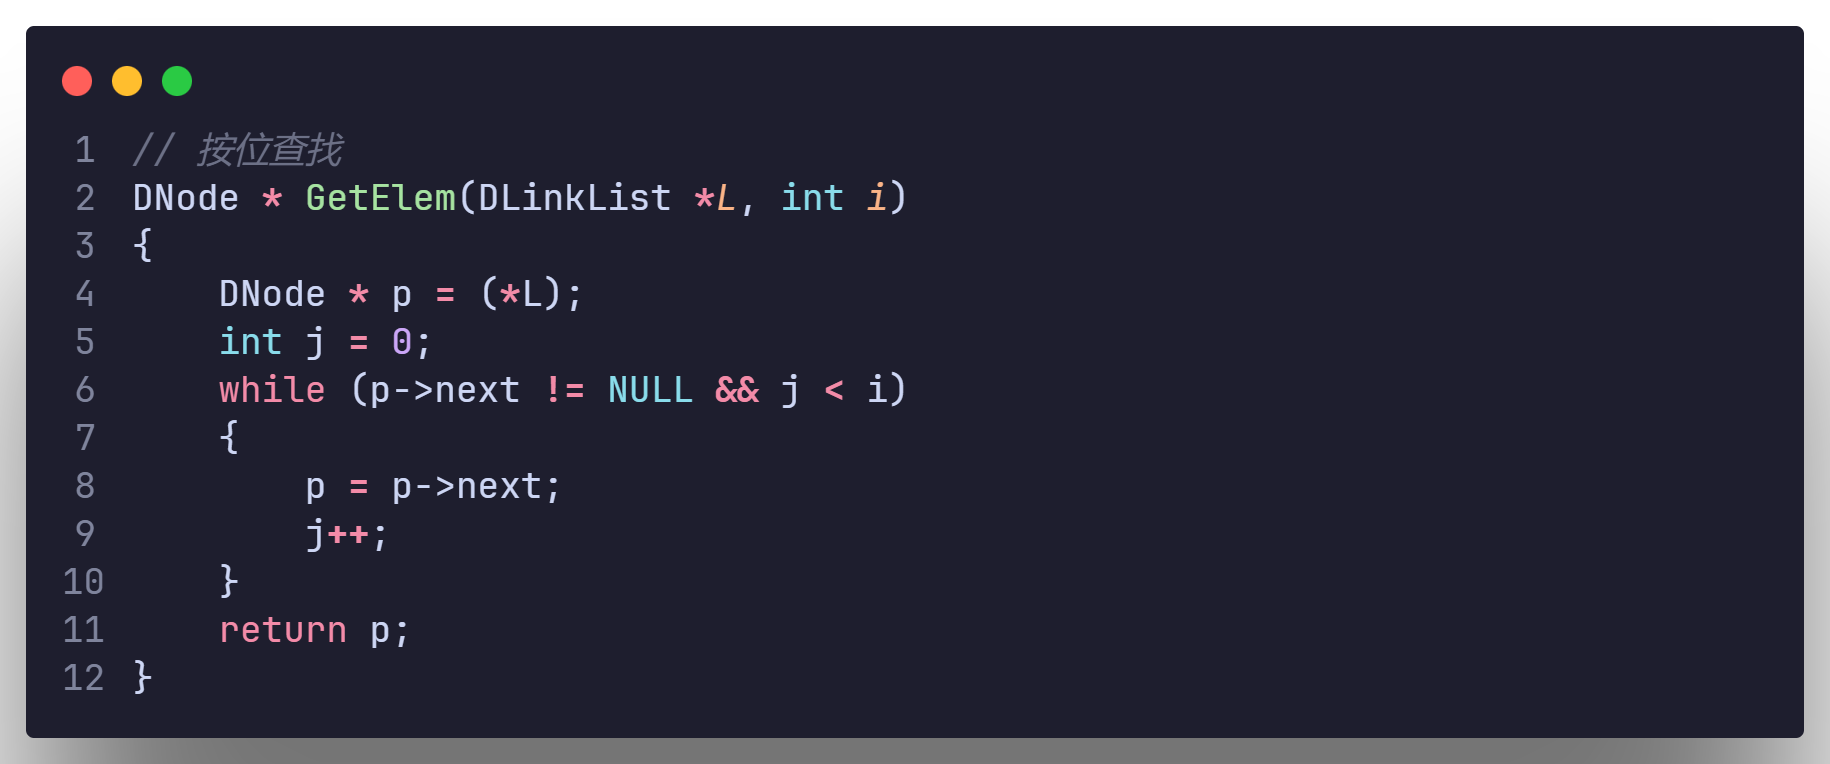
\includegraphics[scale=0.2]{"figure/Note/LinearList/DlNumSer.png"}
\end{figure}

(2). 按值查找

\begin{figure}[H]
    \centering
    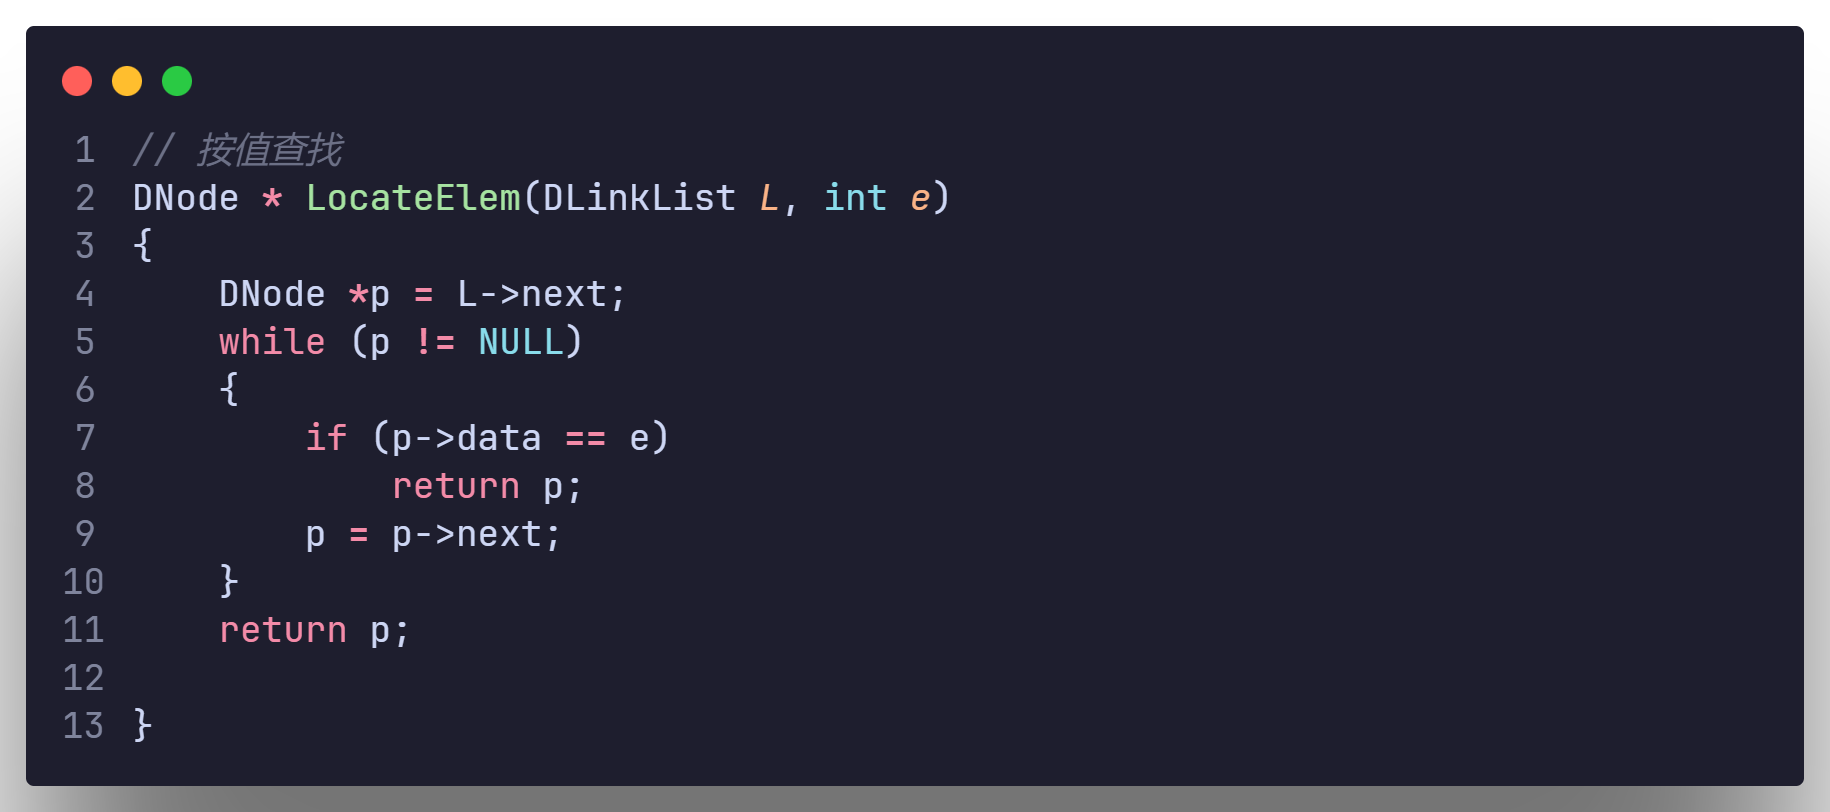
\includegraphics[scale=0.2]{"figure/Note/LinearList/DlItemSer.png"}
\end{figure}

\subsubsection{双链表插入}

(1). 指定元素后插入

\begin{figure}[H]
    \centering
    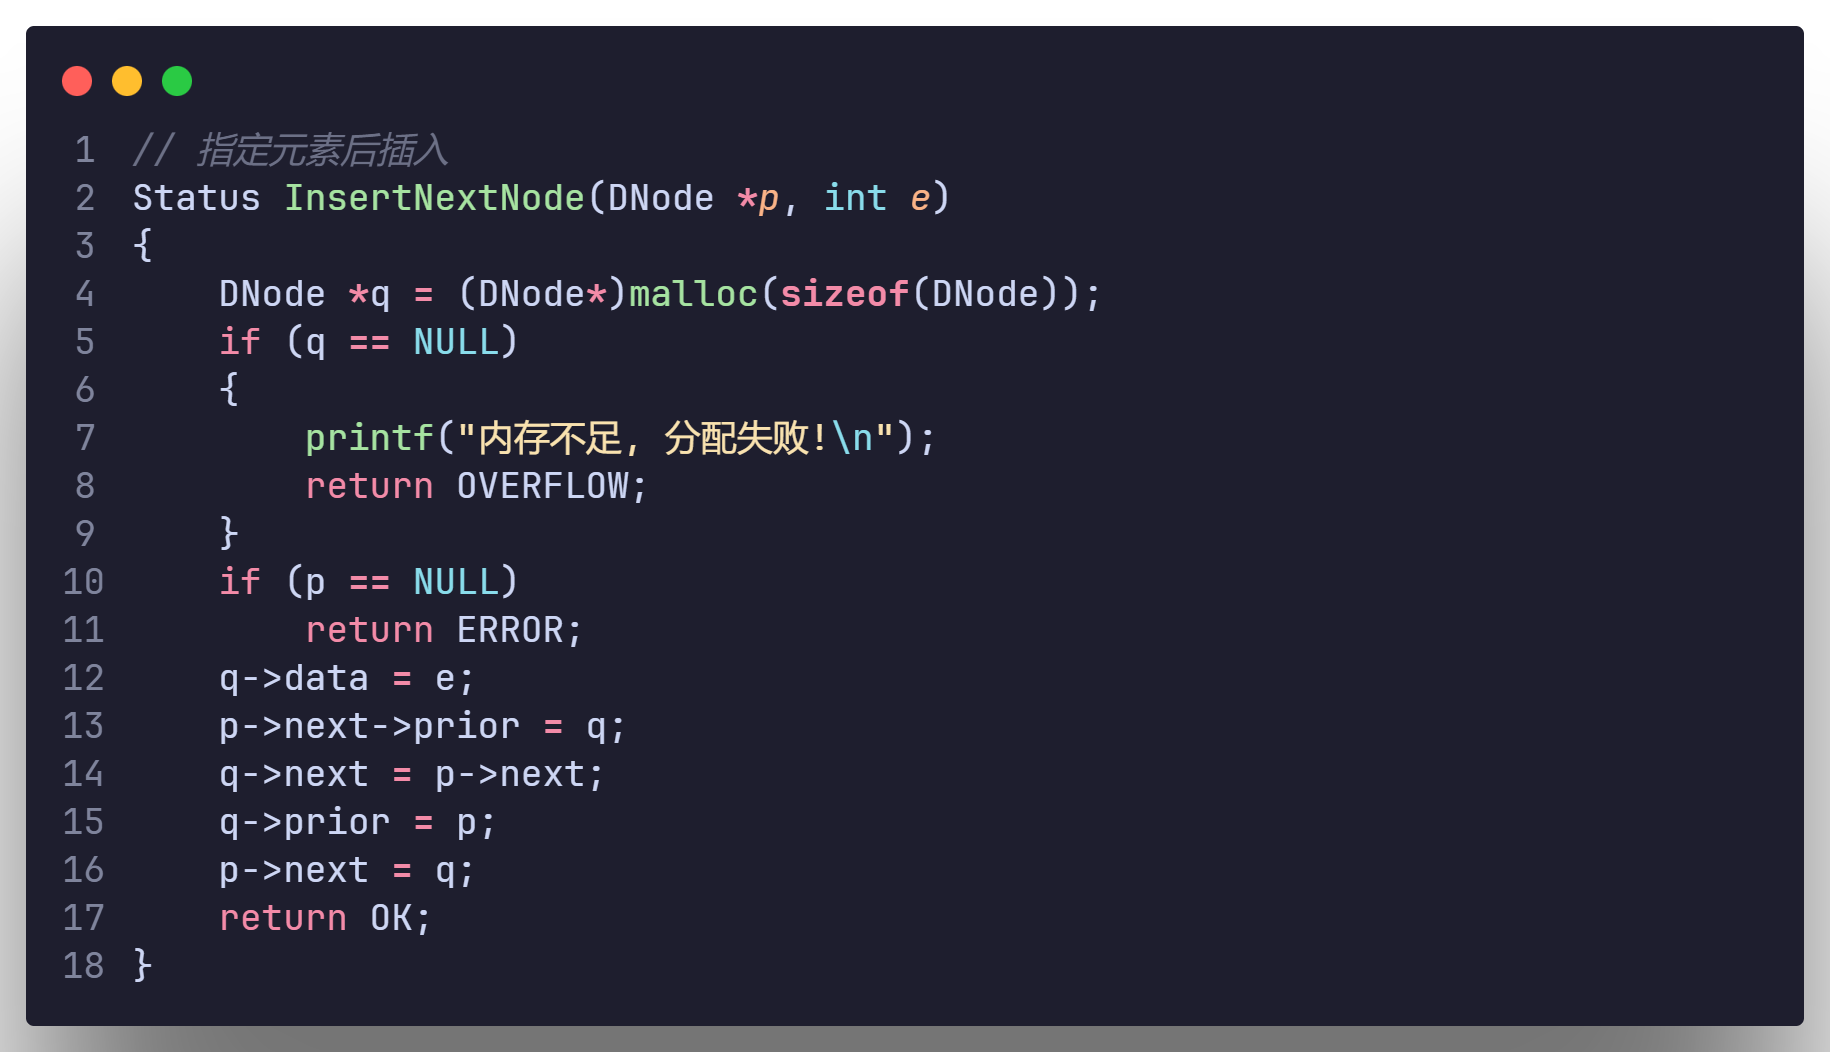
\includegraphics[scale=0.2]{"figure/Note/LinearList/DlBInsert.png"}
\end{figure}

(2). 指定元素前插入

\begin{figure}[H]
    \centering
    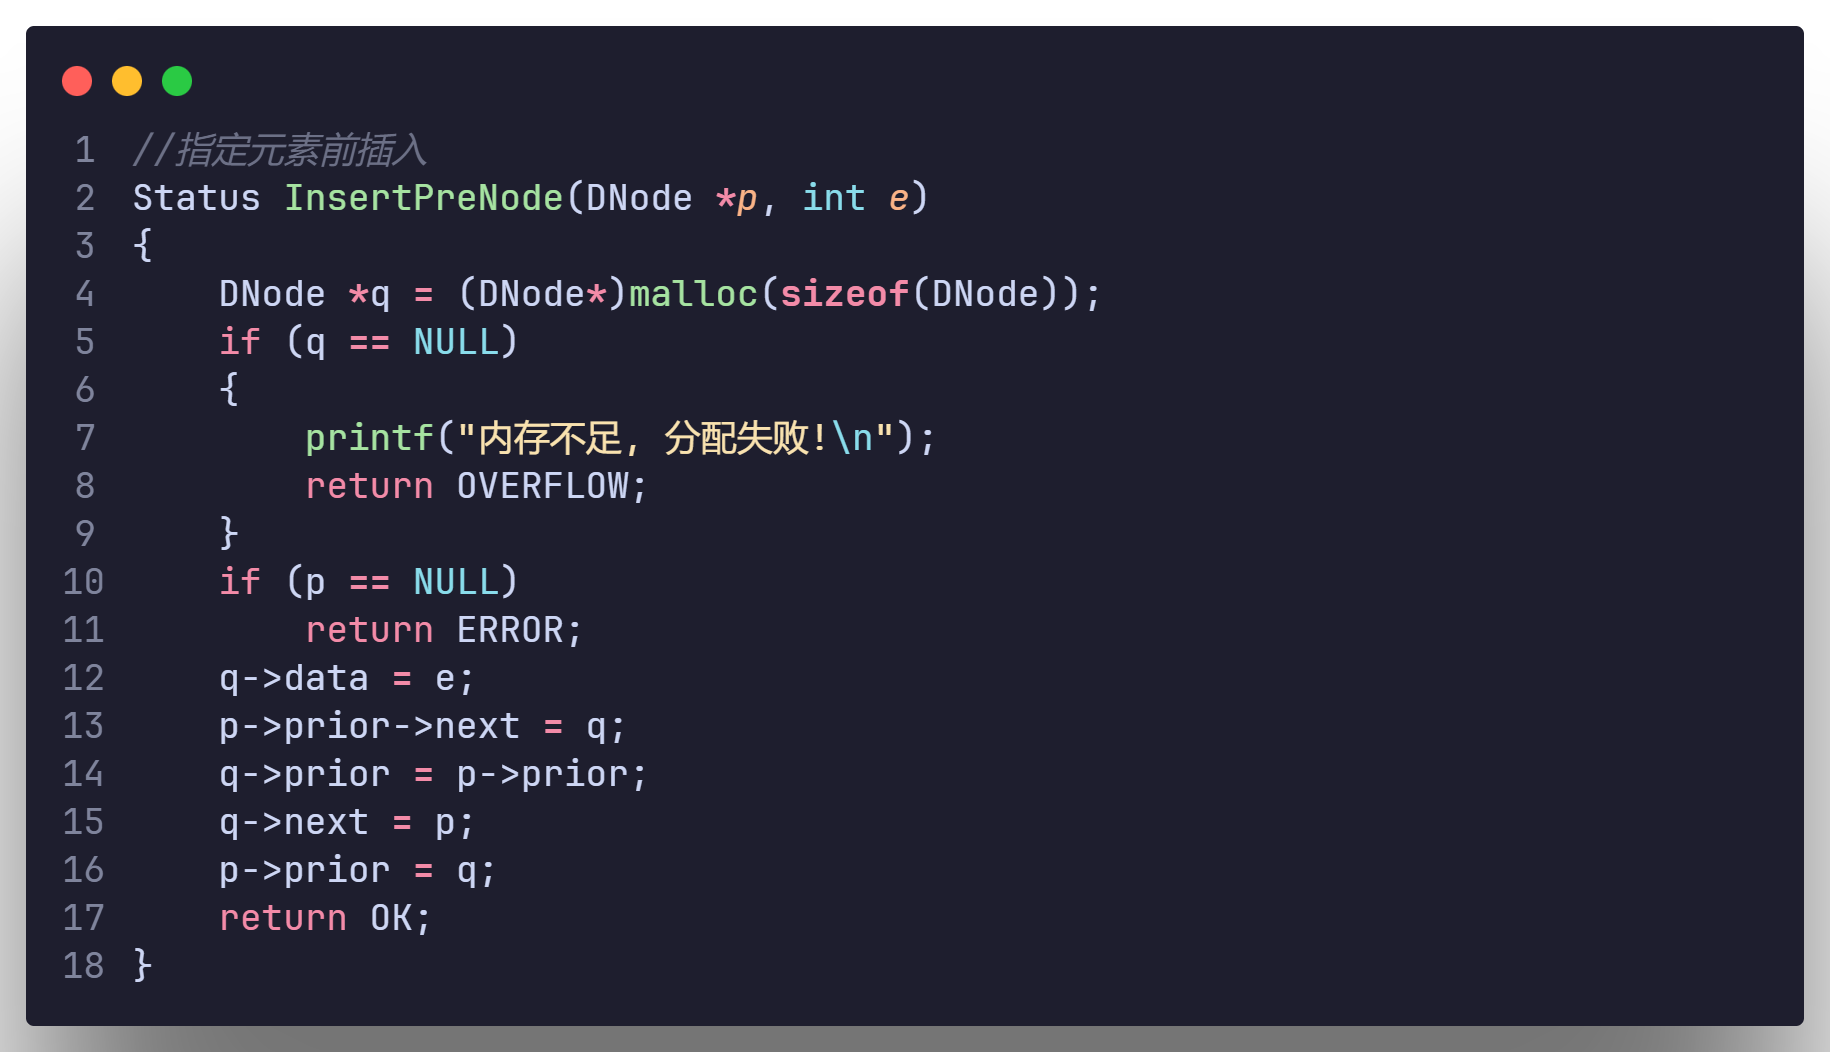
\includegraphics[scale=0.2]{"figure/Note/LinearList/DlFInsert.png"}
\end{figure}

(3). 指定位置插入

\begin{figure}[H]
    \centering
    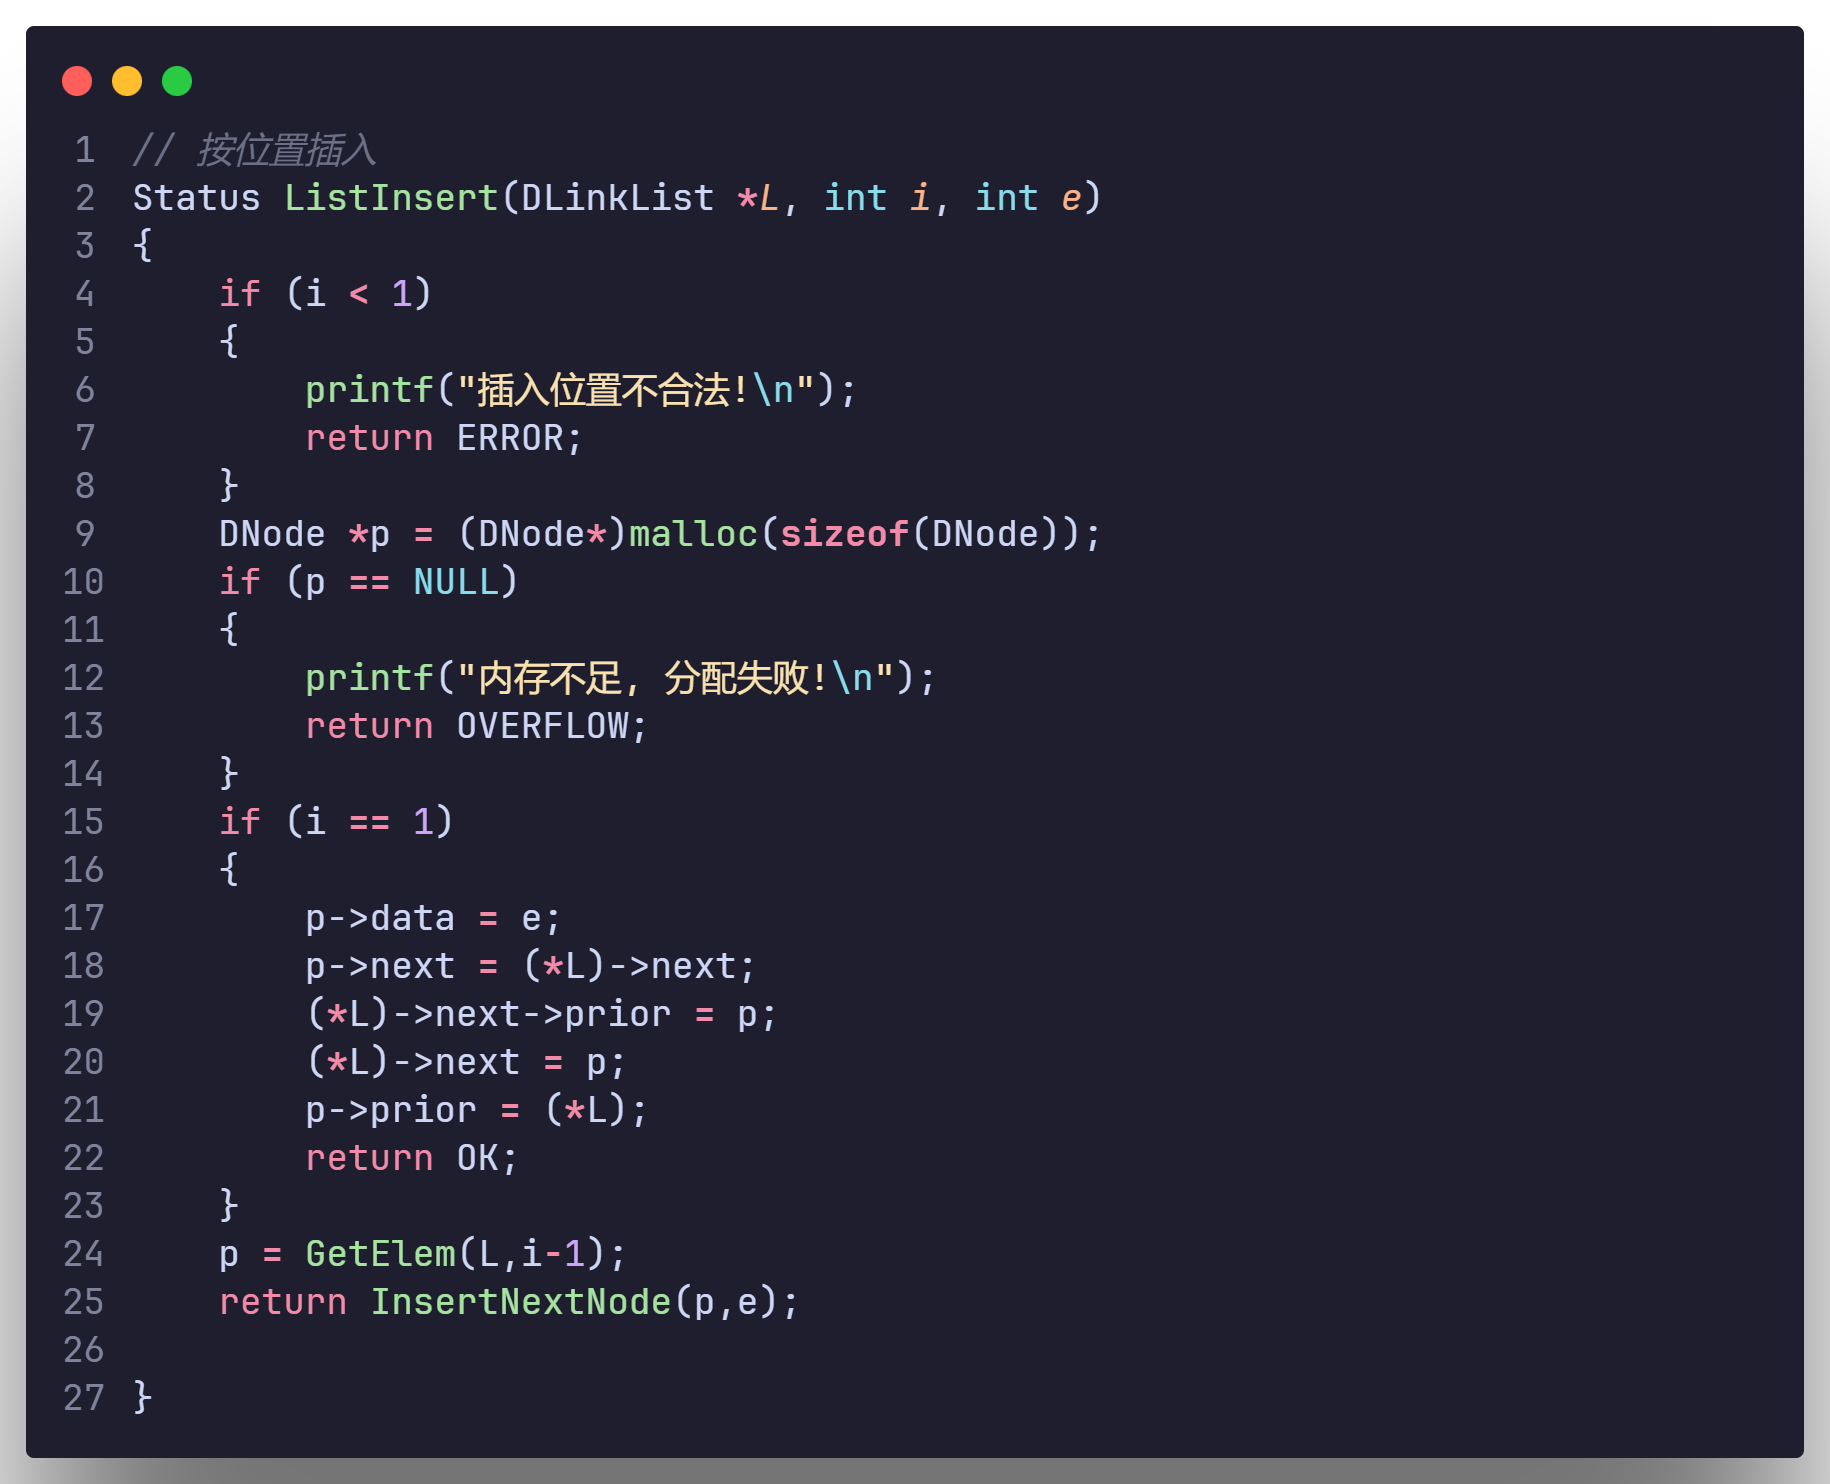
\includegraphics[scale=0.2]{"figure/Note/LinearList/DlInsert.png"}
\end{figure}


\subsubsection{双链表删除}

\begin{figure}[H]
    \centering
    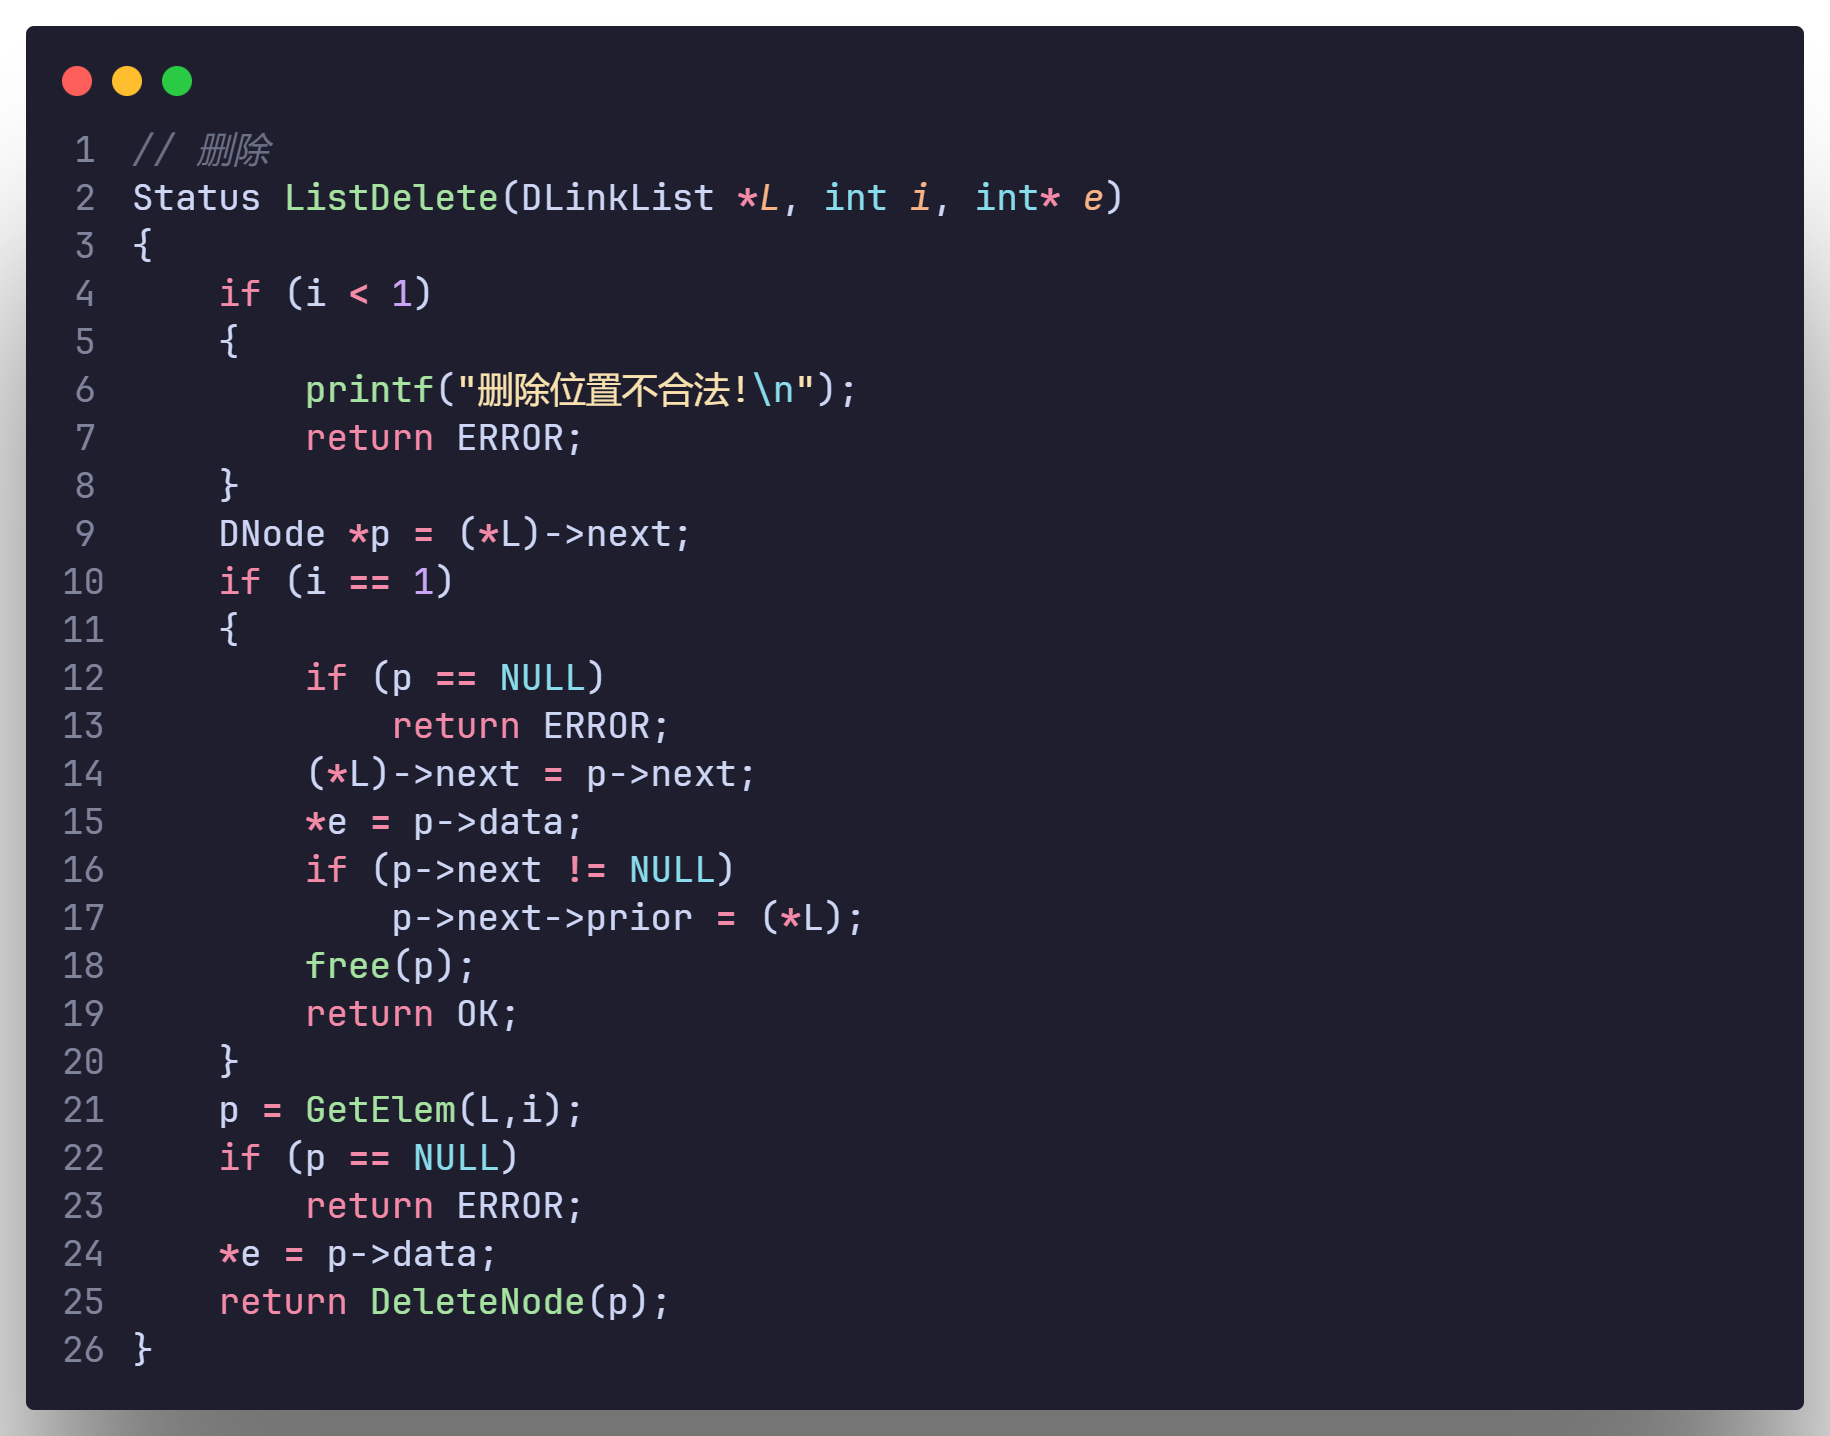
\includegraphics[scale=0.2]{"figure/Note/LinearList/DlDel.png"}
\end{figure}

\subsubsection{双链表辅助函数}

(1). $Length$

\begin{figure}[H]
    \centering
    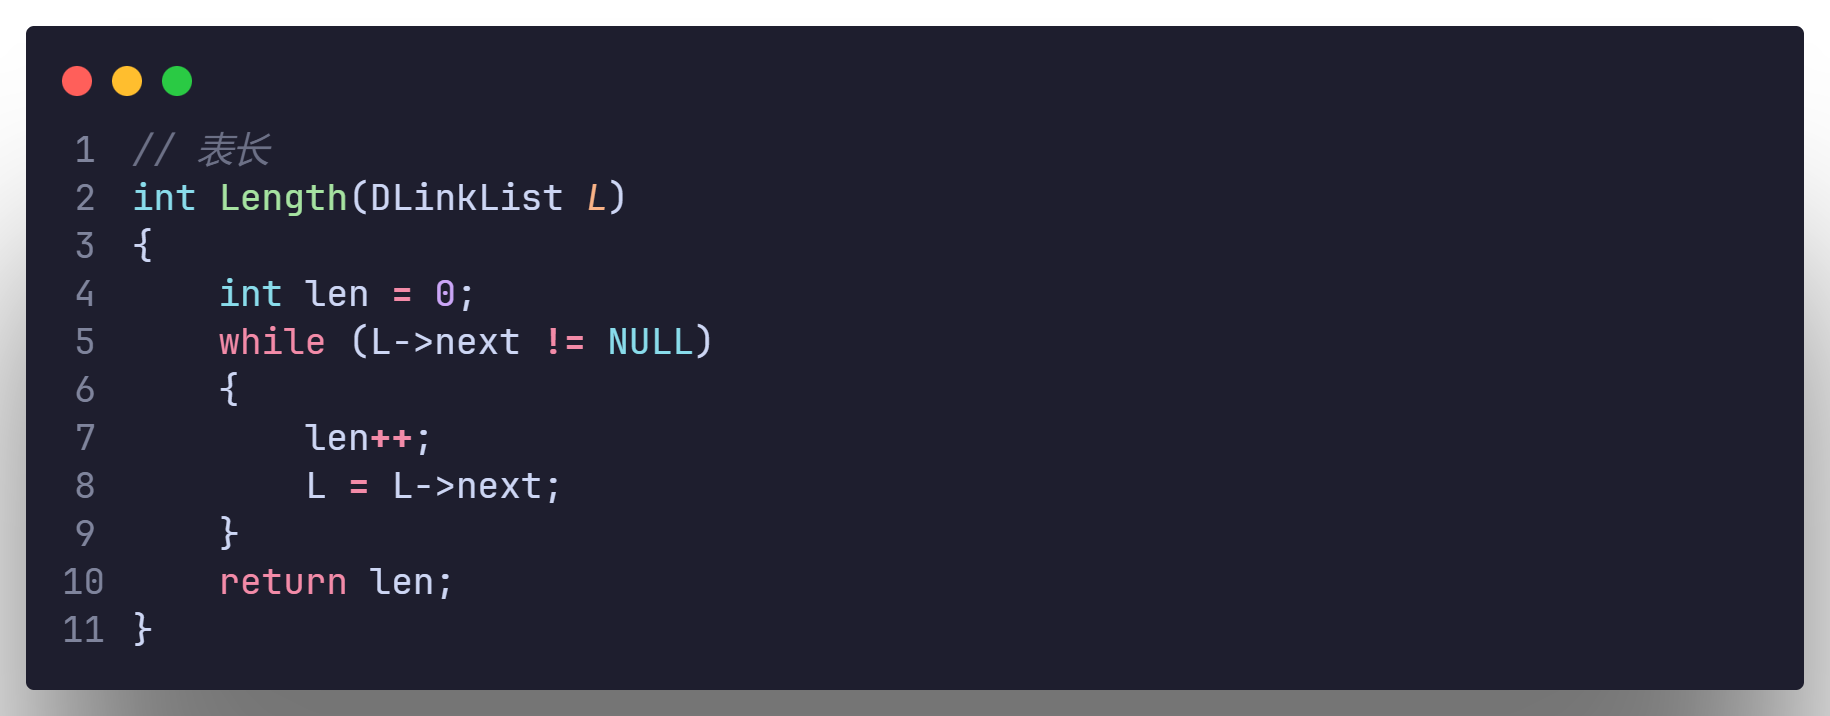
\includegraphics[scale=0.2]{"figure/Note/LinearList/DlLen.png"}
\end{figure}

(2). $Empty$

\begin{figure}[H]
    \centering
    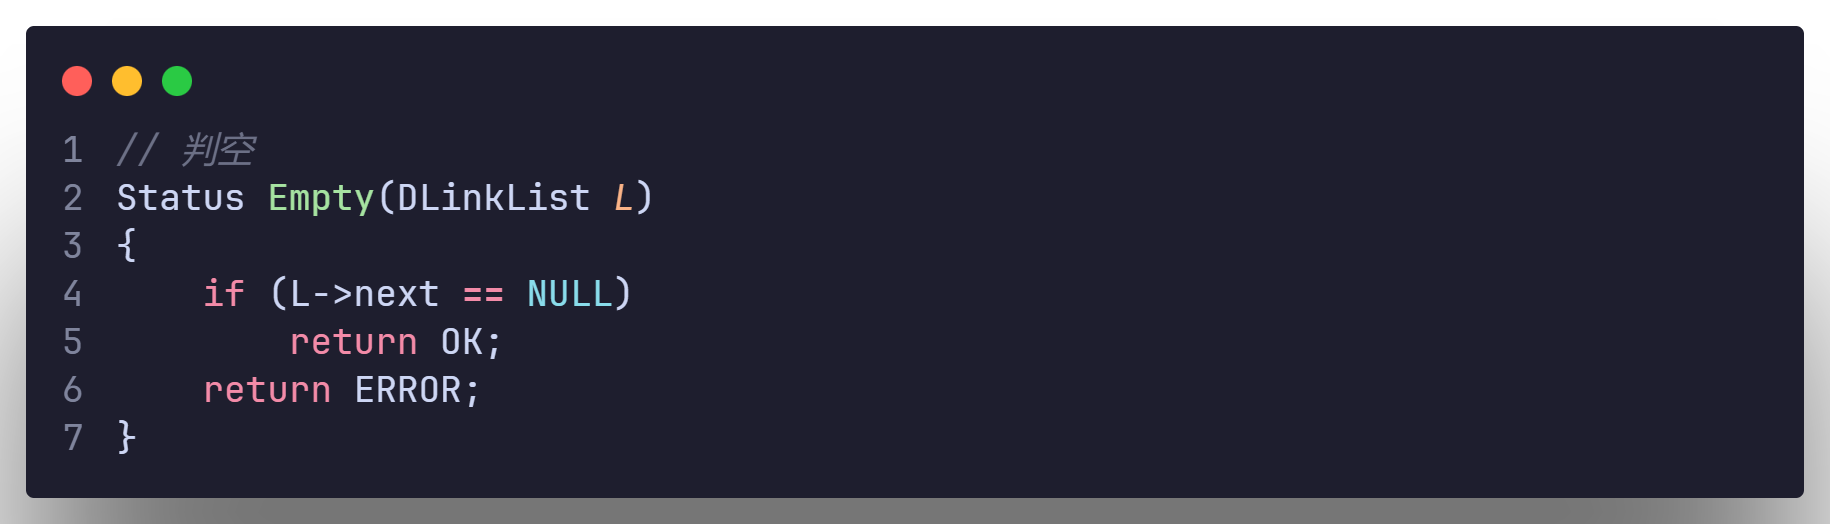
\includegraphics[scale=0.2]{"figure/Note/LinearList/DlEmpty.png"}
\end{figure}

(3). $PrintList$

\begin{figure}[H]
    \centering
    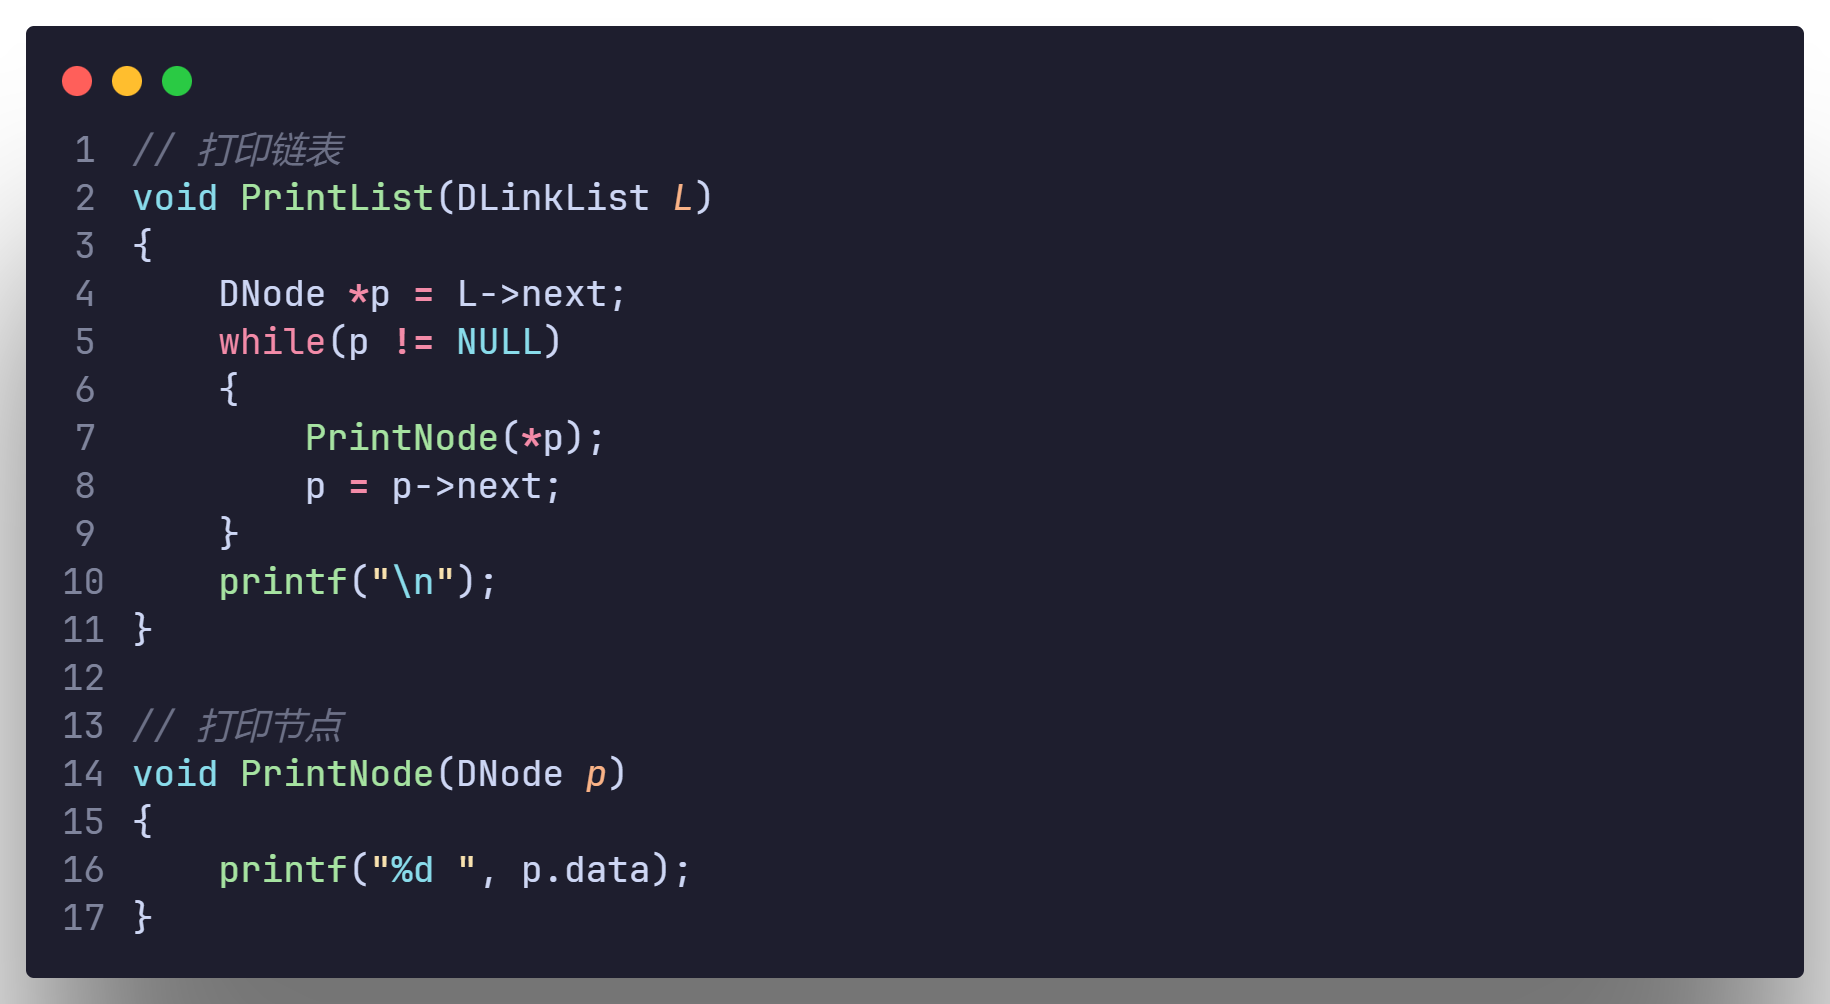
\includegraphics[scale=0.2]{"figure/Note/LinearList/DlPrint.png"}
\end{figure}

\subsubsection{头插法 \& 尾插法}

(1). 头插法

\begin{figure}[H]
    \centering
    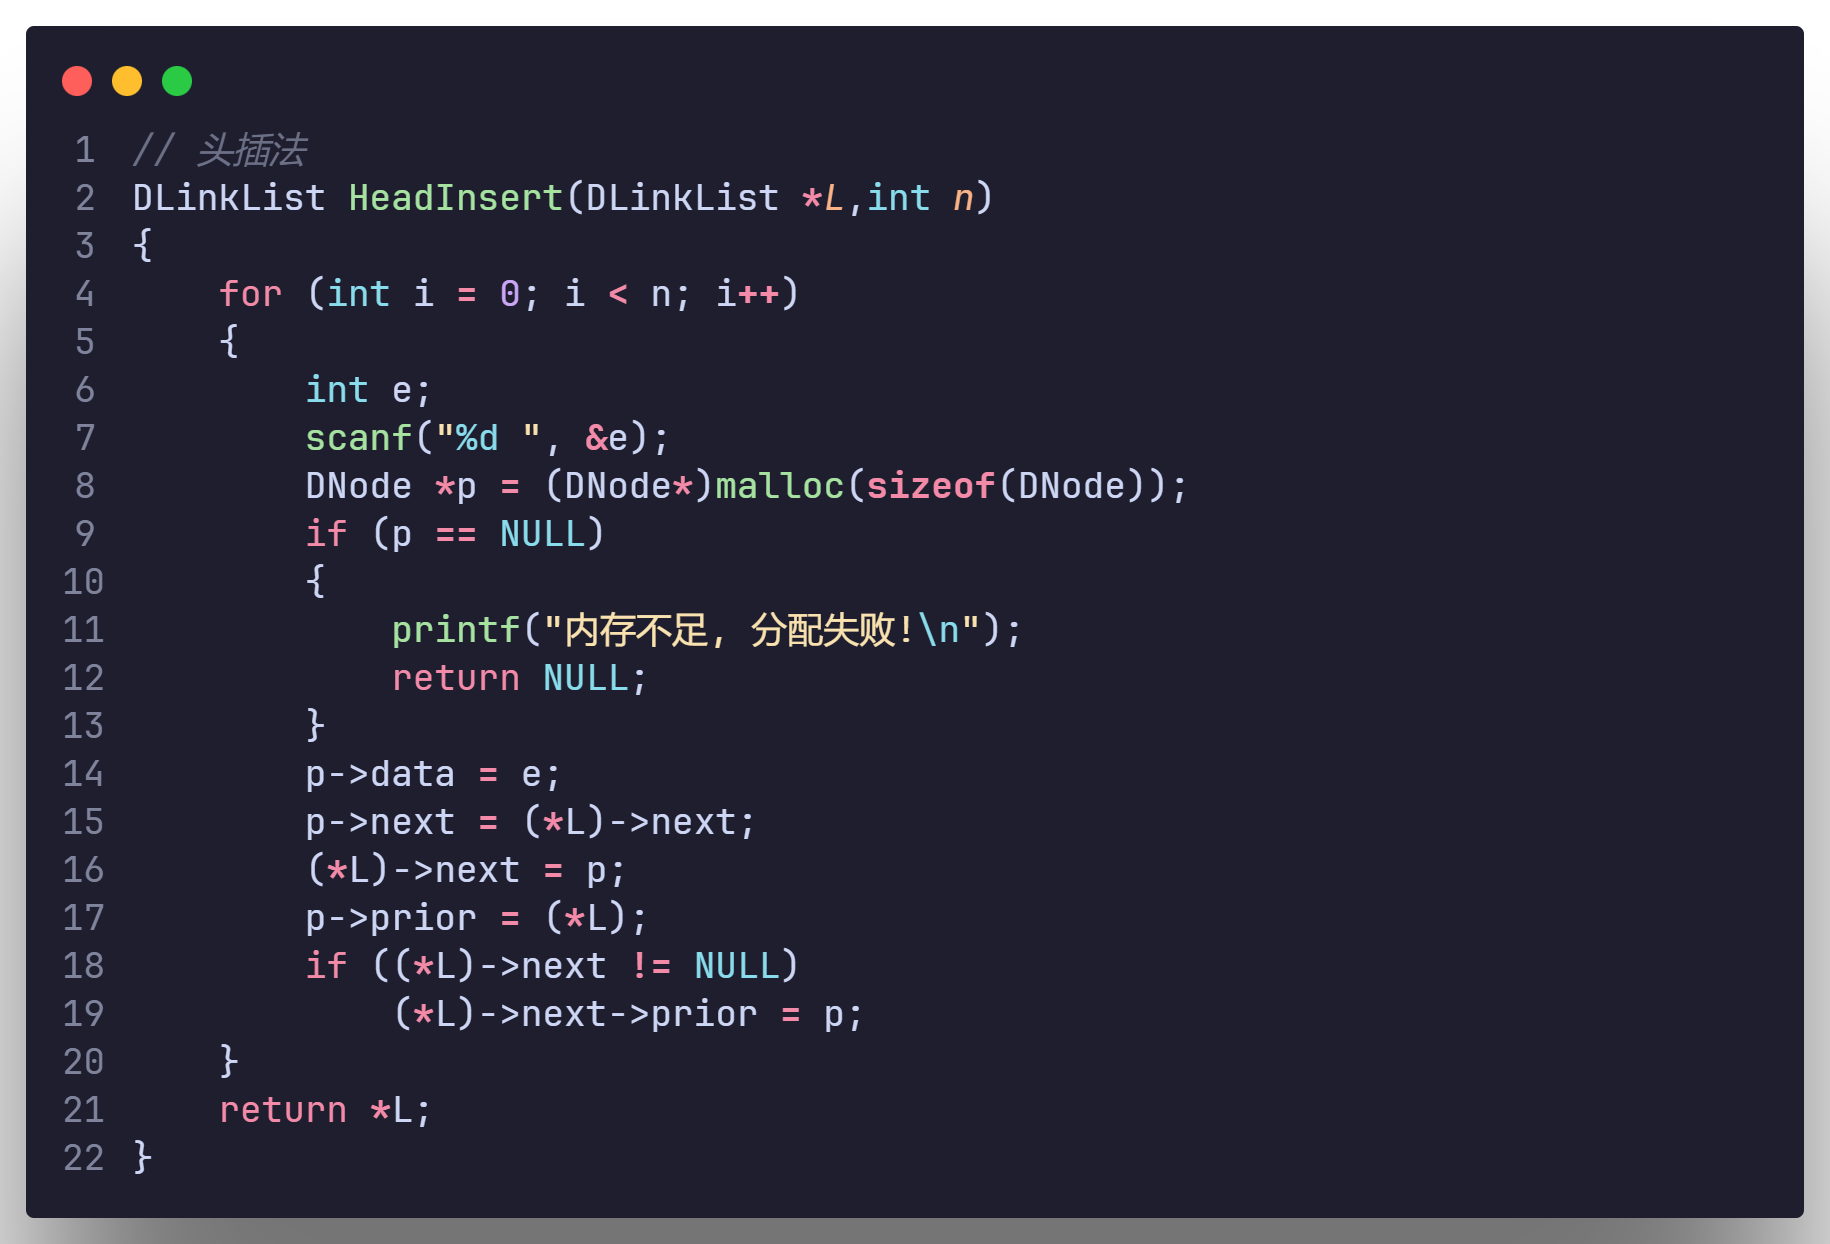
\includegraphics[scale=0.2]{"figure/Note/LinearList/DlHInsert.png"}
\end{figure}

(2). 尾插法

\begin{figure}[H]
    \centering
    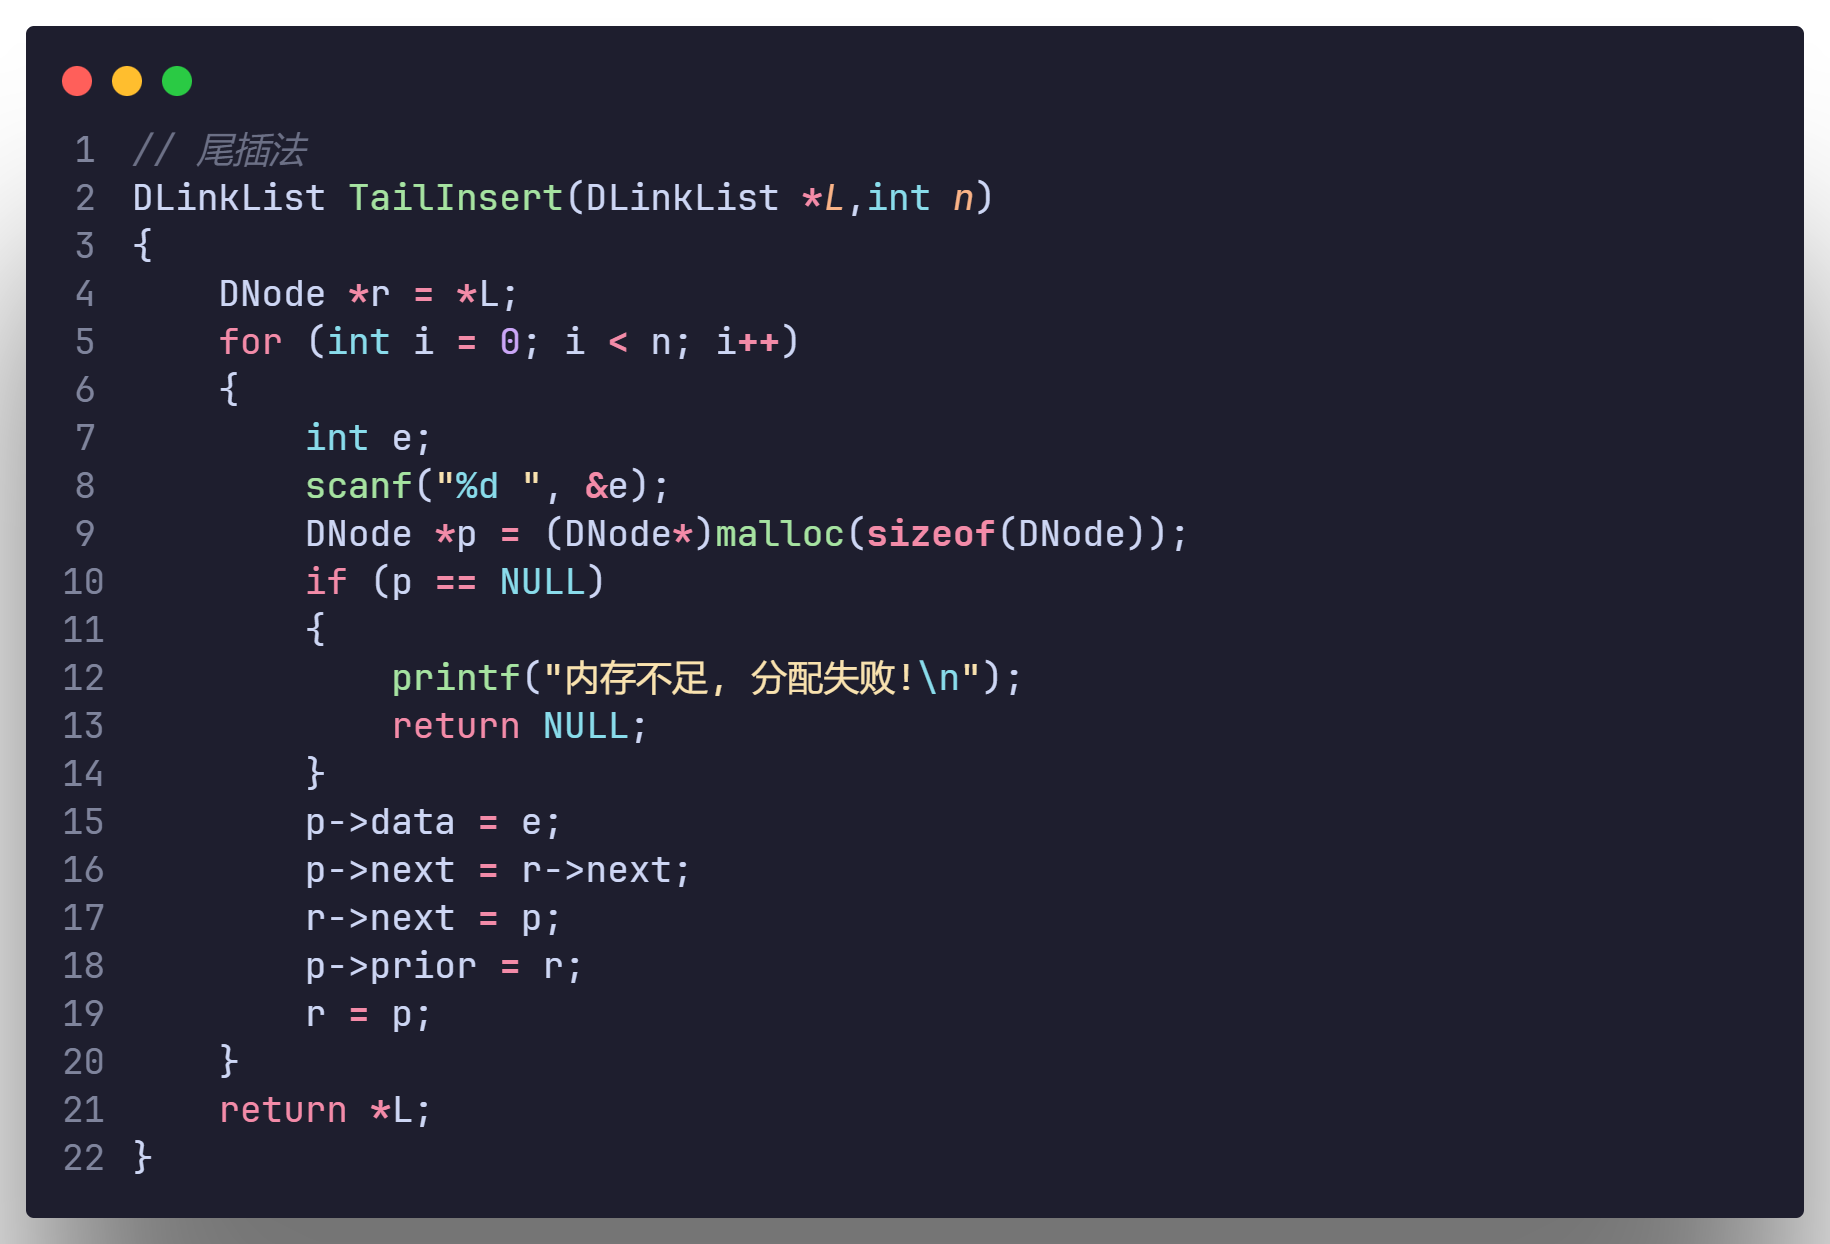
\includegraphics[scale=0.2]{"figure/Note/LinearList/DlTInsert.png"}
\end{figure}

\subsubsection{双链表反转}

\begin{figure}[H]
    \centering
    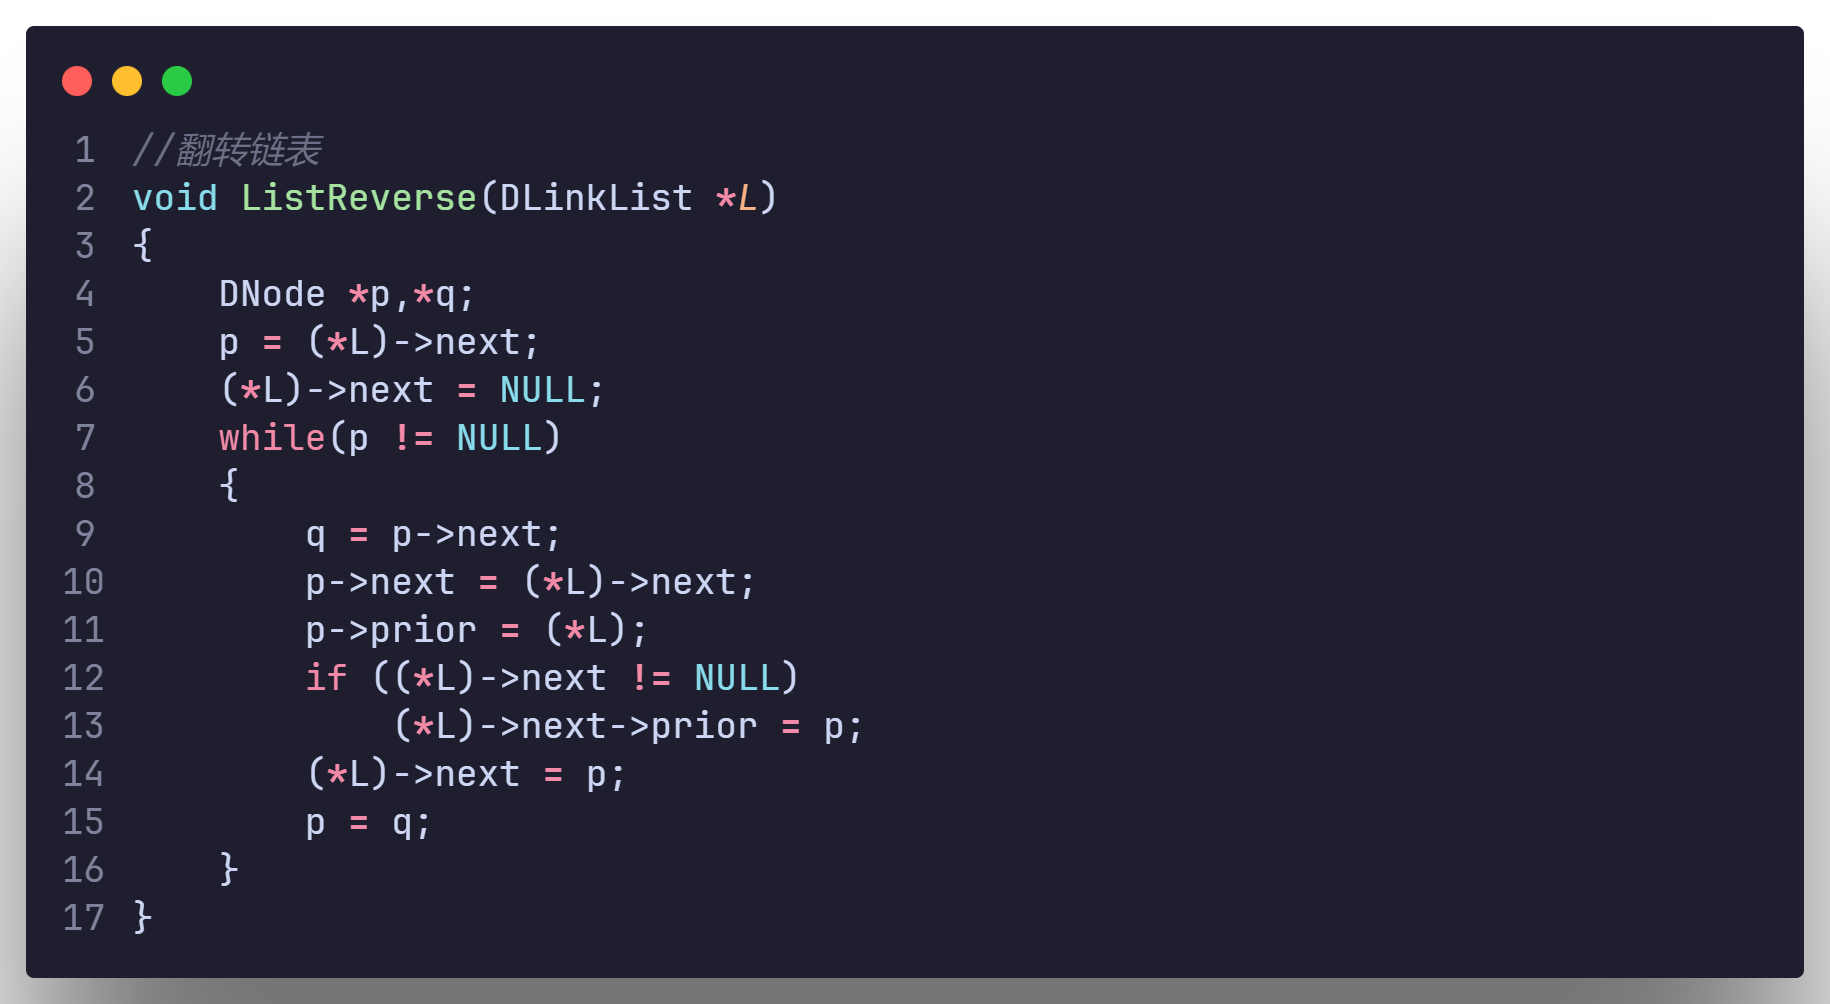
\includegraphics[scale=0.2]{"figure/Note/LinearList/DlReverse.png"}
\end{figure}


\subsection{循环链表}
\begin{definition}[循环链表]
    \begin{enumerate}
        \item 分为循环单链表和循环双链表, 与单链表和双链表的区别在于尾节点指向头节点
        \item 判空操作与单链表、双链表存在差异
        \item 插入、删除、以及判断表头、表尾节点有一定变化
    \end{enumerate}
\end{definition}

\subsection{静态链表}
\begin{definition}[静态链表]
    \begin{enumerate}
        \item 使用数组的链表, 数组第一个元素当做头节点, 每个位置除了保存数据元素外, 还保存下一个元素的位置
        \item 初始化时将所有位置的下一个元素位置清空
        \item 插入、删除操作需要找到上一个节点的位置, 然后将下一个元素位置清空
    \end{enumerate}
\end{definition}
\section{Summary}
\subsection{顺序表与链表比较}
\begin{table}[H]
    \centering
    \caption{顺序表与链表比较}
    \label{table: 顺序表与链表比较}
    \begin{tblr}{
        width = 0.8\textwidth,
        hlines = {1pt},
        hline{1,Z} = {2pt},
        vline{2-Y} = {1pt},
        cell{1}{1} = {r=1,c=2}{c},
        cell{1}{3} = {r=1,c=2}{c,teal7},
        cell{2}{1} = {r=2,c=1}{c},
        cell{2}{2} = {c},
        cell{2}{3} = {r=1,c=2}{l},
        cell{3}{2} = {c},
        cell{3}{3} = {r=1,c=2}{l},
        cell{4}{1} = {r=2,c=1}{c},
        cell{4}{2} = {c},
        cell{4}{3} = {r=1,c=2}{l},
        cell{5}{2} = {c},
        cell{5}{3} = {r=1,c=2}{l},
        cell{6}{1} = {r=2,c=2}{c},
        cell{6}{3} = {r=2,c=2}{l},
    }
    \diagbox{比较项目}{存储结构} &           & 顺序表                                                                  & \\
    空间                       & 存储空间   & {① 预先分配\\  ② 会导致空间闲置或溢出}                                      & \\
                              & 存储密度   & {① $\text{存储密度}=1$\\  ② 不需要额外空间来表示节点的逻辑关系}                & \\
    时间                       & 存取元素   &  {① 随机存取\\ ② 按位置访问元素时间复杂度 $O(1)$}                            & \\
                              & 插入、删除  &  平均移动一半的元素, 时间复杂度 $O(n)$                                      & \\
    适用情况                   &            & {① 表长变化不大,确定变化范围\\ ② 很少进行插入或删除, 经常按照元素位置序号访问数据} & \\
                              &           &                                                                         &\\
    \end{tblr}
    \myspace{1}
    \begin{tblr}{
        width = 0.8\textwidth,
        hlines = {1pt},
        hline{1,Z} = {2pt},
        vline{2-Y} = {1pt},
        cell{1}{1} = {r=1,c=2}{c},
        cell{1}{3} = {r=1,c=2}{c,blue7},
        cell{2}{1} = {r=2,c=1}{c},
        cell{2}{2} = {c},
        cell{2}{3} = {r=1,c=2}{l},
        cell{3}{2} = {c},
        cell{3}{3} = {r=1,c=2}{l},
        cell{4}{1} = {r=2,c=1}{c},
        cell{4}{2} = {c},
        cell{4}{3} = {r=1,c=2}{l},
        cell{5}{2} = {c},
        cell{5}{3} = {r=1,c=2}{l},
        cell{6}{1} = {r=2,c=2}{c},
        cell{6}{3} = {r=2,c=2}{l},
    }
    \diagbox{比较项目}{存储结构} &           & 链表                                                            & \\
    空间                       & 存储空间   & {① 动态分配 \\  ② 不会出现空间闲置或溢出}                            & \\
                              & 存储密度   & {① $\text{存储密度}<1$\\ ② 需要借助指针来表示节点的逻辑关系}          &\\
    时间                       & 存取元素   & {① 顺序存取\\ ② 按位置访问元素时间复杂度 $O(n)$}                     &\\
                              & 插入、删除  & 不需要移动元素, 确定插入或删除位置后,时间复杂度 $O(n)$                 &\\
    适用情况                   &            &{① 表长变化很大\\ ② 频繁进行插入或删除操作}                            &\\
                              &           &                                                                 &\\
    \end{tblr}
\end{table}

\subsection{单链表、双链表、循环链表比较}
\begin{table}[H]
    \centering
    \caption{单链表、双链表、循环链表比较}
    \label{table: 单链表、双链表、循环链表比较}
    \small
    \begin{tblr}[m]{
        width = \textwidth,
        colsep = {0.5pt},
        hlines = {1pt},
        hline{1,Z} = {2pt},
        vline{2-Y} = {1pt},
        cells = {c},
    }
    \diagbox{链表名称}{操作名称}       & {查找\\表头节点}                                & {查找\\表尾节点}                                           & {查找节点 $\mathbf{*p}$\\ 前驱节点} \\
    {带头节点\\单链表 $L$}             & {$\mathbf{L->next}$\\ 时间复杂度 $O(1)$}   & {从 $\mathbf{L->next}$ 依次向后遍历\\ 时间复杂度 $O(n)$} & 无法找到前驱节点\\
    {带头节点头指针 $L$\\ 循环单链表}   &  {$\mathbf{L->next}$\\ 时间复杂度 $O(1)$}   & {从 $\mathbf{L->next}$ 依次向后遍历\\ 时间复杂度 $O(n)$} & {$\mathbf{p->next}$可以找到前驱节点\\ 时间复杂度 $O(n)$}\\
    {带头节点尾指针 $R$\\ 循环单链表}   & {$\mathbf{R->next}$\\ 时间复杂度 $O(1)$}    &  {$\mathbf{R}$\\ 时间复杂度 $O(1)$}                    & {$\mathbf{p->next}$可以找到前驱节点\\ 时间复杂度 $O(n)$}\\
    {带头节点\\双向循环链表 $L$}       & {$\mathbf{L->next}$\\ 时间复杂度 $O(1)$}    &  {$\mathbf{L->prior}$\\ 时间复杂度 $O(1)$}             & {$\mathbf{p->prior}$可以找到前驱节点\\ 时间复杂度 $O(1)$} \\
    \end{tblr}
\end{table}
